\documentclass[11pt, a4paper]{article}
%
%
% PACKAGES ---------------------------------------------------------------
%
\usepackage[utf8]{inputenc}
\usepackage[T1]{fontenc}
\usepackage{amsmath}
\usepackage{amsfonts}
\usepackage{amssymb}
\usepackage{enumitem}
\usepackage[normalem]{ulem}
\usepackage[mathscr]{euscript}
%\usepackage{calrsfs}
\usepackage{dsfont}
\usepackage{float}
\usepackage{times}
\usepackage{bbm}
\usepackage{xcolor}
\usepackage{xparse}
\usepackage[left=2.5cm, right=4.5cm, bottom=3cm, top=3cm,marginparwidth=4cm]{geometry}
\usepackage{comment}
\usepackage{cprotect}

\usepackage{microtype}
\usepackage{mhequ}

\usepackage{xstring}


\usepackage{tcolorbox}
\usepackage{tikz}
\usepackage{tikz-cd} 

\usepackage[colorlinks,linkcolor=blue,citecolor=blue,urlcolor=blue]{hyperref}
\usepackage{amsthm}

\usepackage[capitalise]{cleveref}







\newtheorem{theorem}{Theorem}[section]
\newtheorem{lemma}[theorem]{Lemma}
\newtheorem{proposition}[theorem]{Proposition}
\newtheorem{corollary}[theorem]{Corollary}

\theoremstyle{definition}
\newtheorem{definition}[theorem]{Definition}
\newtheorem{assumption}[theorem]{Assumption}
\newtheorem{condition}[theorem]{Condition}
\newtheorem{exercise}[theorem]{Exercise}


\theoremstyle{remark}
\newtheorem{remark}[theorem]{Remark}
\newtheorem{example}[theorem]{Example}

\numberwithin{equation}{section}














\newcommand{\eqdef}{\stackrel{\mbox{\tiny\rm def}}{=}}
\newcommand{\eqlaw}{\stackrel{\mbox{\tiny\rm law}}{=}}



%\usepackage{comment}

\usetikzlibrary{calc}
\usetikzlibrary{arrows}

\renewcommand{\ttdefault}{lmtt}

\def\dash{\leavevmode\unskip\kern0.18em--\penalty\exhyphenpenalty\kern0.18em}
\def\slash{\leavevmode\unskip\kern0.15em/\penalty\exhyphenpenalty\kern0.15em}

\colorlet{darkblue}{blue!90!black}
\colorlet{darkred}{red!80!black}
\colorlet{darkgreen}{green!50!black}
\let\comm\comment
\def\martin#1{\comm[darkblue]{MH: #1}}
\def\luca#1{\comm[darkred]{LG: #1}}
\def\xuemei#1{\comm[darkgreen]{XML: #1}}

\long\def\martinText#1{{\color{darkblue}Martin:\ #1}}


% THEOREM Environments ---------------------------------------------------
%

\crefname{example}{Example}{Examples}
\Crefname{example}{Example}{Examples}

\crefname{assumption}{Assumption}{Assumptions}
\Crefname{assumption}{Assumption}{Assumptions}

\crefname{condition}{Condition}{Conditions}
\Crefname{condition}{Condition}{Conditions}

% COMMANDS ---------------------------------------------------------------
%
\renewcommand{\labelenumi}{(\roman{enumi})}
\renewcommand{\theenumi}{\labelenumi}
\renewcommand{\labelitemi}{$\triangleright$}
\setlist{topsep=1ex, itemsep=0.5ex, before={\setlist{topsep=-.5ex}}}

\DeclareMathOperator{\diag}{diag}
\DeclareMathOperator{\ran}{ran}
\DeclareMathOperator{\rank}{rank}
\DeclareMathOperator{\spann}{span}
\DeclareMathOperator{\supp}{supp}
\DeclareMathOperator{\diam}{diam}
\DeclareMathOperator{\trace}{tr}
\DeclareMathOperator{\var}{var}
\DeclareMathOperator{\ent}{Ent}
\DeclareMathOperator{\sign}{sign}
\DeclareMathOperator{\cv}{conv}
\DeclareMathOperator{\Div}{div}


\newcommand{\A}{\ensuremath{\mathcal{A}}}
\newcommand{\B}{\ensuremath{\mathcal{B}}}
\newcommand{\C}{\ensuremath{\mathcal{C}}}
\newcommand{\D}{\ensuremath{\mathcal{D}}}
\newcommand{\cE}{\ensuremath{\mathcal{E}}}
\newcommand{\cN}{\ensuremath{\mathcal{N}}}
\renewcommand{\S}{\ensuremath{\mathscr{S}}}
\newcommand{\Sloc}{\ensuremath{\mathscr{S}_{\mathrm{loc}}}}
\newcommand{\Q}{\ensuremath{\mathscr{Q}}}
\newcommand{\Qloc}{\ensuremath{\mathscr{Q}_{\mathrm{loc}}}}
\newcommand{\F}{\ensuremath{\mathcal{F}}}
\newcommand{\G}{\ensuremath{\mathcal{G}}}
\renewcommand{\H}{\ensuremath{\mathscr{H}}}
\newcommand{\h}{\ensuremath{\mathfrak{h}}}
\newcommand{\K}{\ensuremath{\mathbb{K}}}
\renewcommand{\L}{\ensuremath{\mathcal{L}}}
\newcommand{\M}{\ensuremath{\mathcal{M}}}
\newcommand{\N}{\ensuremath{\mathbb{N}}}
\renewcommand{\P}{\ensuremath{\mathcal{P}}}
\newcommand{\R}{\ensuremath{\mathbb{R}}}
\newcommand{\X}{\ensuremath{\mathcal{X}}}
\newcommand{\1}{\ensuremath{\mathbf{1}}
}\newcommand{\Y}{\ensuremath{\mathcal{Y}}}
\newcommand{\Z}{\ensuremath{\mathcal{Z}}}
\newcommand{\sY}{\ensuremath{\mathscr{Y}}}
\newcommand{\W}{\ensuremath{\mathcal{W}}}
\newcommand{\cW}{\ensuremath{\mathscr{W}}}
\def\law{{\mathrm {law}}}
\def\id{{\mathrm {id}}}

\def\ff#1#2{\textstyle{\frac{#1}{#2}}}
\let\f\frac
\def\epsilon{\varepsilon}
\def\le{\leq}
\NewDocumentCommand{\Lip}{om}{\IfNoValueTF{#1}{|#2|_{\mathrm{Lip}}}{|#2|_{\mathrm{Lip};\,#1}}}
\def\range{{\mathrm {Range}}}
\newcommand{\define}{\ensuremath\triangleq}
\newcommand{\expec}[1]{\mathbb{E}[#1]}
\def\E{\mathbb E}
\def\X{\mathcal X}
\newcommand{\Expec}[1]{\mathbb{E}\left[#1\right]}
\newcommand{\norm}[1]{\ensuremath\left\|#1\right\|}
\newcommand{\hilb}{\ensuremath{\mathcal{H}}}
\newcommand{\tr}[1]{\ensuremath\trace[#1]}
\newcommand{\Tr}[1]{\ensuremath\trace\left(#1\right)}
\newcommand{\braket}[1]{\ensuremath\langle#1\rangle}
\newcommand{\Braket}[1]{\ensuremath\left\langle#1\right\rangle}
\newcommand{\prob}{\ensuremath\mathbb{P}}
\newcommand{\tv}[1]{\ensuremath{\|#1\|_{\mathrm{TV}}}}
\newcommand{\TV}[1]{\ensuremath{\left\|#1\right\|_\mathrm{TV}}}
\renewcommand{\Re}{\mathrm{Re}}
\renewcommand{\Im}{\mathrm{Im}}
\renewcommand{\geq}{\geqslant}
\renewcommand{\leq}{\leqslant}
\def\CC{{\mathcal C}}
\def\BC{{\mathrm BC}}
\def\${|\!|\!|}
\def\B{{\mathcal B}}
\def\F{{\mathcal F}}
\def\<{\langle}
\def\>{\rangle}
\def\dom{\mathrm{Dom}}
\def\cov{\mathrm {cov}}
\newcommand{\vertiii}[1]{{\left\vert\kern-0.25ex\left\vert\kern-0.25ex\left\vert #1 \right\vert\kern-0.25ex\right\vert\kern-0.25ex\right\vert}}
\newcommand{\rom}[1]{(\textup{\uppercase\expandafter{\romannumeral#1}})}
\def\sgn{{\mathop {\rm sign}}}
\newcommand{\tdelta}{\delta'}

%\definecolor{DarkGreen}{HTML}{6B38FF}
%%\definecolor{DarkGreen}{rgb}{0.0, 0.6, 0.0}
\definecolor{LB}{rgb}{0.29, 0.63, 0.73}

%\newcommand{\xml}[1]{\textcolor{LB}{#1---xuemei}}
%\newcommand{\martin}[1]{{\leavevmode\color{red!70!black}#1---martin}}
%\newcommand{\luca}[1]{{\leavevmode\color{blue}#1---luca}}


%%%%%% Luca added
\newcommand{\scal}{\mathcal{S}} %scaling/translation operator
\newcommand{\Cc}{\mathcal{C}_c} %Denote smooth compactly supporte
\newcommand{\Ccinf}{\mathcal{C}_c^\infty} %Denote smooth compactly supporte
\newcommand{\cH}{\mathcal{H}}% Hilbert space for Malliavin
\newcommand{\bD}{\mathbb{D}} % Malliavin space
\newcommand{\cU}{\mathcal{U}} % EW solution
\newcommand{\nueff}{\nu_{\mathrm{eff}}} %effective variance
\renewcommand{\deg}{\textnormal{deg}} %deg label
\newcommand{\tfrk}{\mathfrak{t}} %label map t(.)
\newcommand{\bbullet}{\textcolor{blue}{\bullet}} % blue vertices
\newcommand{\obullet}{\textcolor{orange}{\bullet}} % orange vertices
\newcommand{\tx}{\tilde{x}}

\renewcommand*{\thefootnote}{(\arabic{footnote})} %% footnote with parenthe

\let\eps\varepsilon
\let\d\partial

\makeatletter

\DeclareRobustCommand{\TitleEquation}[2]{\texorpdfstring{\StrLeft{\f@series}{1}[\@firstchar]$\if%
b\@firstchar\boldsymbol{#1}\else#1\fi$}{#2}}

\makeatother



%\DeclareMathOperator{\cov}{cov}

\date{Version: \today}
%\footnote{\protect\version}\newcommand{\version}{\spaceskip=0pt \normalshape Version as of \today.}

\begin{document}
\title{
	Fluctuations of stochastic PDEs with long-range correlations
}
\author{Luca Gerolla\footnote{Imperial College London, \texttt{luca.gerolla16@imperial.ac.uk}}, 
    Martin Hairer\footnote{EPFL \& Imperial College London, \texttt{martin.hairer@epfl.ch}},  and Xue-Mei Li\footnote{EPFL \& Imperial College London, \texttt{xue-mei.li@epfl.ch}}}

\maketitle
\begin{abstract}
We study the large scale fluctuations of the solution of a nonlinear stochastic heat equation (SHE) in dimensions $d \geq 3$ driven by a multiplicative Gaussian noise, white in time and coloured in space with non-integrable spatial covariance  decaying at the rate of $|x|^{-\kappa}$, with $\kappa \in (2, d)$.  Motivated by recent works on SHE and KPZ driven by noise with compactly supported spatial correlation, we show that the fluctuations converge to the solution of a stochastic heat equation with an explicit additive spatially correlated noise that has a Riesz kernel of degree $-\kappa$ as its spatial covariance. The convergence of the fluctuations is shown  to take place in the optimal Hölder topologies.   
\end{abstract}
\vspace{2em}

{
{\it Mathematics Subject Classification: } 60H15, 60H05, 60F05


{\it Keywords:} stochastic heat equation, fluctuations, large scale dynamics, non-integrable\\ \indent spatial correlation
}


%{\hypersetup{hidelinks}
\tableofcontents
%}
\pagestyle{plain}

\section{Introduction}
We study the long term statistical properties of  solutions to the non-linear stochastic heat equation (SHE) on $\R^d$ with a multiplicative random forcing: 
\begin{equ}
\label{eq:basic_mSHE}
\partial_t u(t,x)=\ff 12 \Delta u (t,x)+\beta \sigma(u(t,x)) \xi(t,x), \qquad u_0 \equiv 1\;,
\end{equ}
where $\sigma$ is a real valued function on $\R$ and $\xi$ is a mean zero Gaussian noise that is white in time and coloured in space, with non-integrable correlation. This interesting equation enjoys popularity coming from its connection, through the Cole--Hopf transform \cite{Bertini-Giacomin-97}, with the KPZ (Kardar--Parisi--Zhang) equation, directed polymers,
and the exclusion process model.  

Formally, if $u$ solves \eqref{eq:basic_mSHE} with $\sigma(u) =u$, then $h = \log u$ solves the KPZ equation
\begin{equ}\label{eq:basic_KPZ}
\partial_t h = \tfrac{1}{2} \Delta h +
\tfrac{1}{2} |\nabla h |^2 
+ \beta \xi, \quad \quad h(0, x) = 0.
\end{equ}
Introduced by \cite{kardar1986dynamic} as a model of surface growth,  the KPZ equation has been used widely since then to capture universal behaviour of many important physics and probabilistic models.  
The Cole--Hopf transform is  rather formal: when $\xi$ is a space-time white noise, 
the nonlinear equation \eqref{eq:basic_KPZ} is ill-posed while in contrast the stochastic heat equation with space-time white noise makes perfect sense as an Itô equation.

A rigorous and stable notion of solution to the KPZ equation in $d=1$ can be obtained by using
the theory of controlled rough paths \cite{hairer_solvingKPZ}, the general
framework of regularity structures \cite{hairer_RegStr}, or the paracontrolled calculus approach of \cite{gubinelli2015paracontrolled, gubinelli2017kpz}.  
These theories, see also \cite{kupiainen2016renormalization, Duch} for a third
approach closer in spirit to Wilson's renormalisation group, revolutionised the 
field of (\emph{subcritical}) singular SPDEs. But none of these theories apply in higher dimensions, 
as these equations in higher dimensions typically become \emph{supercritical}.


In fact, the rescaled soluton
$\epsilon^{\frac 12} h({\epsilon^{-\frac 32}}t,  \epsilon^{-1}   x )$ to the KPZ equation in dimension one converges, as $\epsilon \to 0$, up to shifting and scaling, to a universal space-time process, now known as the KPZ fixed point.  This was a long standing conjecture proven only recently in \cite{quastel2020convergence, virag2020heat}, but 
built on steady progress over the past couple of decades (cf.\ 
\cite{baik1999distribution, amir_corwin_quastel_2011probability, Balazs-Quastel-Seppalainen2011,alberts_khanin_quastel2014intermediate, matetski_quastel_remenik2016-21kpz}, see also the surveys \cite{quastel2011introduction,corwin2012kardar,quastel_spohn2015one} and more recently \cite{corwin2019some, remenik2022integrable, baik2022kpz}). 
The KPZ fixed point is a universal non-Gaussian limit process, by now relatively well understood, to which a large class of growth models (referred to as the KPZ class) is expected to converge (at large scales) after suitable scaling. Zooming in, i.e.\ considering $\epsilon^{-\frac 12} h(\epsilon^2t,  \epsilon x )$, the scaling limit of the KPZ equation is the solution to the stochastic heat equation driven by
additive space-time white noise, sometimes also called the Edwards--Wilkinson (EW) model. 
Growth models with large scale scaling limit given by that process are said to belong to the Edwards--Wilkinson class. The KPZ equation interpolates between the (Gaussian) EW model (at small scales) and the non-Gaussian KPZ fixed point (at large scales) \cite{corwin2012kardar, quastel2011introduction}. 




In the present article, we are interested in the stochastic heat equation with coloured noise in the high-dimensional case $d \geq 3$.
It has recently been shown in a number of works \cite{gu18edwards, magnen2018scaling, dunlap2020_KPZ_fluctuations, cosco2020law, lygkonis2020edwards, gu20_nlmSHE,gu_komorowski21_kpz_torus_fluct,dunlap2018homo, comets2018fluctuation} that, provided that the correlations of the 
driving noise have compact support (or at least decay sufficiently fast), both the SHE and KPZ equation exhibit Gaussian fluctuations at 
large scales in 
the weak disorder phase, namely when $\beta$ is sufficiently small.
The limiting fluctuations are described by the Edwards--Wilkinson model. 
%The limiting fluctuations are described by the Edwards--Wilkinson model with the variance of the additive space time noise given by $\int_{\R^d} R(x) \E [Z(x)Z(0)] dx$, where $Z$ is a stationary field
%describing the behaviour of solutions at large times.
In this article, we are interested in the case of \textit{non-integrable} decay of correlations for
the driving noise. We show that in this case 
one still obtains a Gaussian fluctuation theorem, but the limiting process exhibits spatial correlation 
with power law decay. 


\subsection{Main Results}

We let $u$ be as in \eqref{eq:basic_mSHE} and, for $\eps > 0$, we write $u_\eps(t,x) = u(t/\eps^2, x/\eps)$. 
Given a test function $g$,  we furthermore set
\begin{equ} 
X_t^{\epsilon, g}=\epsilon^{1-\frac \kappa 2}\int_{\R^d}  \bigl( u_\epsilon(t,x)-\E u_\epsilon(t,x)\bigr)g(x) dx.
\end{equ}
Note that  here $\E u_\epsilon(t,x) = 1$ by our assumption on the initial condition, and it is  straightforward to see that the law of large numbers holds.

We assume throughout that the Gaussian noise $\xi$ satisfies $\E \xi(t,x)\xi(s,y) = \delta(t-s) R(x-y)$
with a covariance $R$ satisfying the following.
\begin{assumption}\label{assump-cov}
	The covariance $R: \R^d\to \R$ is smooth, positive definite, and there exists $ c_R >0$ with
	\begin{equ}\label{eq:R_decay_bounded}
	| R(x)| \leq \frac{c_R}{1 + |x|^\kappa} \quad \text{with} \quad \kappa \in (2, d)\;.
	\end{equ}
	Furthermore, for any $x \in \R^d \setminus \{0\}$,
	\begin{equ}\label{ass:R_conv}
	\epsilon^{-\kappa} R( \epsilon^{-1}x ) \to |x|^{-\kappa} \quad \text{as} \quad \epsilon \to 0.
	\end{equ}
	Finally, for any $\delta \in (0,1)$, the Fourier transform $\hat{R}$ of $R$ satisfies 
	\begin{equ}\label{eq:R_transf_int}
	\int_{\R^d} \frac {\hat{R}(z)} {|z|^{2\delta}} dz < \infty.   
	\end{equ}
\end{assumption}

\begin{example}
	The function $R(x) = (1+  |x|^2)^{-\kappa/2}$ satisfies the 
	above assumption. %\luca{CHECK} 
\end{example}



\begin{theorem} \label{thm:basic-convergence}  
	Let $d\geq 3$, let $\sigma$ be Lipschitz continuous, 
	and let $\xi$ be a mean zero space time Gaussian noise with $\E [ \, \xi_t(x) \xi_s(y)\,]=\delta(t-s) R(x-y)$ where $R$ satisfies Assumption~\ref{assump-cov} (so in particular it has power law decay with exponent $\kappa \in (2,d)$).
	Then, there exists a $\beta_0>0$ such that for all $\beta < \beta_0$, and for any time indices 
	$0 < t_1 \leq \dots \leq t_n$, and for any
	smooth functions with compact support $\{g_i\}_{i =1, \dots, n}~\subset~\Ccinf(\R^d)$,  the following random variables converge, as $\epsilon\to 0$, in distribution: 	$$  (X_{t_1}^{\epsilon,g_1}, \dots, X_{t_n}^{\epsilon,g_n}) \Rightarrow \bigg(\int_{\R^{d}} \cU(t_1,x) g_1(x) \, dx, \dots , \int_{\R^{d}} \cU(t_n,x)  g_n(x) \, dx\bigg). $$
where $\cU$ is  the solution of the stochastic heat equation with additive correlated Gaussian noise:
\begin{equ}[e:limitEW]
	\partial_t \cU(t,x)=\ff 12 \Delta \cU (t,x) + \beta \nueff \, \dot W^\kappa (t,x), \qquad \cU(0, \cdot) \equiv 0.
\end{equ}
where  $\nueff^2 = \lim_{t \to \infty} |\E [ \sigma (u(t,0))]|^2$ is the effective variance and the covariance of the Gaussian noise is
	\begin{equ} \label{eq:EW_noise_covariance_defn}
	\E [\,\dot W^\kappa(t,x) \dot W^\kappa(s,y)\,]= \delta(t-s) |x-y|^{-\kappa}.
	\end{equ}
\end{theorem}

\begin{remark}
 At present  it is unclear what would happen with $\kappa \leq 2$ and in the edge case $\kappa =d$.
In the latter case one would expect to see Gaussian fluctuations, but with a logarithmic correction in the scaling, similarly to what happens in dimension $2$. In the case $\kappa < 2$ on the other hand, one
expects to see a situation similar to the case of white noise in dimension $1$ with some
non-trivial scaling exponents. 
\end{remark}

In Section~\ref{sec:weak_convergence}, we also show that $X^\epsilon$ converges weakly to $\cU$ as a  H\"{o}lder continuous distribution-valued stochastic process. 
\begin{theorem}\label{thm:weak_conv_1}
Given the assumptions of Theorem~\ref{thm:basic-convergence},
for any $\alpha < -1 \wedge (1-\frac \kappa 2) $ and any positive $\gamma < \frac 1 2  - \frac 1 2(\frac \kappa 2 + \alpha)_+$,	there exists $\beta_{\gamma,\alpha} >0$ such that, for any $\beta <\beta_{\gamma,\alpha}$, $X^\epsilon$ converges to $\cU$ weakly in $\C^\gamma ([0,T], \C^{\alpha})$, for any $T >0$.
\end{theorem}


\begin{remark}
For $\alpha$ sufficiently negative we can take $\gamma$ close to $\frac 12$.
The dependence of the upper bound on $\beta$ on $\alpha, \gamma$ is only technical, it is used to control the high moments of $u$. 
	Note also that $u_\epsilon$  solves the equation
	\begin{equ}\label{eq:rescaled_eqn_kappa}
	\partial_t u_\epsilon(t,x)=\ff 12 \Delta u_\epsilon(t,x)+\beta \epsilon^{\frac \kappa 2 -1}  \sigma(u_\epsilon(t,x)) \xi^\epsilon(t, x), \qquad u_\epsilon(0, x) \equiv 1\;,
	\end{equ}
	where $\xi^\epsilon (t,x)$ is a white in time Gaussian noise with spatial covariance $\epsilon^{-\kappa} R(\frac{x}{\epsilon})$ and the product is interpreted in the Itô integral sense. 	
	From assumption \eqref{ass:R_conv}, it is immediate that $\xi^\epsilon$ converges in law to a spatially correlated noise with covariance $|x|^{-\kappa}$.  By a simple reasoning the law of large numbers $u_\eps \to \E u_\eps = 1$ holds, but this is in fact
	validated a posteriori by Theorem~\ref{thm:weak_conv_1}.  Since $v_\eps = \epsilon ^{1-\kappa/2} ( u^\epsilon -1) $ solves \eqref{eq:rescaled_eqn_kappa} but without the factor $\eps^{\frac \kappa 2 -1}$ and since $u_\eps \to 1$, one would naïvely expect that in the limit \eqref{e:limitEW} one 
	has $\nueff = \sigma(1)$, but this is in fact incorrect due to resonances between the fluctuations of
	$u_\eps$ and $\xi^\eps$.

We now give a heuristic argument leading to the correct expression 
$\nueff^2 = \lim_{t \to \infty} |\E [ \sigma (u(t,0))]|^2$.
For this, we test the rescaled noise term in \eqref{eq:rescaled_eqn_kappa} against a test function $g$, thus considering the expression
$$\int_{\R^d}  \int_0^t  \sigma(u_\epsilon(s,x))g(x)\; \xi^\epsilon(ds,dx),$$
whose covariance is given by 

\begin{equ}[e:covarSimple]
\int_{\R^{2d}}  \int_0^t C(\eps^{-2}s, \eps^{-1}(x-y)) \,ds\, \epsilon^{-\kappa} R(\ff {x-y} \epsilon) g(x) g(y)\, dx\,dy\;,
\end{equ}
where we set
\begin{equ}
C(s,x) = \E [ \sigma(u(s,0)) \sigma(u(s,x))]\;.
\end{equ}
As in \cite{MSZ16_weak_strong_mshe}, we expect $u$ to converge in law to some stationary process $Z$ as $t\to \infty$, we expect $C(s,\cdot)$ to
 converge as $s\to \infty$ to some bounded function $\bar C: \R^d\to \R$ which, assuming that $Z$ is sufficiently mixing so the spatial correlation vanishes, furthermore has the asymptotics
$\lim_{|x| \to \infty} \bar C(x) = |\E \sigma(Z)|^2 = \nueff^2$.



In case $R$ is integrable so is $R \bar C$ and we expect \eqref{e:covarSimple}
to converge (provided $\kappa = d$) to $\tilde \nu^2 \|g\|_{L^2}^2 t$ with
$$\tilde \nu^2 = \int_{\R^d}\bar C(y) R(y)\, dy\;,$$
thus leading to the limit equation $\d_t \cU=\ff 12 \Delta  \cU +\beta \tilde \nu  \xi$ where $\xi$ 
is standard space time white noise.
For $R$ with compact support, this heuristic agrees with the result  in \cite{MSZ16_weak_strong_mshe,gu18edwards}, see also \cite{cosco2020law}. 
 
In our case $R$ is not integrable,  $\tilde \nu^2 =\infty$ for the SHE, but we have instead the large scale structure $\epsilon^{-\kappa} R(\frac{x-y}{\epsilon}) \approx |x-y|^{-\kappa}$. Since this is integrable near $0$, we expect \eqref{e:covarSimple} to behave like 
\begin{equ}
t \int_{\R^{2d}}  \bar C(\eps^{-1}(x-y)) \frac{ g(x) g(y)}{|x-y|^{\kappa}}\, dx\,dy
\approx t \nueff^2 \int_{\R^{2d}}  \frac{ g(x) g(y)}{|x-y|^{\kappa}}\, dx\,dy\;,
\end{equ}
which is precisely what is suggested by Theorem~\ref{thm:weak_conv_1}.
\end{remark}


\begin{remark}
	The isotropic convergence assumption \eqref{ass:R_conv} can be relaxed to 
	\begin{equation*}
	\epsilon^{-\kappa} R( \epsilon^{-1}x ) \to \theta\big(\tfrac x {|x|}\big) |x|^{-\kappa} \quad \text{as} \quad \epsilon \to 0,
	\end{equation*}
	for some non-negative bounded function $\theta: \partial B(0,1) \to \R_+$. This results in an Edwards--Wilkinson limit driven by Gaussian white noise with covariance
	\begin{equation*}
	\E [\, \dot W^\kappa(t,x) \dot W^\kappa(s,y)\,]= \delta(t-s) \,\theta\big(\tfrac {x-y} {|x-y|}\big) |x-y|^{-\kappa},
	\end{equation*}
	in place of \eqref{eq:EW_noise_covariance_defn}.	
\end{remark}


%\subsection{Discussion}


\begin{remark}
In space dimension $2$, the KPZ equation driven by space-time white noise is scaling critical 
and its behaviour is still not completely understood,
except in a ``weak coupling'' regime (and its boundary case \cite{KPZ2D1}) where it 
exhibits Gaussian fluctuations
\cite{CSZ17-universality,caravenna2019moments_CSZ18a,gu2020gaussian_KPZ_2D,CSZ20-KPZ-full-subcritical,tao2022gaussian}. In fact, the \textit{anisotropic} KPZ equation (where the nonlinearity is
given by $(\d_x h)^2-(\d_y h)^2$)
is now somewhat better understood
thanks to the fact that it (formally) admits the free field as its invariant distribution.
In that case, one again observes Gaussian fluctuations, but with an interesting $\sqrt{|\log \epsilon|}$ 
correction to the diffusive scaling \cite{AKPZ2D1,AKPZ2D2,MR4499841,AKPZ2D3}.
\end{remark}




\subsection{Proof and organisation of the paper}

 To prove the main result we first establish preliminary estimates:  uniform moment bounds for $u(t,x)$, convergence rates for $u(t,0)$, we then apply Stein's method as in \cite{huang18-2020Stein_CLT_mshe}, see Proposition~\ref{prop:multi_Stein}, so it is sufficient to show that the quantity  
$\langle DX^{\epsilon, g}_t, v^{\epsilon,g}_t \rangle_{\cH} - \Sigma^{g}_t$ 
converges to zero in $L^2(\Omega)$, where $\Sigma^{g}_t$ is the covariance of the 
solution $\cU$ to the stochastic heat equation. 
We will decompose this difference into the (deterministic) difference of covariances $\Delta \cov$  between $X^\epsilon$ and $\cU$, which can be easily seen to converge to zero by direct computation, and a 
remainder term $\Delta_\epsilon$.


The main technical hurdle is to  control the $L^2(\Omega)$ norm of this residual term $\Delta_\epsilon$,
which is achieved by bounding it by a multiple integral involving singular kernels. These integrals
are bounded by recasting them as Feynman diagrams. In Lemma~\ref{lem:diagram_integration} below, we 
adapt to our needs the general framework of \cite{hairer2016analyst_BPHZ}, allowing us to show 
that $\Delta_\epsilon \to 0$ as $\epsilon\to 0$. The restriction to small values $\beta<\beta_0$ is used 
when deriving uniform bounds on the solution $u$ and its Malliavin derivative; we refer to the beginning of Section~\ref{sec:proof-thm1} for more details.

The proof of Theorem~\ref{thm:weak_conv_1} follows by tightness of $X^\epsilon$ in $\C^\gamma ([0,T], \C^\alpha)$ for suitable $\gamma<\frac 1 2$ and $\alpha <-1$. This is shown by formulating a Kolmogorov type criterion (Proposition~\ref{prop:time-holder_distribution_process-app}) and leveraging uniform moment bounds. We review the spaces $\C^\alpha\subset \S^\prime$ in the beginning of Section~\ref{sec:weak_convergence}.


\medskip\noindent\emph{Organisation}. In Section~\ref{sec:prelims} we collect some basic Gaussian\slash covariance estimates, the key Feynman diagrams integration Lemma~\ref{lem:diagram_integration}, moment bounds, and decorrelation estimates on $u$. Section~\ref{sec:proof-thm1} is devoted to the proof of Theorem~\ref{thm:basic-convergence}, whereas the proof of tightness and Theorem~\ref{thm:weak_conv_1} are in Section~\ref{sec:weak_convergence}. 


\subsubsection*{Acknowledgements}

This research was supported by the Royal Society through MH's research professorship,  by the 
EPSRC through XML's  grant EP/V026100/1, and by the CDT grant EP/S023925/1 where the latter is 
co-investigator. LG is supported by the EPSRC Centre for Doctoral Training in Mathematics of 
Random Systems: Analysis, Modelling 
and Simulation (EP/S023925/1).



\subsubsection*{Notation and conventions}
$\bullet$ We assume $(\Omega, \F, \mathbb{P})$ is a complete probability space supporting the Gaussian noise $\xi$ and we denote by $\| \cdot \|_p$ the $L^p(\Omega)$ norm.\\
$\bullet$ We write $\hat f(z) = \int_{\R^d} f(x) e^{-i z \cdot x}dx$ for the Fourier transform of $f$. \\
$\bullet$ Whenever $a\lesssim b$, we mean $a \leq C b$ for some constant $C>0$ independent of $\epsilon$.\\
$\bullet$ Throughout the following sections (see Lemma \ref{lem:moments} and onwards) the coupling threshold $\beta_0$ and implicit inequalities constants $C$ will depend on $d, R$ and $\sigma$, we avoid keeping track of this to lighten notation.\\
$\bullet$ We denote with $\sigma_{Lip}$ the Lipschitz constant of the nonlinearity $\sigma$.\\
$\bullet$  For $E\subset \R^d$ open, we write $\Ccinf(E)$ for the set of  smooth functions on $E$ with compact support, and we set $\D = \Ccinf(\R^d)$.\\
$\bullet$ For $r \in [0,1)$,
we denote by $\C^{r} = \C^{r}(\R^d, \R)$ the space of little-Hölder continuous functions, which is
separable and Fréchet with system of seminorms
\begin{equ}
\| f \|_{E, \C^r}  := \sup_{
	\substack{x, y \in E \\x\neq y }
} \frac{|f(x) - f(y)|}{|x-y|^ r}\;,
\end{equ}
where $E \subset \R^d$ is open.
For $r \ge 1$, the space $\C^r$ is defined recursively as the space of continuously differentiable functions such that each directional derivative is in $\C^{r-1}$. We denote by $\C^r_c = \C^r \cap \Cc$ the subset of H\"{o}lder continuous compactly supported functions.

\section{Preliminary estimates}\label{sec:prelims}
The product term on the right-hand side of the multiplicative stochastic heat equation \eqref{eq:basic_mSHE}
 is interpreted as an It\^o integral. Given the flat initial condition $u(0,x) \equiv 1$, the mild solution of the equation is given by the solution to the fixed point problem
\begin{equ} \label{eq:mild_soln}
u(t,x) = 1 + \beta \int_{0}^{t} \int_{ \R^d} P_{t-s}(x-y) \sigma(u(s,y)) \xi(ds, dy), 
\end{equ}
where $P_{t}(x) = (2\pi t)^{-d/2} e^{-\frac{|x|^2}{2t}}$ denotes the $d$-dimensional heat kernel. The theory on the well-posedness of  mild solution
is classic \cite{walsh1986introduction, daPrato_Inf}.
In fact assuming $\sigma$ is Lipschitz continuous  and
since $R$ is bounded below in our setting, according to
 	 \cite[Thm~0.2]{peszat2000nonlinear} (based on \cite{peszat1997stochastic}), the necessary and sufficient conditions for $u$ to be function valued is that  the spectral measure $\hat{R}$ satisfies ``Dalang's condition'':
\begin{equ}\label{eq:dalangs_plain_condition}
\int_{\R^d} \frac{\hat{R}(z)}{1+|z|^2} dz <\infty,
\end{equ}
which in our case follows from assumption \eqref{eq:R_transf_int}. The existence and uniqueness results in \cite[Thm~13, Remark~14]{dalang1999extending} was proved in the martingale measures framework of \cite{walsh1986introduction}.

 

\subsection{Elementary Gaussian and covariance estimates}

In this subsection we gather the main estimates involving the Gaussian kernel and covariance $R$ used below. Firstly, we have the following pointwise estimates. 

\begin{lemma}\label{lem:gaussian_time_bounds}
	Given any $\lambda \in (0,  d)$, the following bounds hold uniformly in $\tau \geq s >0$, and  $x \in \R^d\setminus\{0\}$:
	\begin{equs}
	P_{\tau}(x)  &\lesssim s^{-
	 \frac \lambda 2} |x|^{\lambda - d}, \label{eq:comp_est} \\
	|\nabla_x P_{\tau}(x)|  &\lesssim  s^{-1-\frac \lambda 2} |x|^{1+\lambda - d}.             \label{eq:comp_est_grad}
	\end{equs}
\end{lemma}
\begin{proof}
It suffices to recall that $|D_x^k P_t(x)| \lesssim (\sqrt{|t|} + |x|)^{-d-|k|}$.
\end{proof}

Given $\kappa \in (2, d)$, the kernel $| \cdot|^{-\kappa}$ is integrable near $0$ and has sufficient decay at infinity so that the following estimates hold.
\begin{lemma} \label{lem:gaussian_cov_est}
	Assume that $|R(x)| \leq \frac{c_R}{1 + |x|^\kappa}$, where   $\kappa \in (2, d)$. Then
	for any $r > 0$, any $x \in \R^d$, any $\lambda < \kappa$ and $\delta \geq0$, 	
	\begin{equs}
		\int_{\R^{2d}} P_r(z_1) P_r(z_2) \big| R(z_1 -z_2)\big| dz_1 dz_2 &\lesssim 1 \wedge r^{-\f \kappa 2},\quad \label{eq:control_time} \\
		\int_{\R^{2d}} P_r(z_1-x) P_r(z_2)\big| R(z_1 -z_2)\big| dz_1 dz_2 dr
		& \lesssim 1 \wedge \big( r^{-\frac \lambda 2} (1 \wedge |x|^{\lambda - \kappa}) \big),\qquad  \label{eq:time_decay_est}\\
		\int_0^\infty \int_{\R^{2d}} P_{r+\delta}(z_1-x) P_r(z_2) \big|R(z_1 -z_2)\big| dz_1 dz_2 dr
		& \lesssim 1 \wedge |x|^{2-\kappa}.
		\label{eq:control_space}
	\end{equs} 
\end{lemma}
\begin{proof}
Firstly, through a change of variable and convolution of Gaussian kernels,
\begin{equs}
	&\int_{\R^{2d}} P_{r+\delta}(z_1-x) P_r(z_2) \big|R(z_1 -z_2)\big| dz_1 dz_2 \\&\qquad =   \int_{\R^d} P_{2r+\delta} (z-x) \big|R(z)\big|dz 
	\leq c_R \Big( 1 \wedge \int_{\R^d}\frac{ P_{2r+\delta} (z-x) } {|z|^{\kappa}} dz\Big).
\end{equs}
Then, with $\delta =0$, $x=0$ and given $\kappa <d$,  we obtain \eqref{eq:control_time} bounding the following:
\begin{equ}
	\int_{\R^d}\frac{ P_{r} (z) } {|z|^{\kappa}} dz = r^{- \f \kappa 2} \int  
	\frac{ P_1(z)} {|z|^{\kappa}} dz \lesssim r^{-\kappa/2}. 
\end{equ}
Whereas, using the pointwise estimate \eqref{eq:comp_est} and $|R(x)| \leq \frac{c_R}{1 + |x|^\kappa}$, we derive 
\eqref{eq:time_decay_est},
\begin{equ}
	\int_{\R^d} P_{2r} (z-x) \big|R(z)\big| dz  
	\leq {c_R} \Big( 1 \wedge (2r)^{-\frac \lambda 2 }
	\int_{ \R^d} \frac{|z-x|^{\lambda -d}}{1 + |z|^\kappa} dz \Big) \lesssim 1 \wedge \big( r^{-\frac \lambda 2} (1 \wedge |x|^{\lambda - \kappa}) \big).
\end{equ}

For \eqref{eq:control_space}, we 
integrate $P_{2r}(x -z)$ over time, obtaining 
\begin{equ}
	\int_0^\infty \int_{\R^d} P_{2r+\delta} (z-x) \big|R(z)\big|dz \leq 
	\int_0^\infty \int_{\R^{d}} P_{2r}(z-x)  \big|R(z)\big| dz dr  = c_d \int_{\R^d} \frac {|R(z)|} {|z-x|^{d-2}} dz. 
\end{equ}
Since $\kappa \in (2,d)$, the proof for estimate \eqref{eq:control_space}
is complete with Lemma~\ref{lem:controlR} below.
\end{proof}


\begin{lemma}\label{lem:controlR}
Assume that $|R(x)| \leq \frac{c_R}{1 + |x|^\kappa}$, where   $\kappa \in (2, d)$. Then,
\begin{equ}\label{eq:control_R}
\int_{\R^d} \frac {|R(z)|} {|z-x|^{d-2}} dz   \lesssim 1 \wedge |x|^{2-\kappa}.
\end{equ}
\end{lemma}
\begin{proof}
See for example \cite[Lem.~10.14]{hairer_RegStr}.
\end{proof}

In the case of $R$ bounded and $L^1$-integrable (e.g.\ $\kappa >d$ or compactly supported $R$) the estimates \eqref{eq:control_time}-\eqref{eq:control_space} hold with $\kappa$ replaced by $d$. In the following subsection we introduce a framework to handle systematically integration of multiple kernels and their associated small \slash large scale behaviours. 


\subsection{Feynman diagrams and integration lemma}
\newcommand{\cV}{\mathcal{V}}
The aim of this section is to formulate a criterion (Lemma~\ref{lem:diagram_integration}) to verify that integrals $I_\Gamma$ of the form \eqref{eq:I_Gamma} are finite. We now introduce the notions needed from the general framework of \cite{hairer2016analyst_BPHZ}.  

In our setting, a Feynman diagram $(\cV_*, \cE_*)$ is a finite directed graph, with $\cV_*$ the collection of vertices and $\cE_*$ is the collection of edges $\cE_* = \{ (e_-, e_+) : e \in \cE_* \}$. We 
further assume that the vertices are partitioned as $\cV_* = \cV_\ell \sqcup \cV_i$, and we refer to 
elements of $\cV_\ell$ as ``legged vertices''\footnote{In the general setting of \cite{hairer2016analyst_BPHZ}, these are precisely the vertices that are target of some incoming leg (at most one in our specific case).}.
Each vertex will represent an integrating variable and, given $x \in (\R^d)^{\cV_*}$ and $A \subset \cV_*$,
we will denote by $x_A \in (\R^d)^{A}$ the restriction of $x$ to $A$.

%% Labels, deg and Kernel behaviour
We also assume that we are given a label map $e \mapsto \tfrk(e) \in \L_*$, where $\L_*$ is a 
finite set of labels, as well as ``degree'' maps $\deg_0 \colon \L_* \to \R_-$ and $\deg_\infty \colon \L_* \to \R_-$. 
To each label $\tfrk$ we associate a kernel $K_\tfrk$ (smooth except possibly at the origin), with small \slash large scale behaviour captured by $\deg_0 \tfrk $ and $\deg_\infty \tfrk$ respectively. More precisely, we assume that
\begin{equ} \label{eq:deg_ineq}
| K_\tfrk (x)|  \leq c_1  |x|^{\deg_0  \tfrk} \, \1_{|x|\leq 1}, \qquad 
| K_\tfrk (x)|  \leq c_2  |x|^{\deg_\infty  \tfrk} \, \1_{|x| > 1}. 
\end{equ}
In the next section we indicate edge labels by colour \slash degree in the diagram and we 
omit orientation of the edges since all kernels will be symmetric. 

%% Integral - diagram relation
Given such a diagram $\Gamma $, we associate to $\Gamma$ a distribution $I_\Gamma$ on $(\R^d)^{\cV_\ell}$
by
\begin{equ} \label{eq:I_Gamma}
I_\Gamma(\phi) := \int_{(\R^{d})^{\cV_*}} \prod_{e \in \cE_*} K_{\tfrk(e)} (x_{e_+} - x_{e_-}) \, \varphi(x_{\cV_\ell})\, dx,
\end{equ}
Our test functions will typically be of the form $\varphi(x_{\cV_\ell}) = \prod_{i\in \cV_\ell} g_i(x_i)$ for some $ g_i \in \Ccinf(\R^d)$.

In general, the integral \eqref{eq:I_Gamma} may diverge and the main point of this section is to 
introduce a criterion which guarantees that this is not the case.
For this, we now introduce the notions of subgraph and tight partition of $\Gamma$, as defined in \cite{hairer2016analyst_BPHZ}.

%% Subgraph and tight partition
A \emph{subgraph} $\bar{\Gamma} \subset \Gamma$ consists of a subset of internal edges $\bar{\cE} \subset \cE_*$, as well as the subset of internal vertices $\bar{\cV} \subset \cV_*$ containing all the vertices incident to at least one edge in $\bar{\cE}$. (But $\bar{\cE}$ does not need to contain all the edges connecting vertices in $\bar{\cV}$.) We consider Feynman diagrams $(\cV_*, \cE_*)$ with at least one edge and partitions $\P_\Gamma = \{ A_i \}$ of $\cV_*$  with  $|\P_\Gamma| \geq 2$, where $A_i$ are disjoint non-empty subsets of $\cV_*$ such that $ \bigcup_{A_i \in \P_\Gamma} A_i = \cV_*$. Then  $\P_\Gamma$  is said to be a \emph{tight partition} if there exists an element $A_0 $ of $\P_\Gamma$ such that $\cV_\ell \subset A_0$. For a given partition $\P_\Gamma$ we denote with  $\cE(\P_\Gamma)$  the set of ``traversing'' edges $e \in \cE_*$ whose ends $e_+$ and $e_-$ are  in different elements of $\P_\Gamma$, i.e.\ $e_+ \in A_i$ and $e_- \in A_j$ with $i\neq j$. 

Then \cite[Prop.~2.3 \& 4.1]{hairer2016analyst_BPHZ} (but see \cite{weinberg1960} for the
original formulation of this fact, as far as the small-scale behaviour is concerned) 
combined give the following:

\begin{lemma}\label{lem:diagram_integration}
	The integral $I_{\Gamma} $ 
	 is finite for any $\varphi \in \Cc((\R^d)^{\cV_\ell})$, if the following holds:\\
(\emph{Small scales}) For every non-empty subgraph $\bar \Gamma \subseteq \Gamma$,
\begin{equ}\label{eq:small_scales_crit}
\deg_0 \,\bar \Gamma := \sum_{e \in \bar \cE} \deg_0 \tfrk(e) + d ( |\bar \cV| - 1) \,\, > \,\,0. 
\end{equ}
(\emph{Large scales})  For every tight partition $\P_\Gamma$, 
\begin{equ}\label{eq:large_scales_crit}
\deg_\infty \, \P_\Gamma := \sum_{e \in \cE(\P_\Gamma)}  \deg_\infty \tfrk(e) + d ( |\P_\Gamma| - 1) \,\,< \,\, 0.
\end{equ}
\end{lemma}

\begin{remark}\label{remark:tree_diagram}
	If $\Gamma$ is a tree (no undirected cycle), 
to check \eqref{eq:small_scales_crit} is sufficient to verify for all  
$e \in \cE_*$
\begin{equ}\label{eq:small_scales_crit_tree}
\deg_0 \mathfrak t (e) > -d.
\end{equ}
\end{remark}

It is appropriate to state here an example, which will be used in the next section.
\begin{example}\label{lem:diagram0_finite}
For any $f,g \in \Cc(\R^d)$, any $\kappa <d$,  and any $\lambda \in (0, \frac \kappa 2)$, 
 \begin{equ} \label{I-Gamma0}
I_{\Gamma_0}(f,g; \lambda) :=  \int_{\R^{4d}} |y_1 -y_2|^{-\kappa} \, \prod_{i=1}^2 |x_i -y_i|^{\lambda-d}
f(x_1) g(x_2) dy dx<\infty.
\end{equ}
\end{example}

Since $\kappa<d$ and $\lambda>0$, by homogeneity $\int |x_2-y_2|^{\lambda-d}|y_1-y_2|^{-\kappa} dy_2$ is a constant multiple of $|y_1-x_2|^{\lambda-\kappa}$
and $\int \int \prod_{i=1}^2  |x_i-y_i|^{\lambda-d}|y_1-y_2|^{-\kappa} \, dy_1dy_2 =C|x_1-x_2|^{2 \lambda -\kappa}$, and that $I_{\Gamma_0}(f,g; \lambda) $ is finite follows from $\kappa<2 \lambda$.
This simple computation is 
a good place to illustrate notation and to demonstrate how to apply Lemma \ref{lem:diagram_integration}. We draw the  Feynman diagram $\Gamma_0$ associate with the integral and its reduced graph $\Gamma_0'$.
 
\begin{center}
\hspace{-5em}
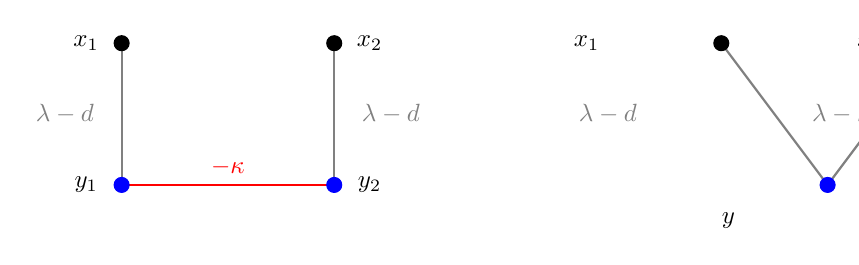
\begin{tikzpicture}[scale=0.9, every node/.style={transform shape}]
%% vertex labels
\node at (-0.5,0) {$y_1$};
\node at (3.5,0) {$y_2$};
\node at (-0.5,2) {$x_1$};
\node at (3.5,2) {$x_2$};
% side vertical edges 
\node at (-0.8, 1) { \textcolor{gray}{$\lambda -d$}};
\node at (3.8 , 1) { \textcolor{gray}{$\lambda -d$}};
%%% edges
\draw[color = red, thick] (0,0) -- (3,0) node [midway, above] {$-\kappa$};
\draw[color = gray, thick] (0,0) -- (0,2);
\draw[color = gray, thick] (3,0) -- (3,2);

%% vertices
\draw[blue, fill=blue] (0,0) circle (3pt);
\draw[blue, fill=blue] (3,0) circle (3pt);
\draw[fill=black] (0,2) circle (3pt);
\draw[fill=black] (3,2) circle (3pt);


\hskip 40pt
\node at (5.0,2) {$x_1$};
\node at (9,2) {$x_2$};
\node at (7,-0.5) {$y$};
% labels
\node at (5.3, 1) { \textcolor{gray}{$\lambda -d$}};
\node at (8.6 , 1) { \textcolor{gray}{$\lambda -\kappa$}};
% edges    +1.4 horizontally 
\draw[color = gray, thick] (6.9,2) -- (8.4,0);
\draw[color = gray, thick] (9.9,2) -- (8.4,0);
% vertices nodes
\draw[black, fill=black] (6.9,2) circle (3pt);
\draw[black, fill=black] (9.9,2) circle (3pt);
\draw[blue, fill=blue] (8.4,0) circle (3pt);
%% no offset
%\draw[color = gray, thick] (5.5,2) -- (7,0);
%\draw[color = gray, thick] (8.5,2) -- (7,0);
%% vertices nodes
%\draw[black, fill=black] (5.5,2) circle (3pt);
%\draw[black, fill=black] (8.5,2) circle (3pt);
%\draw[blue, fill=blue] (7,0) circle (3pt);

\end{tikzpicture}
\\
\hspace{-1.5em}Diagram $\Gamma_0$   
\hskip 116pt Diagram $\Gamma_0'$  \hskip 30pt 
\\ 
\end{center}
The small scales $\deg_0$ and the large scales $\deg_\infty$ of each edge is the same and labelled. To explain the terminology we work with $\Gamma_0$. Note that all 3 labels are greater than $-d$,  the small scale criterion  is trivially satisfied by Remark~\ref{remark:tree_diagram}.
Let $ \cV_\ell = \{ \bullet_{x_1}, \bullet_{x_2}\}$  denote the set of single-legged vertices and the remaining $\cV_i =\{ \bbullet_{y_1}, \bbullet_{y_2} \}$. A tight non-trivial partition must have an element $A_0$ containing $\cV_\ell$, so they are:
 $\P_1= \{ \bullet_{x_1}, \bullet_{x_2},\bbullet_{y_1} \}\cup\{\bbullet_{y_2}\} $, $\P_2= \{ \bullet_{x_1}, \bullet_{x_2},\bbullet_{y_2} \}\cup\{\bbullet_{y_1}\} $,  $\P_3:= \{ \bullet_{x_1}, \bullet_{x_2}\} \cup \{\bbullet_{y_1},\bbullet_{y_2}\} $, and $ \P_4:=\{ \bullet_{x_1}, \bullet_{x_2}\} \cup \{\bbullet_{y_1}\}\cup\{\bbullet_{y_2}\} $. By the Lemma the integral is finite if  $\deg_\infty (\P_i)<0$ for each, which is trivial to check: 
The traversing edges $\P_1$ are: $[y_1, y_2]$ and $[x_2, y_2]$, hence $\deg_\infty (\P_1)=\lambda-d -\kappa+d<0$ in this case, and similarly for $\P_2$, and finally $\deg_\infty \,\P_3  =  2(\lambda-d) + d = 2\lambda -d$, and $\deg_\infty \, \P_4=   2(\lambda-d) -\kappa + 2d = 2\lambda - \kappa <0$. 




\subsection{Moments and large time asymptotics of SHE}
In this subsection,  we  prove some key moment estimates and limit results  for proving Theorem~\ref{thm:basic-convergence} in the next section extending that from \cite{gu20_nlmSHE}. Then, we identify the effective variance $\nueff$ and prove a spatial covariance estimate (Lemma~\ref{lem:Du_L2+cov_estimate}) with the Clark--Ocone formula. 

\noindent \textbf{Notation.} We view $\xi$ as an isonormal Gaussian process on the Hilbert space $\mathcal{H}$,  the closure\footnote{In fact, $R$ is in principle allowed to be 
such that there
are non-trivial elements with zero norm, in which case we also quotient them out.} of $\Ccinf(\R \times \R^d)$ under the inner product 
$$  \langle f , g  \rangle_\cH = \int_{-\infty}^{\infty} \int_{\R^{2d}} f(s, y_1) g(s, y_2) R(y_1-y_2) dy_1 dy_2 ds.
$$
Thus, $\E [  \xi(f) \xi(g)] =  \langle f , g  \rangle_\cH $ for $f, g \in \cH$. 
By  \eqref{eq:control_space} in Lemma~\ref{lem:gaussian_cov_est}, the heat kernel belongs to $\cH$, 
provided  $|R(x)| \leq \frac{c_R}{1 + |x|^\kappa}$ with $\kappa \in (2, d)$.


We consider the space $\bD^{1,2} \subset L^2(\Omega)$ of real valued random variables $X$ 
such that the following norm is finite 
\begin{equ}
\| X \|^2_{\bD^{1,2}} :=  
\E \big( |X|^2 \big)
+ \E \big( \| DX\|_\cH^2  \big), 
\end{equ}
where $D$ is the Malliavin derivative operator. 
We also denote $DX$ by $D_{\cdot,\cdot}X$ for a function valued representative of the Malliavin derivative of $X$  (among its equivalence class in $\cH$). Then $D_{r,z}X$ will denote the pointwise evaluation of $D_{\cdot,\cdot}X$ at $(r , z)$ in $ \R \times \R^d$, which makes sense up to modification on zero Lebesgue measure subsets of $ \R \times \R^d$. For example, if $h \in \cH \cap L^2(\R^{d+1})$ is a deterministic measurable function in $\cH$, then $D_{r,z}  \xi(h) = h(r,z)$. 
We denote by $\delta: \bD^{1,2}(\cH) \to L^2(\Omega)$ the adjoint of $D$, also referred to as divergence or Skorokhod integral.
If $w \in \dom \, \delta$ is $\F_t$-adapted, the Skorokhod integral $\delta(w)$ coincides with the It\^o integral 
$\int_{\R \times \R^d} w(s,y) \xi(ds,dy)$.

By \cite[Prop.~1.3.8]{nualart2006malliavin}, sufficiently regular elements $v \in \dom \,  \delta$ 
satisfy the commutation relation
\begin{equ}\label{eq:commutation_D_adjoint}
D_{r,z} \delta(v) = v(r,z) + \int_{-\infty}^\infty \int_{\R^{d}} D_{r,z} v(s,y) \xi(ds,dy).
\end{equ}
The integral on the right-hand side is in the It\^o sense as long as $D_{r,z} v(s,y)$ is $\F_s$-adapted (in general it is a Skorokhod integral). The equality holds as elements of $\cH$.

Combining the commutation relation \eqref{eq:commutation_D_adjoint} with the mild formulation of the
solution $u$ allows for a useful characterisation of its Malliavin derivative \cite[p.~5]{gu20_nlmSHE} 
and to derive the estimates below, see \eqref{eq:moment_Du}. 
The identity \eqref{eq:commutation_D_adjoint} will also be used in the next section to express the Malliavin derivative of the fluctuations $X^{\epsilon,g}_t$. Given the Lipschitz assumption on $\sigma$, we have $D_{r,z}\sigma(u(s,y)) = \Sigma(s,y) D_{r,z} u(s,y)$ for $\Sigma$ a bounded and adapted process (if $\sigma$ is continuously differentiable then $\Sigma(s,y) = \sigma'(u(s,y))$).

The results in \Cref{lem:moments}  and \Cref{thm:stat_field}
were shown in \cite[Lem.~2.1--2.2, Thm 1.1]{gu20_nlmSHE} for the case when $R$ is compactly supported.
The pointwise bounds on the Malliavin derivative
rely on the following estimate where we allow for non-negative covariance $R$. This is inspired by  \cite[Lemma 2.2]{chen2019comparison},
% and \cite[Thm 6.4]{chen2019spatial}), 
however we are not able to prove the obvious extension to their lemma, in any case the lemma below is sufficient for our use.
 
 Let $\B_+( \R_+ \times \R^d)$ denote the set of measurable functions from $\R_+ \times \R^d$ to $ \R_+$ and a map 
$J_t(s,x): \Pi^2\B_+( \R_+ \times \R^d)\to \R$ as follows
$$J_t(s,x)(g_1, g_2)=\int_{ \R^{2d}} 
		P_{t-s}(x-y_1)P_{t-s}(x-y_2)| R(y_1-y_2)| g_1(s, y_1)g_2(s, y_2) dy_1dy_2.$$
\begin{lemma}\label{lem:ptw_criterion}
	Let $\lambda>0$ and $g_n: \R_+ \times \R^d \to \R_+$ be nonnegative measurable functions. Assume the covariance function $R$ is positive definite and for some $\alpha >1$,
	\begin{equ}\label{eq:cov_sing_ass}
		\int_{ \R^{2d}}  P_r(z_1 - x_1) P_r(z_2 - x_2) 
		\big| R(z_1 -z_2)\big| dz_1 dz_2 \leq C_R (1 \wedge r^{-\alpha}),
	\end{equ}
	If $g_0(t,x) \leq P_t(x)$ and $g_n$ satisfy for all $n \geq 0$, $t > 0$ and $x\in \R^d$,
	\begin{equ}\label{eq:est_g_contraction}
		\begin{aligned}
			&g_{n+1}^2(t,x) - ( P_t(x))^2 \le 
			\lambda \int_0^t J_t(s,x)(g_n,g_n) ds <\infty,
		\end{aligned} 
	\end{equ}
	and if furthermore $\lambda \in (0, \ff 1{ c_\alpha C_R})$ where $c_\alpha := 2\int_0^\infty 1 \wedge s^{-\alpha} ds$  then
	\begin{equ}\label{eq:est_g_pointwise}
		\sup_{n \geq0} g_n(t,x) \leq \frac {P_t(x)}{(1 - \lambda c_\alpha C_R)^{\frac 1 2}} .
	\end{equ} 
	
\end{lemma}
\begin{proof} 
	Let us define iteratively $f_0(t,x) = P_t(x)$  and
 for $n \geq 0$,
	$$f_{n}^2 (t,x)  = P_t(x)^2 + \lambda  \int_0^t J_t(s,x)(f_{n-1}, f_{n-1})ds. $$
	We note that $g_n \leq f_n$ for all $n\geq 0$. Indeed $g_0\le f_0$ and, for all $n \ge 0$, $g_n\le f_n$ implies that 
	 $$g_{n+1}^2(t,x) \le ( P_t(x))^2 + \lambda \int_0^t J_t(s,x)(f_n,f_n) ds=f_{n+1}^2(t,x).$$
	
	Letting $H_n= \sum_{j =0}^{n} (\lambda c_\alpha C_R)^j $, we show  by induction that  $f_n(t,x) \leq P_t(x) \sqrt{H_n}$.
	The case $n = 0$ is trivial. Using the relation
	\begin{equ}
		P_{t-s}(x-y) P_s(y) = P_t(x) P_{\frac {s(t-s)} t}	(y - \tfrac s t x )
	\end{equ}
	and the induction hypothesis on $f_n$
	we have 
	\begin{equs}
		&\int_0^t J_t(s,x)(f_n,f_n) ds \\
		&\leq H_n
		\int_0^t \int_{ \R^{2d}} 
		P_{t-s}(x-y_1) P_{t-s}(x-y_2)| R(y_1-y_2)| P_s (y_1) P_s(y_2) dy ds\\
		&  \leq H_n P_t(x)^2
		\int_0^t \int_{ \R^{2d}} 
		P_{\frac {s(t-s)} t} (y_1 - \tfrac s t x )    P_{\frac {s(t-s)} t} (y_2 - \tfrac s t x )
		| R(y_1-y_2)| dy ds\\
			&  \leq H_n P_t(x)^2 \int_0^t 1\wedge (\tfrac {s(t-s)} t)^{-\alpha} ds \\
			&\le c_\alpha C_{R}H_n P_t(x)^2.
	\end{equs}
	In the penultimate step,   we used the assumption \eqref{eq:cov_sing_ass}.
Bringing estimates together, we have the claimed bound
	\begin{equ}
		f_{n+1}^2(t,x) = P_t(x)^2 +\lambda \int_0^t J_t(s,x)(f_n,f_n) ds \leq P_t(x)^2 (1+\lambda c_\alpha C_R H_n) = P_t(x)^2 H_{n+1},
	\end{equ}
	concluding the induction step. Then, 	\begin{equ}
	g_n \leq  P_t(x) \sqrt{H_\infty} = \frac {P_t(x)} { (1 -  \lambda c_\alpha C_{R})^{\frac 1 2}},	
	\end{equ}
	concluding the lemma.
\end{proof}


\begin{lemma}\label{lem:moments} 
	Assume that $R$ is positive definite and satisfies \eqref{eq:R_decay_bounded} and \eqref{eq:R_transf_int} from Assumption \ref{assump-cov}.
	For any $p >1$, there exist constants $\beta_0(p)$ and $C_p$,
	such that if $\beta < \beta_0$, the solution of (\ref{eq:basic_mSHE}) has uniform $pth$-moments:
	\begin{align}
	\sup_{s \geq 0,  x\in \R^d } \| u(s,x)\|_p 
	= \sup_{s\geq 0} \| u(s,0)\|_p \leq C_p, \label{eq:moment_u}
	\end{align}
	and for all $x,z \in \R^d$ and $t > r > 0$,
	\begin{equ}
		\| D_{r,z}u(t,x)\|_{p} \lesssim C_{p} P_{t-r}(x-z) \label{eq:moment_Du}.
	\end{equ} 
\end{lemma}

\begin{remark}
	Given the flat initial condition $u(0, \cdot) \equiv 1$ and translation invariance of $\xi$, the process $u(t,\cdot)$ is stationary in space. Since $\sigma$ is Lipschitz, $|\sigma(u)| \lesssim 1 + |u|$ and we also have uniform bounds on the moments of $\sigma(u)$:
	\begin{equ}\label{eq:moment_sigma_u}
		\sup_{s \geq 0, x \in \R^d} \| \sigma  (u(s,x))\|_p  \leq C_p.
	\end{equ}
\end{remark}
\begin{proof}
	We firstly apply Burkholder--Davis--Gundy (BDG) inequality to the stochastic integral $ \int_0^r \int_{\R^{d}}P_{t-s} (x-y)  \sigma(u(s, y))\xi(ds, dy)$ in the mild formulation, with $0\leq r \leq t$, obtaining the bound below where we denote $dy = dy_1 dy_2$
	\begin{equ} \label{eq:BDG_est1}
		\E| u(t,0) |^{2n} \lesssim 1+  \beta^{2n} \E\left(\int_0^t \int_{\R^{2d}} \prod_{j=1}^2 \left(P_{t-s} (x-y_j) \sigma(u(s, y_j)) \right) R(y_1 -y_2) dy ds \right)^n.
	\end{equ}
	Since $u(s, \cdot)$ is stationary, by H\"{o}lder's inequality 
	\begin{equ}
		\|   \sigma(u(s, y_1))\sigma(u(s, y_2)) \|_n \leq \|  \sigma(u(s, 0)) \|_{2n}^2 \lesssim 1 + \|  u(s, 0) \|_{2n}^2. 
	\end{equ}
	Then, letting $f(t) := \| u(t,0) \|_{2n}^2$ and  applying Minkowski inequality in \eqref{eq:BDG_est1},
	\begin{equ}
		f(t) \lesssim 1 + \beta^2 \int_{0}^{t}\int_{\R^{2d}}   P_{t-s} (x-y_1) P_{t-s}(x-y_2)  (1 + f(s)) \big| R(y_1 -y_2)\big| dy ds. 
	\end{equ}
	Given the bounds \eqref{eq:control_time}-\eqref{eq:control_space}, we have 
	\begin{equ}\label{eq:kernel_time}
		\int_{\R^{2d}} P_{t-s} (z_1) P_{t-s}(z_2) \big| R(z_1 -z_2)\big| dz_1 dz_2 \lesssim 1 \wedge (t-s)^{-\kappa/2}, 
	\end{equ}	
	and then for some $C = C(n,\sigma, R,d) >0$ independent of $t$, we obtain
	\begin{equ}
		f(t) \leq C + C\beta^2 \int_{0}^{t} [1 \wedge (t-s)^{-\f \kappa 2 }] f(s) ds. 
	\end{equ} 
	Since $\kappa >2$, we can find sufficiently small $\beta$ such that $C\beta^2 \int_{0}^{\infty} [1 \wedge s^{-\f \kappa 2}] ds <1 $. Hence $\sup_{t \geq 0} f(t) \lesssim 1$, concluding the proof of 
	\eqref{eq:moment_u}. 
	
	For \eqref{eq:moment_Du}, let us consider $u_0(t,x) = 1$, and for $n\geq 0$ define 
	\begin{equ}
		u_{n+1}(t,x) = 1 + 
		\beta \int_{0}^{t} \int_{ \R^d} P_{t-s}(x-y) \sigma(u_n(s,y)) \xi(ds, dy).
	\end{equ}
	For sufficiently small $\beta$, this Picard iteration approximates the unique solution $u$ in the norm ${\sup_{t \geq 0} \sup_{x \in \R^d} \| \cdot \|_p}$. Moreover, by \eqref{eq:commutation_D_adjoint}, we have
	\begin{equs}
		D_{r,z} u_{n+1} (t,x) = 
		{P_{t-r}(x-z)} \sigma(u_n(r,z)) 
		+ \beta \int_{r}^{t} \int_{ \R^d} P_{t-s}(x-y) \Sigma_n D_{r,z} u_{n} (s,y) \xi(ds, dy), 
	\end{equs}
	where $\Sigma_n(t,x)$
	represent any version of the derivative  $\sigma'(u_n(s,y))$.
	%
	Given that $u_n$ approximates $u$ and satisfy the moment bound 
	\eqref{eq:moment_sigma_u} uniformly in $n$, 
	we apply again BDG to the integral term, 
	followed by Minkowski and H\"{o}lder inequalities, obtaining
	\begin{equs}
		& \| D_{r,z} u_{n+1} (t,x) \|_p^2 \leq C_p^2  P^2_{t-r}(x-z)+ \\
		&\qquad 
		\beta^2 \sigma_{Lip}^2 \int_{r}^{t} \int_{ \R^{2d}} 
		|R(y_1-y_2)| \big( \prod_{i=1}^{2} P_{t-s}(x-y_i) 
		\| D_{r,z} u_{n+1} (s, y_i) \|_p  \big)
		dy ds.
	\end{equs}
	The covariance bound  \eqref{eq:time_decay_est} with $\lambda \in (2, \kappa)$ implies  \eqref{eq:cov_sing_ass} so Lemma \ref{lem:ptw_criterion} applies, in which we let $t = \theta + r$, $x = \eta +z$ and $g_n(\theta, \eta) = \norm{D_{r,z} u_n (\theta +r,\eta + z)}_p$ to obtain 
	\begin{equ}
		\| D_{r,z} u(t,x) \|_p \leq \sup_{n \geq0} 
		\| D_{r,z} u_{n} (t,x) \|_p  
		\lesssim C_p P_{t-r}(x-z), 	
	\end{equ}
	concluding the proof.
	\end{proof}
	

The lemma allows to conclude a large time behaviour of the solution, its proof is standard, see e.g. \cite[Lem.~2.1-2.2]{gu20_nlmSHE} and \cite[Thm 6.4]{chen2019spatial}.

\begin{theorem}\label{thm:stat_field}
Assume that $R$ is positive definite and satisfies \eqref{eq:R_decay_bounded} and \eqref{eq:R_transf_int}.
Then there exists a positive constant $\beta_1 = \beta_1(d, R, \sigma)$ and a stationary random field $Z(\cdot)$ such that the solution $u(t, \cdot)$ of (\ref{eq:basic_mSHE}) with $\beta < \beta_1$ converges in law as $t \to \infty$ to $Z$ in $\C(\R^d)$. Furthermore  $\E \sup_{x\in D} |Z(x)|^2<\infty $ on any compact set~$D$, and 
\begin{equation}\label{eq:L2_cvg_rate}
\norm{u(t, 0) - Z(0)}_2 \lesssim 1 \wedge t^{\frac {2-\kappa} 4}. 
\end{equation}
\end{theorem}
\begin{proof}
Observe, as in \cite[Thm 1.1]{gu20_nlmSHE}, due to the time stationarity property of the noise and by a time change, 
 the solution $u^{(K)}(0, \cdot)$ to the non-linear stochastic heat equation with initial condition $1$ at time $-K$
 has the same law as $u(K, \cdot)$, so it is sufficient to show the weak convergence of $\{u^{(K)}(0, \cdot), K>0\}$,
 which reduces to its tightness and that each $\{u^{(K)}(0, x), K>0\}$ is Cauchy  in $L^2$.  The $L^2$ Cauchy assertion follows from working with the difference of two solutions,
% with $K > K' \geq 0$ and $t > K'$, 
$$  \begin{aligned} &u^{(K)}(t,x) - u^{(K')}(t,x) \\
&\qquad  =  \beta \int_{-K'}^{t} \int_{ \R^d} P_{t-s}(x-y) [\sigma(u^{(K)}(s,y) ) - \sigma((u^{(K')}(s,y) )] \xi(ds, dy)\\
& \qquad \quad  +  \beta \int_{-K}^{-K'} \int_{ \R^d} P_{t-s}(x-y) \sigma(u^{(K)}(s,y) ) \xi(ds, dy), \end{aligned}$$
 using   (\ref{eq:kernel_time}) and choosing  $\beta$ sufficiently small so the $L^2$ norm of the first term is finite and that of the last term converges to zero by (\ref{eq:kernel_time}), resulting in rate  \eqref{eq:L2_cvg_rate}.  Hence the 
 pullback solution has a unique limit.\footnote{The proof requires $L^2(\Omega)$ moment bounds on $u$ (which hold if $\beta_1 \leq \beta_0(2)$) and $C\beta^2 <1$ for some constant $C$, in the proof of Lemma 3.5, \cite{gu20_nlmSHE}.} Kolomogorov's estimate shows that  for any compact set $D$, $\E \sup_{x\in D} |u^{(K)}(0, x)-Z(x)|^{2}\to 0$.  As a consequence, $\E \sup_{x\in D}|Z(x)|^2$ is finite and $u(K,x)$ converges weakly to $Z(x)$, jointly in $x$ over compact sets.  
For tightness in $\C(\R^d)$, it is sufficient to show that
 $\{u(t, 0), t\ge 0\}$ is tight in $\R$ and that the modulus of continuity estimate 
 $\|u(t, x_1)-u(t, x_2)\|_{2p} \leq C|x_1 - x_2|^\delta$ holds uniformly in $t$ for any $\delta \in (0,1)$. 
 This can be shown similar to the proof of \cite[Prop 3.2]{gu20_nlmSHE}, using \eqref{eq:R_transf_int}.
\end{proof}


\noindent 
\textbf{Effective Variance.} 
We define the effective variance $\nueff^2$ by
\begin{equ}\label{eq:eff_variance}
\nueff := \left|  \E [\sigma( Z(0))] \right| = \lim_{t \to \infty} \left| \E [ \sigma (u(t,0))] \right|.
\end{equ}
In the linear case $\sigma(u) =u$, we have $\nu_{\text{eff}}  =  \E u(t,x)=1$ (since we consider
the case $u_0 \equiv 1$).\\


We now proceed to obtain decorrelation estimates. With the moment bounds of Lemma~\ref{lem:moments} in place, we can show $u(t,x) \in \mathbb{D}^{1,2}$. Moreover using Clark--Ocone formula and \eqref{eq:control_space} we show solutions decorrelate like $|x|^{2-\kappa}$ for large $x$.


\begin{lemma}\label{lem:Du_L2+cov_estimate}
	Let $ \beta< \beta_0(2)$. Then,
	$\sup_{t\geq 0, x \in \R^d} \| u(t,x) \|^2_{\bD^{1,2}} < \infty$. 
	Furthermore,   for any  $x \in \R^d$ we have 
	\begin{equ}\label{eq:cov_space_estimate}
	\sup_{s>0} \cov\left(  \sigma\left(  u(s, x) \right) , \sigma\left(  u(s, 0) \right)  \right) \leq C \sigma_{Lip}^2 \left( 1 \wedge |x|^{2 -\kappa}\right).
\end{equ}
\end{lemma}

\begin{remark}\label{rem:decorrelation} 
	Applying this 	to $u_\epsilon(t,x) = u(\tfrac t {\epsilon^2}, \tfrac x \epsilon)$,
	since $\kappa >2$,  as $\epsilon \to 0$ we have
	\begin{equ} \label{eq:decorrelation}
	\cov ( \sigma(u_\epsilon(t,x)), \sigma(u_\epsilon(t,0)) ) \sim \epsilon^{\kappa -2} |x|^{2 -\kappa}  \to 0.
	\end{equ}
The asymptotic stationary field also decorrelates, $\cov( Z(\tfrac x \epsilon), Z(0)) \approx 0$. Note that (\ref{eq:cov_space_estimate}) immediately implies the law of large numbers:
\begin{equ}\label{eq:LLN}
\int_{\R^d} u_\epsilon(t,x) g(x) dx \xrightarrow{\,\,\mathbb{P} \,\,} \int_{\R^d} g(x) dx,
\end{equ}
	
	The asymptotic decorrelation of the rescaled solution is analogous to what happens for the linear stochastic heat equation, where the Feynman--Kac formula yields
	\begin{equ}
	\cov ( u_\epsilon(t,x), u_\epsilon(t,0) ) = \E_B \exp\Big({\frac{\beta^2}{2}\int_{0}^{\frac{2t}{\epsilon^2}} R(\tfrac{x}{\epsilon} + B_r)  dr}\Big) -1. 
	\end{equ} 
	Here $\E_B$ denotes expectation with respect to an independent Brownian motion $B$.
	By Portenko's lemma \cite{portenko}
	% \cite[Eqs~3.6--3.7]{MSZ16_weak_strong_mshe}, 
	 for sufficiently small $\beta$ the above covariance converges to $0$  as long as the following convergence holds
	\begin{equ}
	\E_B\left[  \int_{0}^{\frac{2t}{\epsilon^2}} R(\tfrac{x}{\epsilon} + B_r)  dr \right] \leq \E_B\left[  \int_{0}^{\infty} \big| R(\tfrac{x}{\epsilon} + B_r)\big|  dr \right] = \int_{ \R^d} \frac{|R(z)|}{| \tfrac{x}{\epsilon} -z|^{d-2}} \, dz \to 0.
	\end{equ}
\end{remark}
\begin{proof}[Proof of Lemma~\ref{lem:Du_L2+cov_estimate}] 
	By \eqref{eq:moment_u} we have $u(t,x)$ in $L^2(\Omega)$, then 
	for the first part	it suffices to show, uniformly in $t\geq 0$ and $x\in \R^d$, 
	\begin{equ}\label{eq:HL2norm_Du}
	\E \| Du(t,x)\|_\cH^2 =  \E \int_{0}^t \int_{\R^{d}} 
	D_{r, z_1} u(t,x) D_{r, z_2} u(t,x) R(z_1-z_2)\, dz_1\, dz_2\, dr
	< \infty.
	\end{equ}
	By Cauchy--Schwarz and \eqref{eq:moment_Du} we have
	\begin{equs}
	\E [ D_{r, z_1} u(t,x) D_{r, z_2} u(t,x) ] \leq \prod_{i=1}^2 \|D_{r, z_i} u(t,x) \|_2 \leq C \, \prod_{i=1}^2 P_{t-r} (x-z_i).
	\end{equs}
	Then \eqref{eq:HL2norm_Du} follows by \eqref{eq:control_space}: 
	\begin{equs}
	\int_{0}^t \int_{\R^{d}} 
	P_{t-r} (x-z_1) P_{t-r} (x-z_2) R(z_1-z_2) dz_1 dz_2 dr \lesssim 1.
	\end{equs}
	For the estimate \eqref{eq:cov_space_estimate}, recall \eqref{eq:moment_sigma_u} and  $D_{r,z}\sigma(u(t,x)) = \Sigma(t,x)\, D_{r,z}u(t,x)$ with $\Sigma(t,x)$ bounded by $\sigma_{Lip}$. Hence $\sigma(u) \in \bD^{1,2}$. 
	We apply the following Clark--Ocone formula
	(see eg. \cite[Prop 6.3]{chen2019spatial} for a proof): for any $X \in \bD^{1,2}$, 
	\begin{equ}\label{eq:Clark--Ocone}
	X - \E [X] = \int_{\R_+ \times \R^d} \E [ D_{r,z} X | \F_s] \xi(dr,dz),
	\end{equ}
and obtain
	\begin{equ}
	\sigma(u(t,x)) - \E \sigma(u(t,x)) = \int_{0}^{\infty}\int_{\R^d} \E[ \Sigma(t ,x) D_{r,z}u(t,x) | \F_r] \xi(dr,dz).
	\end{equ}
	Then, by It\^o isometry, followed by Cauchy--Schwarz inequality and (conditional) Jensen's inequality,
	we have 
	\begin{equs}
	{} & \cov\left( \sigma(u(t,x)), \sigma(u(t,0))\right) = \\
	& \qquad  \int_{0}^{\infty}\int_{\R^d} \E \big(
	\E[ \Sigma(t ,x) D_{r,z_1}u(t,x) | \F_r] \,
	\E[ \Sigma(t ,0) D_{r,z_2}u(t,0) | \F_r]
\big)  R(z_1 -z_2) dz_1 dz_2 dr\\
& \qquad \leq \sigma_{Lip}^2 \int_{0}^{t}\int_{\R^d} 
\| D_{r,z_2}u(t,x) \|_2\| D_{r,z_2}u(t,0) \|_2 \big|R(z_1 -z_2)\big| dz_1 dz_2 dr.
	\end{equs}
	Then \eqref{eq:cov_space_estimate} follows by using again the $L^2(\Omega)$ estimate \eqref{eq:moment_Du} on $Du$ and \eqref{eq:control_space},
	\begin{equs}
	\cov\left( \sigma(u(t,x)), \sigma(u(t,0))\right) &\lesssim \sigma_{Lip}^2
	\int_{0}^{t}\int_{\R^{2d}}  
	P_{t-r} (x-z_1) P_{t-r}(z_2) \big|R(z_1 -z_2)\big| dz_1 dz_2 dr \\
	&\lesssim  \sigma_{Lip}^2  (1 \wedge |x|^{2-\kappa}),  
	\end{equs}
concluding the proof of the second statement.
\end{proof}


	

\section{Proof of Theorem~\ref{thm:basic-convergence}}\label{sec:proof-thm1}
In this section, we assume $\beta < \beta_0$, where $\beta_0 >0$ is taken sufficiently small so that Theorem~\ref{thm:stat_field} and Lemma~\ref{lem:Du_L2+cov_estimate} hold, and we can apply Lemma~\ref{lem:moments} in the arguments below to 
estimate moments.\footnote{Keeping track of the various constraints, 
one finds that it suffices to set $\beta_0 = \beta_0(4) \wedge \beta_1$ with $\beta_0(p)$ as in Lemma~\ref{lem:moments} 
and $\beta_1$ as in Theorem~\ref{thm:stat_field}.}

%\textcolor{red}{
%Before investigating large scale fluctuations, one needs to understand the mean and asymptotic behaviour of $u_\epsilon$. There is a  LLN, due to the asymptotic de-correlation of $u_\epsilon(t,x)$ and $u_\epsilon(t,y)$ for $x\not =y$
%ultimately captured by the quantity 
%\begin{equ}%\label{eq:dec_quantity}
%\cov \bigl( u_\epsilon(t,x), u_\epsilon(t,y) \bigr) \sim \int_{ \R^d} \frac{R(z)}{| \tfrac{x-y}{\epsilon} -z|^{d-2}} \, dz.\end{equ}
%When  $R(x) \sim |x|^{-\kappa}$ as $|x| \to \infty$ and $\kappa >2$, so
%$$\cov \bigl( u_\epsilon(t,x), u_\epsilon(t,y) \bigr) \sim 1\wedge (\epsilon^{2-\kappa}|x-y|^{\kappa-2}) \to 0,$$
%by Lemma~\ref{lem:controlR} and Lemma \ref{lem:Du_L2+cov_estimate} (cf. also Remark~\ref{rem:decorrelation}).  }

Fix times $0<t_1 \leq t_2 \leq \dots \leq t_n$ and test functions $f, g_i \in C_c^\infty(\R^d)$, where  $i = 1, \dots, n$, 
and consider the random variables
\begin{equs}
X_i^\epsilon &\eqdef X_{t_i}^{\epsilon, g_i} = \epsilon^{1-\f \kappa 2}\int_{\R^d}  \bigl( u_\epsilon(t_i,x)- 1\bigr)g_i(x) dx,\\
Z_i &\eqdef \beta \nueff \int_{\R^{d}} \cU (t_i, x) g_i(x) dx , \qquad Z_\tau(f) \eqdef \beta \nueff \int_{\R^{d}} \cU (\tau, x) f(x) dx\quad  \label{Z}
\end{equs}
where $\cU$ is as given in \Cref{thm:basic-convergence} (in particular the distribution of the $Z_i$ is 
jointly Gaussian).
We then aim to show the following joint convergence in distribution
\begin{equ} \label{eq:multi_conv_dist}
(X_1^\epsilon, \dots , X_n^\epsilon) \Rightarrow (Z_1, \dots , Z_n).  
\end{equ}
On the other hand, given that $u(t,x) \in \bD^{1,2}$, with $\bD^{1,2}$ norms bounded uniformly in $x$, we have $X_i^\epsilon \in \bD^{1,2}$. 
Moreover by \eqref{eq:mild_soln}, the definition of the mild solution, $ X_i^\epsilon  = \delta(v_i^\epsilon)$ where 
$\delta$ denotes the divergence operator in the sense of Malliavin calculus and 
\begin{equ}[e:defvi]
v_i^\epsilon(s,y) := v_{t_i}^{\epsilon,g_i}(s,y) =   \beta \epsilon^{1-\kappa/2} \1_{[0,\frac{t_i}{\epsilon^2}]} (s) \sigma(u(s,y)) \int_{\R^{d}} P_{\frac{t_i}{\epsilon^2} -s } ( \tfrac x \epsilon
- y) g_i(x) dx.
\end{equ}


Our main tool is the following result \cite[Prop.~2.3]{huang18-2020Stein_CLT_mshe}:
\begin{proposition} \label{prop:multi_Stein}
	Let $X = (X_1, \dots , X_n)$ be a random vector such that $X_i \in \bD^{1,2}$ and $X_i = \delta(v_i)$ for $v_i \in \text{Dom} \, \delta$, $i=1, \dots n$. Let $Z$ be an $n$-dimensional centered Gaussian vector with covariance matrix $(\Sigma_{i,j})_{1 \leq i,j \leq n}$. Then, for any function $h: \R^n \to \R$ in $C_b^2(\R^n)$, letting 
	$\|D^2 h\|_\infty = \max_{1\leq i,j\leq n} \sup_{x \in \R^n}| \partial_{x_i} \partial_{x_j}  h (x)|$, we have
	\begin{equ}
	| \E h(X)-\E h(Z)|
	\le \frac 1 2 \|D^2 h\|_\infty \; \sqrt{
	\sum_{i,j=1}^{n} \E [ ( \Sigma_{i,j} - \<DX_i, v_j\>_\cH   )^2]}.
	\end{equ}
\end{proposition}

Since $\CC^2$ functions with compact support are weak convergence determining over $\R^n$, the proof for Theorem~\ref{thm:basic-convergence}
then reduces to the following lemma. 


\begin{lemma}\label{lem:thm_fin_dim}
Let  $\Sigma_{i,j}=\E (Z_iZ_j)$ where $Z$ is as defined by (\ref{Z}). Under the same assumptions on $\kappa$, $R$, $\sigma$ and $\beta < \beta_0$ as in Theorem~\ref{thm:basic-convergence},
for any $i,j \in \{ 1, \dots , n\}$, as $\epsilon \to 0$ we have
\begin{equ}\label{eq:aim_multi_conv}
\<DX_i^\epsilon, v_j^\epsilon\>_\cH \longrightarrow \Sigma_{i,j} \quad \text{in}\,\, L^2(\Omega).
\end{equ}	
\end{lemma}

\begin{proof}
We follow the strategy of \cite{gu20_nlmSHE}.
Since $X_i^\epsilon=\delta (v_i^\epsilon)$, applying the commutation relation 
\eqref{eq:commutation_D_adjoint} to $D\delta (v_i^\epsilon)$ we obtain the decomposition 
$\<DX_i^\epsilon, v_j^\epsilon\>_{\cH} = A^{i,j}_{1, \epsilon} +  A^{i,j}_{2, \epsilon}$, where 
\begin{equ}
A^{i,j}_{1, \epsilon}  = \< v_i^\epsilon, v_j^\epsilon\>_{\cH} \;,\qquad
A^{i,j}_{2, \epsilon}  =  \int_{-\infty}^\infty \int_{\R^{d}} \< Dv_i^\epsilon(r,z), v_j^\epsilon\>_\cH \xi(dr,dz)\;.
\end{equ}
A simple calculation shows that the first term is given by 
\begin{equs}
A^{i,j}_{1, \epsilon}  
&=  {\beta^2} \int_0^{t_i \wedge t_j}
\int_{\R^{4d}} \epsilon^{-\kappa} R(\tfrac{y_1 -y_2}{\epsilon}) 
\, \prod_{m=1}^2 \sigma(u(\tfrac s {\epsilon^2}, \tfrac {y_m} \epsilon))   \\
& \hspace{7em} 
P_{t_i-s} ( x_1 - y_1 ) P_{t_j-s } ( x_2 - y_2 ) g_i(x_1)  g_j(x_2)   \, dx  dy ds\;,
\end{equs}
where we used the change of variables
$s \mapsto \frac s {\epsilon^2}$, $y_i \mapsto \frac{y_i}{\epsilon}$ and the fact that 
$P_{\frac r {\epsilon^2} } (\tfrac x \epsilon) = \epsilon^d P_r (x)$.

We now write
\begin{equ}
	\| \<DX_i^\epsilon, v_j^\epsilon\>  - \Sigma_{i,j}\|_2 \leq \big\| \E A^{i,j}_{1, \epsilon} - \Sigma_{i,j} \big\|_2 + \var (A^{i,j}_{1, \epsilon})^{\frac{1}{2}} + \| A^{i,j}_{2, \epsilon} \|_2.
\end{equ}
We note that $\E [X^\epsilon_i X^\epsilon_j] = \E A^{i,j}_{1, \epsilon}$ so that $\big| \E A^{i,j}_{1, \epsilon} - \Sigma_{i,j} \big|$
converges to $0$ by Lemma~\ref{lem:EA_1-covariance_convergence} below.

Regarding the term $A^{i,j}_{2, \epsilon}$, it follows from \eqref{e:defvi} and the identity
$D_{s,y} \sigma(u(r,z)) = \Sigma(r,z)D_{s,y}u(r,z)$ for a bounded, adapted function-valued process $\Sigma(r,\cdot )$, %bounded by $\sigma_{Lip}$
that, setting
\begin{equ} \label{eq:defn_A2-tilde}
\tilde{A}^\tau_{2, \epsilon} (x, s, y) := \int_{s}^{\frac \tau {\epsilon^2}} \int_{\R^{d}} P_{\frac \tau {\epsilon^2} - r}  (\tfrac{x}{\epsilon} - z) \Sigma(r,z) D_{s,y} u(r,z) \xi(dr,dz)\;,
\end{equ}
one has the identity
\begin{equs}
%A^{i,j}_{2, \epsilon}  & =
%\frac {\beta^2} {\epsilon^{\kappa+d}}  \int_{0}^{t_i \wedge t_j} 
%\int_{\R^{4d}} g_i(x_1) g_j(x_2)   \tilde{A}^{t_i}_{2, \epsilon} ( x_1, \tfrac s \epsilon, \tfrac {y_1} \epsilon) \sigma(u_\epsilon(s, y_2)) P_{t_j -s} (x_2 - y_2) R(\tfrac{y_1 -y_2}{\epsilon}) dy dx ds.
A^{i,j}_{2, \epsilon}  & =
\frac {\beta^2} {\epsilon^{\kappa+d}}  \int_{0}^{t_i \wedge t_j} 
\int_{\R^{4d}} g_i(x_1) g_j(x_2)   \tilde{A}^{t_i}_{2, \epsilon} ( x_1, \tfrac s \epsilon, \tfrac {y_1} \epsilon) \times \\
& \qquad \qquad \qquad \qquad  \sigma(u_\epsilon(s, y_2)) P_{t_j -s} (x_2 - y_2) R(\tfrac{y_1 -y_2}{\epsilon}) dy dx ds.
\end{equs}



The vanishing of $\var (A^{i,j}_{1, \epsilon})$ and $\| A^{i,j}_{2, \epsilon} \|_2$ as $\epsilon \to 0$ will be shown in 
Proposition~\ref{prop:vanishing_terms_bounds}, concluding the proof of Lemma~\ref{lem:thm_fin_dim}. 
\end{proof}


With this, we may conclude the proof of Theorem~\ref{thm:basic-convergence} after Lemma~\ref{lem:EA_1-covariance_convergence} and Proposition~\ref{prop:vanishing_terms_bounds}. 


\subsection{Lemmas~\ref{lem:EA_1-covariance_convergence} and Proposition~\ref{prop:vanishing_terms_bounds}}

We drop superscripts, fix $f,g \in \Cc(\R^d)$ and $\tau,v >0$, and we let  
\begin{equ} \label{eq:defn_A12}
\begin{aligned}
A_{1, \epsilon} &
=   {\beta^2} \int_0^{\tau \wedge v}
\int_{\R^{4d}} \epsilon^{-\kappa} R(\tfrac{y_1 -y_2}{\epsilon}) 
\, \prod_{m=1}^2 \sigma(u(\tfrac s {\epsilon^2}, \tfrac {y_m} \epsilon))   \\
& \hspace{8em} 
P_{\tau -s} ( x_1 - y_1 ) P_{v-s } ( x_2 - y_2 ) f(x_1)  g(x_2)   \, dx  dy ds,  \\
A_{2, \epsilon} & = \epsilon^{-d}
\beta^2
\int_{0}^{\tau \wedge v} 
\int_{\R^{4d}} \epsilon^{-\kappa} R(\tfrac{y_1 -y_2}{\epsilon})  \tilde{A}^{\tau}_{2, \epsilon} ( x_1, \tfrac s \epsilon, \tfrac {y_1} \epsilon) \sigma(u_\epsilon(s, y_2))
\\
& \hspace{8em} 
P_{v -s} (x_2 - y_2)   f(x_1) g(x_2)  dy dx ds.
\end{aligned}
\end{equ}
The covariance $ \Sigma_{\tau,v}^{f,g}$ of the Edwards-Wilkinson terms $Z_\tau(f)$ and $Z_v(g)$ is 
\begin{equs}
 \Sigma_{\tau,v}^{f,g} &:= \beta^2 \nueff^2 J_{\tau, v} (f,g), \\
J_{\tau, v} (f,g) &:= \int_0^{\tau \wedge v}
\int_{\R^{4d}} |y_1 -y_2|^{-\kappa}
P_{\tau-s} ( x_1 - y_1 ) P_{v-s } ( x_2 - y_2 ) f(x_1)  g(x_2) dx dy ds.
\end{equs}

We first observe the following bound on $J_{\tau, v} (f,g)$ in terms of $I_{\Gamma_0}$.

\begin{lemma}\label{lem:J_bound_I_Gamma0}
Let $f, g \in \Cc(\R^d)$, $\tau, v >0$, $d \geq 3$ and  $\lambda \in (0,1)$. Then, 
\begin{equ}\label{eq:J_bound_I_Gamma0}
J_{\tau, v} (f,g) \lesssim (\tau \wedge v)^{1-\lambda}\,  I_{\Gamma_0}(f,g; \lambda) \qquad \qquad \hbox{where }
\end{equ}
\begin{equ} 
I_{\Gamma_0}(f,g; \lambda) :=  \int_{\R^{4d}} |y_1 -y_2|^{-\kappa} \, \prod_{i=1}^2 |x_i -y_i|^{\lambda-d}
|f(x_1) g(x_2)|\, dy\, dx.
\end{equ}
\end{lemma}
\begin{proof}
 Let $t= \tau \wedge v$. For any fixed $\lambda \in (0,  1)$, with Lemma~\ref{lem:gaussian_time_bounds},
  we can bound the Gaussian kernels  as follows: 	\begin{equ} 
 	P_{\tau-s} ( x_1 - y_1 ) P_{v-s } ( x_2 - y_2 ) \lesssim (t - s)^{-\lambda}  \,  \prod_{i=1}^2 |x_i -y_i|^{\lambda - d}\;,  
 	\end{equ}
and the claim follows by inserting this into the expression for $J_{\tau, v} (f,g)$ and performing the time integral.\end{proof}

\subsubsection{Convergence of the covariances} 
 
\begin{lemma}\label{lem:EA_1-covariance_convergence}
	Let $f, g \in \Cc(\R^d)$ and $\tau, v >0$.  Assume the assumptions of Theorem~\ref{thm:basic-convergence} on $\kappa$, $R$, $\sigma$ and $\beta < \beta_0$. Then,  \begin{itemize}
	\item for any $\lambda \in (0,1)$,  the following bound holds uniform in $\epsilon \in (0,1)$, 
	\begin{equ} \label{eq:EA_1_control}
	\E |A_{1,\epsilon}| \lesssim (\tau\vee v)^{1-\lambda} I_{\Gamma_0}(f,g; \lambda)\;.
	\end{equ}
	\item Furthermore,
	\begin{equ} \label{eq:EA_1_convergence}
	\lim_{\epsilon \to 0} \E \, A_{1,\epsilon} = \beta^2 \nueff^2 \, J_{\tau, v} (f,g) = \Sigma_{\tau,v}^{f,g}.
	\end{equ}
	\end{itemize}
\end{lemma}


\begin{proof}
Note that $I_{\Gamma_0}$ is finite by Example~\ref{lem:diagram0_finite}.
By the definition of $A_{1,\epsilon}$, one has 
	\begin{equ} \label{eq:EA1epsilon}
	\begin{aligned}
	\E |A_{1, \epsilon}|&
	\le   {\beta^2} \int_0^{\tau \wedge v}
	\int_{\R^{4d}} \epsilon^{-\kappa} \big|R(\tfrac{y_1 -y_2}{\epsilon})\big| 
	\, \E \big[ \sigma(u(\tfrac s {\epsilon^2}, \tfrac {y_1} \epsilon))  \sigma(u(\tfrac s {\epsilon^2}, \tfrac {y_2} \epsilon)) \big] 
	  \\
	& \hspace{4em} 
	P_{\tau-s} ( x_1 - y_1 ) P_{v-s } ( x_2 - y_2 ) |f(x_1)  g(x_2)|   \, dx  dy ds. \\
	\end{aligned}
	\end{equ}
	
	By the uniform $L^p$ bounds in \eqref{eq:moment_sigma_u},  $$\sup_{\epsilon, s,y_1, y_2} \E \big[\sigma(u(\tfrac s {\epsilon^2}, \tfrac {y_1} \epsilon))   
	\sigma(u(\tfrac s {\epsilon^2}, \tfrac {y_2} \epsilon))
	\big] < \infty.$$
	Since $\epsilon^{-\kappa} | R(\tfrac x \epsilon)| \lesssim |x|^{-\kappa}$ uniformly in $\epsilon$, it follows that 
$	 \E |A_{1,\epsilon} | \lesssim \beta^2 J_{\tau, v}(|f|,|g|)$, so that
 \eqref{eq:EA_1_control} follows from Lemma~\ref{lem:J_bound_I_Gamma0}.
	
	
	To show \eqref{eq:EA_1_convergence}, we use the stationarity in space of $\{ u(t, x)\}_{x \in \R^d}$ 
	to write 
$\E A_{1,\epsilon} = \Sigma^\epsilon + B^\epsilon$, where
	\begin{align}
	\begin{split}
	\Sigma^\epsilon &:=  \beta^2   \int_0^{\tau \wedge v}
	\int_{\R^{4d}} \epsilon^{-\kappa} R(\tfrac{y_1 -y_2}{\epsilon}) 
	\, \E \big[ \sigma(u(\tfrac s {\epsilon^2}, 0))   \big]^2 \\
	& \hspace{8em} 
	P_{\tau-s} ( x_1 - y_1 ) P_{v -s } ( x_2 - y_2 ) f(x_1)  g(x_2)   \, dx  dy ds, 
	\end{split}
	\label{eq:multi_defn_Sigma_epsilon} \\[0.5em]
	\begin{split} 
	B^\epsilon  &:=  \beta^2  \int_0^{\tau \wedge v}
	\int_{\R^{4d}} \epsilon^{-\kappa} R(\tfrac{y_1 -y_2}{\epsilon})  \,
	\cov( \sigma(u(\tfrac s {\epsilon^2}, \tfrac {y_1-y_2} \epsilon)), \sigma(u(\tfrac s {\epsilon^2}, 0)) ) \\
	& \hspace{8em} 
	P_{\tau-s} ( x_1 - y_1 ) P_{v-s } ( x_2 - y_2 ) f(x_1)  g(x_2)   \, dx  dy ds.
	\end{split} \label{eq:multi_defn_B_epsilon}
	\end{align} 
	
	
	By \eqref{eq:moment_u}, we have $\E \big[ \sigma(u(\tfrac s {\epsilon^2}, 0) )   \big] \leq C$ uniformly over $s\geq 0$ and $\epsilon >0$. Furthermore by Theorem~\ref{thm:stat_field}, $u(t,x)$ converges as $t\to \infty$ and hence
	$\nueff : = \lim_{t \to \infty} \left| \E [ \sigma (u(t,0))] \right|$ is well defined, and for every $s>0$, 
	\begin{equ} \label{eq:conv_eff_var}
	\lim_{\epsilon \to 0}\E \big[ \sigma(u(\tfrac s {\epsilon^2}, 0))   \big]^2
	= \nueff^2\;.
	\end{equ}	
	Similarly, using \eqref{eq:cov_space_estimate}, it follows that for any $ y_1 \neq y_2$, 
	\begin{equ}\label{eq:cov_est_epsilon}
	\cov\Big(\sigma(u(\tfrac s {\epsilon^2}, \tfrac {y_1- y_2} \epsilon)), \sigma(u(\tfrac s {\epsilon^2}, 0)) \Big) \leq C (1 \wedge \tfrac {\epsilon^{\kappa-2}} {|y_1 -y_2 |^{2-\kappa}}) \longrightarrow 0, \quad \text{as}\,\,  \epsilon\to 0\;,
	\end{equ}
and this quantity is uniformly bounded, again by \eqref{eq:moment_u}.		
	Since $\epsilon^{-\kappa} |R(\tfrac x \epsilon)| \lesssim |x|^{-\kappa}$, it follows from \eqref{eq:conv_eff_var}-\eqref{eq:cov_est_epsilon} that the integrands of both \eqref{eq:multi_defn_Sigma_epsilon}
	and \eqref{eq:multi_defn_B_epsilon} are uniformly bounded by an integrable function.
	It then follows from Lebesgue's dominated convergence theorem that 
	\begin{equ} 
	B^\epsilon \longrightarrow 0, \qquad \Sigma^\epsilon \longrightarrow \beta^2 \nueff^2 J_{\tau, v} = \Sigma^{f,g}_{\tau,v}\;,
	\end{equ}
thus concluding the proof.
\end{proof}


\subsubsection{Convergence of residual terms}
The focus of this subsection is to prove the upper bounds of Proposition~\ref{prop:vanishing_terms_bounds} on
the residual terms $\var (A_{1, \epsilon})$ and $\| A_{2, \epsilon}\|_2$,
where the $A_{i, \epsilon}$ are given in \eqref{eq:defn_A12}.
We begin with some elementary estimates and the Feynman diagrams analysis.
\begin{lemma}\label{lem:multiple_time_int}
	Let $w_1, w_2, x_1, x_2, y_1, y_2 \in \R^d\setminus\{0\}$. For any $\tau, v \geq t>0$ and  $\f12\le \lambda < \frac 2 3$,	
	\begin{equs} 
	{}& J = \int_{0}^{t} P_{{v}-s}(w_1) P_{{v}-s}(w_2) \int_{s}^{\tau} P_{{\tau}-r} (x_1) P_{{\tau}-r} (x_2)
 P_{r-s} (y_1)  P_{r-s} (y_2) dr ds 
 \\
	& \hspace{10em} \lesssim 
	t^{2-3\lambda} 
	\prod_{i=1}^2 |w_i|^{\lambda - d} |x_i|^{\lambda - d} |y_i|^{\lambda - d}\;.
	\end{equs}
\end{lemma}
\begin{proof}
	Since $\tau, v \geq t$, we can use the pointwise bound \eqref{eq:comp_est}, yielding
	\begin{equ}\label{eq:lambda_bound_prel_lemma}
	J \lesssim 
	\prod_{i=1}^2 |w_i|^{\lambda - d} |x_i|^{\lambda - d} |y_i|^{\lambda - d}
	 \int_{0}^{t} ({v}-s)^{-\lambda} \int_{s}^{\tau} ({\tau}-r)^{-\lambda}  
	(r-s)^{-\lambda}  dr ds.
	\end{equ}
Noting that,  with the notation $\propto$ meaning proportional to,
\begin{equs}
&\int_{0}^{t} ({v}-s)^{-\lambda} \int_{s}^{\tau} ({\tau}-r)^{-\lambda}  
	(r-s)^{-\lambda}  dr ds
	\\
	&\propto
	\int_{0}^{t} ({v}-s)^{-\lambda} ({\tau}-s)^{1-2\lambda}   ds 
 \le	\int_{0}^{t} (t-s)^{1-3\lambda}  
 ds \lesssim t^{2-3\lambda} \;,
\end{equs}
 concludes the proof.
 We need $ 1-2 \lambda\le 0$ to replace $\tau -s$ by $t-s$.
\end{proof}


\begin{lemma}\label{lem:simple-graph}
Let $F\in \Cc(\R^{4d})$. 
Let $\lambda>0$, $\alpha>-d$ and $ \beta>-d$ satisfy  $\lambda + \alpha <  \min (-\f 12 \beta, \f  12 d, -\beta )$. Then
	the following integral  is finite,	\begin{equ}\label{eq:defn_I_Gamma_tilde}
	I_{\tilde \Gamma}(F; \lambda) = \int_{\R^{6d}}
 (|z_1- x_1||z_2-x_3|) ^{\lambda -d}\ ( |z_1 - x_2| |z_2-x_4| )^{\alpha}  \,\, |z_1 - z_2|^{\beta}
 \, 	|F(x)|  \, 
	dx dz.
	\end{equ}
\end{lemma}
\begin{proof} The graph associated with the integral is
\begin{center}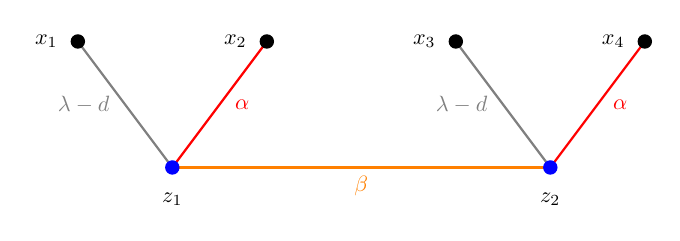
\begin{tikzpicture}[scale=0.8, every node/.style={transform shape}]
	%% vertex labels
	\node (z1) at (1.5,0) {};
	\node (Z1) at (1.5,-0.5) {$z_1$};
	\node (x1) at (0,2) {};
	\node (X1) at (-0.5,2) {$x_1$};
	\node (x2) at (3,2) {};
	\node (X2) at (2.5,2) {$x_2$};
	
	\node (z2) at (7.5,0) {};
	\node (Z2) at (7.5,-0.5) {$z_2$};
	\node (x3) at (6,2) {};
	\node (X3) at (5.5,2) {$x_3$};
	\node (x4) at (9,2) {};
	\node (X4) at (8.5,2) {$x_4$};

	\draw[color = gray, thick] (0,2) -- (1.5, 0) node [midway, left] {$\lambda-d \,\,$};
	\draw[color = red, thick] (1.5, 0) -- (3,2) node [midway, right] {$\,\,\alpha$};
	\draw[color = gray, thick] (6,2) -- (7.5,0) node [midway, left] {$\lambda-d\,\,$};
	\draw[color = red, thick] (7.5,0)
	-- (9,2) node [midway, right] {$\,\,\alpha$};
	\draw[color = orange, thick]  (1.5,0) -- (7.5,0) node [midway,below] {$\beta$};
	
	\draw[black, fill=black] (x4) circle (3pt);
	\draw[black, fill=black] (x3)  circle (3pt);
	\draw[black, fill=black] (x2)  circle (3pt);
	\draw[black, fill=black] (x1)  circle (3pt);
	\draw[blue, fill=blue] (z1) circle (3pt);
	\draw[blue, fill=blue] (z2) circle (3pt);
	
	\end{tikzpicture}
	\\
	Diagram $\tilde \Gamma$
\end{center}
The small scale degree on each edge of the tree graph is clearly greater than the dimension $-d$, so to apply Lemma~\ref{lem:diagram_integration}  we  only need to check the large scale condition is satisfied. Since 
$\cV_\ell  =\{\bullet_{x_1}, \bullet_{x_2}, \bullet_{x_3}, \bullet_{x_4}\}$,  
the tight partitions are :
$$\begin{aligned}
\P_1&=\{\cV_\ell, \{\bbullet_{z_1}\}, \{\bbullet_{z_2}\}\},  \qquad \P_2=\{\cV_\ell, \{\bbullet_{z_1},\bbullet_{z_2}\}\},  \\
\P_3&=\{ \{\cV_\ell, \bbullet_{z_1}\},\{\bbullet_{z_2}\}\},
\qquad  \P_4=\{ \{\cV_\ell, \bbullet_{z_2}\},\{\bbullet_{z_1}\}\}.
\end{aligned}
$$
A trivial computation shows that 
$$\begin{aligned}
\deg_\infty \, \P_1&=2\lambda -2d +2 \alpha +\beta +2d, \qquad \deg_\infty \, \P_2=2\lambda -2d +2 \alpha +d,\\
\deg_\infty \, \P_3&=\lambda -d + \alpha +\beta +d,
\end{aligned}$$
concluding the proof.
\end{proof}


\begin{lemma}\label{lem:diagram1_finite}
	For $F\in \Cc(\R^{4d})$ let
	\begin{equ} \label{eq:defn_I_Gamma1}
	I_{\Gamma_1}(F; \lambda)= \int_{\R^{8d}}
	\prod_{k=1}^4 |y_k - x_k|^{\lambda -d}  \, |y_1 - y_4|^{2-\kappa}
	|y_1- y_2|^{-\kappa} |y_3- y_4|^{-\kappa}  \, |F(x)|  \, 
	dx dy
	\end{equ}	
	\begin{equs} \label{eq:defn_I_Gamma2}
	&I_{\Gamma_2}(F; \lambda)= \int_{\R^{10d}} 
|y_1 - y_4|^{-\kappa}|z_1 - y_2|^{-\kappa} |z_2 - y_3|^{-\kappa} \\
 &\hspace{8em}
 |y_1 - z_1|^{\lambda - d}|y_4 - z_2|^{\lambda - d}\, 
\big(  \Pi_{i=1}^4 |x_i - y_i|^{\lambda - d}  \big) |F(x)|dy dz dx.	
\end{equs}
Then $I_{\Gamma_1}(F; \lambda)$ is finite for any $\lambda \in (0,\frac {3\kappa -2} 4)$;  and 
$I_{\Gamma_2}(F; \lambda)$ is finite for any $\lambda \in (0,\frac {\kappa } 2)$.\end{lemma}
\begin{proof}
	 The diagram associated to the integral is $\Gamma_1$ below, with the label indicating the
	 edge kernel degrees $\deg_0$ (which equals also $\deg_\infty$).
\begin{center}
	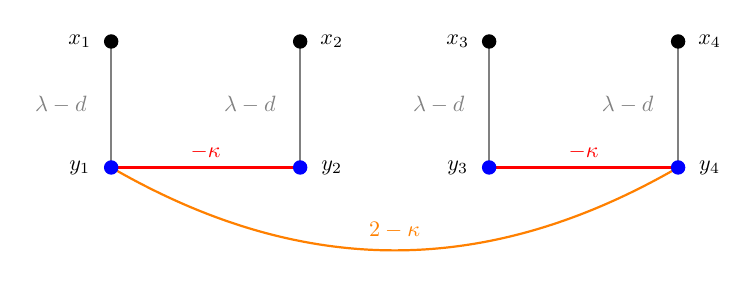
\begin{tikzpicture}[scale=0.8, every node/.style={transform shape}]
	%% vertex labels
	\node at (-0.5,0) {$y_1$};
	\node at (3.5,0) {$y_2$};
	\node at (-0.5,2) {$x_1$};
	\node at (3.5,2) {$x_2$};
	%
	\node at (5.5,0) {$y_3$};
	\node at (9.5,0) {$y_4$};
	\node at (5.5,2) {$x_3$};
	\node at (9.5,2) {$x_4$};
	
	% side vertical edges 
	\node at (-0.8, 1) { \textcolor{gray}{$\lambda -d$}};
	\node at (2.2, 1) { \textcolor{gray}{$\lambda -d$}};
	%
	\node at (5.2, 1) { \textcolor{gray}{$\lambda -d$}};
	\node at (8.2 , 1) { \textcolor{gray}{$\lambda -d$}};
	%
	\node at (4.5, -1) {\textcolor{orange}{$2-\kappa$}};
	
	%%% edges - left square
	\draw[color = red, thick] (0,0) -- (3,0) node [midway, above] {$-\kappa$};
	\draw[color = gray, thick] (0,0) -- (0,2);
	\draw[color = gray, thick] (3,0) -- (3,2);
	% right square
	\draw[color = red, thick] (6,0) -- (9,0) node [midway, above] {$-\kappa$};
	\draw[color = gray, thick] (6,0) -- (6,2);
	\draw[color = gray, thick] (9,0) -- (9,2);
	%% below
	\draw[color = orange, thick]  (0,0) to[out=-30,in=-150] (9,0);
	
	%% vertices
	\draw[blue, fill=blue] (0,0) circle (3pt);
	\draw[blue, fill=blue] (3,0) circle (3pt);
	\draw[fill=black] (0,2) circle (3pt);
	\draw[fill=black] (3,2) circle (3pt);
	%
	\draw[blue,fill=blue] (6,0) circle (3pt);
	\draw[blue, fill=blue] (9,0) circle (3pt);
	\draw[fill=black] (6,2) circle (3pt);
	\draw[fill=black] (9,2) circle (3pt);
	
	\end{tikzpicture}\\
	Diagram $\Gamma_1$
\end{center}


The integration simplifies after convolution / integrating out $y_2$ and $y_4$. For example,  under our conditions, 
$$ \int  |y_2 - x_2|^{\lambda -d} |y_1- y_2|^{-\kappa}	\;dy_2 = C|y_1-x_2|^{\lambda-\kappa}.$$
Then the integral is finite if and only if the integral associated with $\tilde \Gamma$ is finite where we take $\alpha = \lambda-\kappa$ and $\beta = 2-\kappa$, and we conclude the finiteness of the first integral by 
Lemma~\ref{lem:simple-graph}.
	The diagram associated to $I_{\Gamma_2}$ is as follows:	
\begin{center}
	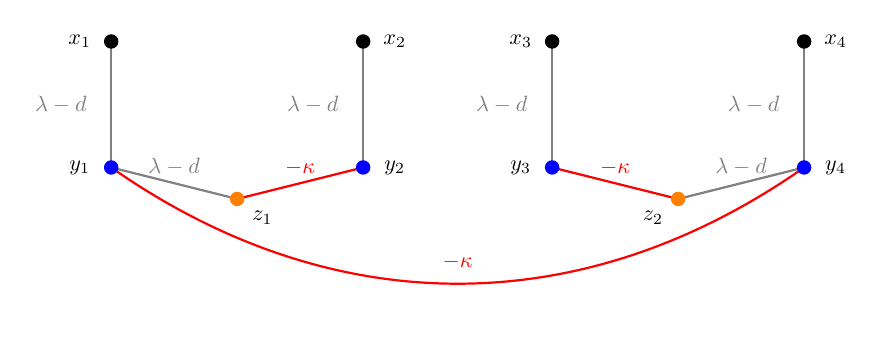
\begin{tikzpicture}[scale=0.8, every node/.style={transform shape}]
	%% vertex labels
	\node at (-0.5,0) {$y_1$};
	\node at (4.5,0) {$y_2$};
	\node at (-0.5,2) {$x_1$};
	\node at (4.5,2) {$x_2$};
	%
	\node at (6.5,0) {$y_3$};
	\node at (11.5,0) {$y_4$};
	\node at (6.5,2) {$x_3$};
	\node at (11.5,2) {$x_4$};
	%
	\node at (2.4,-0.8) {$z_1$};
	\node at (8.6,-0.8) {$z_2$};
	
	% side vertical edges 
	\node at (-0.8, 1) { \textcolor{gray}{$\lambda -d$}};
	\node at (3.2, 1) { \textcolor{gray}{$\lambda -d$}};
	%
	\node at (6.2, 1) { \textcolor{gray}{$\lambda -d$}};
	\node at (10.2 , 1) { \textcolor{gray}{$\lambda -d$}};
	%
	\node at (5.5, -1.5) {\textcolor{red}{$-\kappa$}};
	
	%%% edges - left square
	\draw[color = gray, thick] (0,0) -- (2,-0.5) node [midway, above] {$\lambda -d$};
	\draw[color = red, thick] (2,-0.5) -- (4,0) node [midway, above] {$-\kappa$};
	\draw[color = gray, thick] (0,0) -- (0,2);
	\draw[color = gray, thick] (4,0) -- (4,2);
	% right square
	\draw[color = gray, thick] (9,-0.5) -- (11,0)  node [midway, above] {$\lambda -d$};
	\draw[color = red, thick] (7,0) -- (9,-0.5)  node [midway, above] {$-\kappa$};
	\draw[color = gray, thick] (7,0) -- (7,2);
	\draw[color = gray, thick] (11,0) -- (11,2);
	%% below
	\draw[color = red, thick]  (0,0) to[out=-35,in=-145] (11,0);
	
	%% vertices
	\draw[blue,fill=blue] (0,0) circle (3pt);
	\draw[blue,fill=blue] (4,0) circle (3pt);
	\draw[fill=black] (0,2) circle (3pt);
	\draw[fill=black] (4,2) circle (3pt);
	\draw[orange,fill=orange] (2,-0.5) circle (3pt);
	%
	\draw[blue,fill=blue] (7,0) circle (3pt);
	\draw[blue,fill=blue] (11,0) circle (3pt);
	\draw[fill=black] (7,2) circle (3pt);
	\draw[fill=black] (11,2) circle (3pt);
	\draw[orange,fill=orange] (9,-0.5) circle (3pt);
	
	\end{tikzpicture}\\
	Diagram $\Gamma_2$
\end{center}
we again note that this graph reduces to $\tilde \Gamma$ where $\alpha = 2\lambda-\kappa$ and $\beta = -\kappa$
and apply Lemma~\ref{lem:simple-graph} to conclude.	\end{proof}

With these in place, we are going to recast the  bounds for $ \var( A_{1,\epsilon}) $ and for $ \| A_{2,\epsilon}\|_2$ 
in terms of the form $o(\epsilon) I_{\Gamma_i}$, where
$I_{\Gamma_i}$ were shown to be finite by analysing the associated Feynman diagrams. The main result of the section is:

\begin{proposition}\label{prop:vanishing_terms_bounds}
	Let $f, g \in \Cc(\R^d)$ and $\tau, v >0$. Then, for any given $\lambda$ in the region stated below, the following bounds hold uniformly  in $\epsilon \in (0,1)$:
\minilab{lemmaBound}\begin{equs}[2]
 \var( A_{1,\epsilon})  &\lesssim \epsilon^{\kappa -2} (\tau \wedge v)^{1-2\lambda} I_{\Gamma_1}(F; \lambda), \qquad
 & \lambda &\in (0,\tfrac 1 2)\;,\qquad\quad
 \label{eq:varA_1_control}\\
 \| A_{2,\epsilon}\|_2  &\lesssim \epsilon^{\frac \kappa 2 -1} (\tau\wedge v)^{\frac 3 2 (1-\lambda)} [ I_{\Gamma_2}(F; \lambda)]^{\frac 1 2}, \quad
 & \lambda &\in  [\tfrac 1 2, \tfrac 2 3);
 \label{eq:L2A_2_control}
\end{equs}
where $F=\prod_{i=1}^4 F_i$ where $F_i\in \{f,g\}$.
\end{proposition}
Note the integrals  $I_{\Gamma_i}(F; \lambda)$ are finite by Lemmas~\ref{lem:diagram1_finite}.
The proof of the proposition relies crucially on the bounds collected below in Lemma~\ref{lem:res_terms_estimates_multi} which, with $d$ in lieu of $\kappa$, are the same as in \cite[pp.~14--15]{gu20_nlmSHE}, up to rearranging, rescaling and integrating out the $x_i$ variables and upon setting $\tau = v$. In Lemma~\ref{lem:res_terms_estimates_multi} we added multi-time indices and test functions for clarity.
For this set
$dx = \prod_{i=1}^4 dx_i$, $dy = \prod_{i=1}^4 dy_i$, $dz = \prod_{i=1}^2 dz_i$,
and for  $f, g :\R^d\to \R$, set
 \begin{equation}
 \begin{aligned}
	\psi_{f,g}(x) &:= f(x_1) g(x_2) g(x_3)  f(x_4),\quad 
	\varphi_{f,g}(x) := f(x_1) g(x_2) f(x_3)  g(x_4),\\
		Q(x) &:= \int_0^\infty \int_{\R^{2d}} P_r(x - z_1) P_r(z_2) |R(z_1 -z_2)|\, dz\, dr.
\end{aligned}
	\end{equation}

\begin{lemma}\label{lem:res_terms_estimates_multi}
 For  any test functions $f, g :\R^d\to \R$, one has 
	\begin{equs}[2]	
	\var(A_{1, \epsilon})& \lesssim \sum_
	{\substack{i=1,2\\ j= 3,4}}
	\int_{0}^{\tau \wedge v} \int_{\R^{8d}} 
	\bigg(\prod_{k=1}^2  P_{ \tau -s} (y_k - x_k) P_{v -s} (y_{2+k} - x_{2+k})\bigg)  Q(\tfrac{y_i - y_j}{\epsilon}) 
	\\
	&  \hspace{1em}
	\epsilon^{-\kappa}\big|R(\tfrac {y_1- y_2} \epsilon)\big| \epsilon^{-\kappa}\big|R(\tfrac {y_3- y_4} \epsilon)\big| \, 	
	|\varphi_{f,g}(x)|  \, 
	dx dy ds,
\label{eq:varA1_estimate}\\
	\| A_{2, \epsilon} \|_2 &\lesssim \epsilon^{\frac \kappa 2 -1 } 	\int_{0}^{\tau \wedge v}  \bigg[ \int_s^{\tau} \int_{\R^{10d}} 
	P_{{\tau}-r} ( x_1 - y_1  ) P_{\tau-r} ( x_4 - y_4  )\\
	& \hspace{1em}  P_{r-s} ( y_1 - z_1 )  P_{r-s} ( y_4 - z_2 )  \,
	\epsilon^{-\kappa}\big|R(\tfrac {y_1- y_4} \epsilon)\big|
	\epsilon^{-\kappa}\big|R(\tfrac {z_1- y_2} \epsilon)\big|
	\epsilon^{-\kappa}\big|R(\tfrac {z_2 - y_3} \epsilon)\big|
	\\
	& \hspace{1em}  P_{{v}-s} ( y_2 - x_2) P_{{v}-s} ( y_3 - x_3) 	\,\big|\psi_{f,g}(x)\big| \,
	dy dz dx dr \bigg]^{\frac 1 2} ds,  \label{eq:A2_estimate}
	\end{equs}
	\end{lemma}


\begin{proof}
We follow \cite{gu20_nlmSHE} and begin with
	\begin{equ}
	\begin{aligned}
	\var (A_{1, \epsilon}) &= 
	\beta^2 \int_0^{\tau \wedge v}
	\int_{\R^{8d}} \epsilon^{-\kappa} R(\tfrac{y_1 -y_2}{\epsilon})  \epsilon^{-\kappa} R(\tfrac{y_3 -y_4}{\epsilon}) \,
	\cov\Big( \Lambda_\epsilon (s, y_1, y_2), \Lambda_\epsilon (s, y_3, y_4) \Big)   \\
	& \hspace{1em} 
	\prod_{k=1}^2 \bigg( P_{\tau -s} ( x_k - y_k ) P_{v-s } ( x_{k+2} - y_{k+2}) \bigg) 
	f(x_1) g(x_2) f(x_3)  g(x_4)  \, dx  dy ds
	\end{aligned}
	\end{equ}
	where $
	\Lambda_\epsilon (s, y_1, y_2) := 
	 \sigma(u(\tfrac s {\epsilon^2}, \tfrac {y_1} \epsilon))
	 \sigma(u(\tfrac s {\epsilon^2}, \tfrac {y_2} \epsilon))$.
By the Clark--Ocone formula, 
	\begin{equ}
	\begin{aligned}
	\cov\Big( \Lambda_\epsilon (s, y_1, y_2), \Lambda_\epsilon (s, y_3, y_4) \Big) &= 
	 \int_0^{\frac s {\epsilon^2}}
	\int_{\R^{2d}} R(z_1 -z_2)  \,\E \Big[ \E [ D_{r,z_1} \Lambda_\epsilon (s, y_1, y_2) | \F_r|]   \\
	& \hspace{4em} \times \E [ D_{r,z_2} \Lambda_\epsilon (s, y_3, y_4) | \F_r|]  \Big]  dz dr.
	\end{aligned}
	\end{equ}
	Using the chain rule to expand $D_{r,z} \Lambda_\epsilon (s, y_1, y_2)$ and the  bounds \eqref{eq:moment_Du}-\eqref{eq:moment_sigma_u}, 
	\begin{equ}\label{eq:est_D_Lambda}
	\| D_{r,z_1} \Lambda_\epsilon (s, y_1, y_2) \|_2 \lesssim P_{\frac s {\epsilon^2} -r} (\tfrac {y_1} \epsilon - z) + P_{\frac s {\epsilon^2} -r} (\tfrac {y_2} \epsilon - z). 
	\end{equ}
	Then, we have
	\begin{equ}\label{eq:bound_cov_Lambda}
	\left| \cov\Big( \Lambda_\epsilon (s, y_1, y_2), \Lambda_\epsilon (s, y_3, y_4) \Big) \right| \lesssim \sum_
	{\substack{i=1,2\\ j= 3,4}} Q(\tfrac{y_i - y_j}{\epsilon}),
	\end{equ}
thus concluding \eqref{eq:varA1_estimate}. 		
Similarly, using Minkowski inequality,
\begin{equs}%\label{eq:l2momentA2_B_est}
	\| A_{2,\epsilon}\|_2 & \leq \epsilon^{-d} \int_{0}^{\tau\wedge v} \bigg(
\int_{\R^{8d}} 
B_\epsilon^{\tau} (s, x_1, x_1', y_1, y_1', y_2, y_2')
P_{v-s} (x_2 -y_2) P_{v-s} (x_2' -y_2') \\
& \hspace{2em}\epsilon^{-\kappa} \big| R(\tfrac{y_1 -y_2}{\epsilon})\big| \epsilon^{-\kappa} \big|R(\tfrac{y_1' -y_2'}{\epsilon})\big| f(x_1) g(x_2) f(x_1') g(x_2') dx dx' dy dy'
\bigg)^{\frac 1 2} ds, \qquad \hbox{where}\\
&B_\epsilon^{\tau} (s, x_1, x_1', y_1, y_1', y_2, y_2') 
	= \E \Big[ \tilde{A}^{\tau}_{2, \epsilon} ( x_1, \tfrac s \epsilon, \tfrac {y_1} \epsilon)
	\tilde{A}^{\tau}_{2, \epsilon} ( x_1', \tfrac s \epsilon, \tfrac {y_1'} \epsilon)
	 \sigma(u_\epsilon(s, y_2)) 
	\sigma(u_\epsilon(s, y_2')) 
	\Big].
\end{equs}
	Recalling the definition \eqref{eq:defn_A2-tilde} of $\tilde{A}^\tau_{2, \epsilon}$,	
	 first apply It\^{o} isometry, then estimate via H\"{o}lder inequality and the
	 moment bounds on $Du$, $\sigma(u)$ from Lemma~\ref{lem:moments}, and finally perform a change of variables,
	\begin{align*}
	& |B_\epsilon^{\tau} (s, x_1, x_1', y_1, y_1', y_2, y_2')  | 
	\\
	& = 
	\bigg|  
	\int_{\frac s {\epsilon^2}}^{\frac \tau {\epsilon^2}} \int_{\R^{2d}} \E \big[
	\Sigma(r,z_1) \Sigma(r,z_2)  D_{\frac s {\epsilon^2}, \frac {y_1} \epsilon} u(r,z_1)
	D_{\frac s {\epsilon^2}, \frac {y_1'} \epsilon} u(r,z_2) \sigma(u(\tfrac s {\epsilon^2}, \tfrac {y_2} \epsilon )) \sigma(u(\tfrac s {\epsilon^2}, \tfrac {y_2'} \epsilon ))
	\big] \\
	& \hspace{4em} P_{\frac \tau {\epsilon^2} - r}  (\tfrac{x_1}{\epsilon} - z_1) 
	P_{\frac \tau {\epsilon^2} - r}  (\tfrac{x_1'}{\epsilon} - z_2) R(z_1 -z_2)\, dz dr
	\bigg|\\
	& \lesssim 
	\int_{\frac s {\epsilon^2}}^{\frac \tau {\epsilon^2}} \int_{\R^{2d}}  
	P_{r-\frac s {\epsilon^2} }  (z_1-\tfrac{y_1}{\epsilon}) P_{r- \frac s {\epsilon^2}}  (z_2-\tfrac{y_1'}{\epsilon} )
	 P_{\frac \tau {\epsilon^2} - r}  (\tfrac{x_1}{\epsilon} - z_1) 
	P_{\frac \tau {\epsilon^2} - r}  (\tfrac{x_1'}{\epsilon} - z_2)\big| R(z_1 -z_2)\big|\, dz dr
	\\
	& = \epsilon^{\kappa-2+2d} \int_{ s }^{\tau} \int_{\R^{2d}}  
	P_{r-s}  (z_1-{y_1}) P_{r - s}  ( z_2 - {y_1'} )
	P_{\tau - r}  ({x_1} - z_1) 
	P_{\tau - r}  ({x_1'} - z_2) \epsilon^{-\kappa} \big|R(\tfrac {z_1 -z_2} \epsilon)\big|\, dz dr.
	\end{align*}
	Returning to estimate for $\| A_{2,\epsilon}\|_2$ and relabelling integrating variables\footnote{Namely, we relabel $(x_1, x_1', x_2, x_2')$ with $(x_1, x_4, x_2, x_3)$, and $( z_1, z_2, y_1, y_1', y_2, y_2')$ with $( y_1, y_4, z_1, z_2, y_2, y_3)$.} to conclude~\eqref{eq:A2_estimate}.
\end{proof}




\subsubsection*{Proof 
	of Proposition~\ref{prop:vanishing_terms_bounds}}

We begin proving \eqref{eq:varA_1_control}.
Since $\epsilon^{-\kappa} |R(\tfrac{x}{\epsilon})| \lesssim |x|^{-\kappa}$, and by Lemma~\ref{lem:gaussian_cov_est},  we see that
\begin{equ}
Q(\tfrac{x}{\epsilon}) \lesssim  1 \wedge \epsilon^{\kappa -2}  |x|^{2-\kappa} \lesssim \epsilon^{\kappa -2}  |x|^{2-\kappa}. 
\end{equ}
Plugging these estimates into \eqref{eq:varA1_estimate} and bringing time integral inside, we have 
\begin{align*}
\var(A_{1, \epsilon})& \lesssim \epsilon^{\kappa -2}  \sum_
{\substack{i=1,2\\ j= 3,4}}
\int_{\R^{8d}}   \bigg(
\int_{0}^{\tau \wedge v} \prod_{k=1}^2  P_{\tau-s} (y_k - x_k) P_{v-s} (y_{2+k} - x_{2+k}) ds  \bigg)  
\\
&  \hspace{3em}
|y_i - y_j|^{2-\kappa} |y_1- y_2|^{-\kappa} |y_3- y_4|^{-\kappa}  \, 	|\varphi_{f,g} (x)|
dx\, dy\, ds.
\end{align*}
Let $t = \tau \wedge v$ and $\lambda \in (0, \frac 1 2)$. We use again the pointwise estimate \eqref{eq:comp_est} from Lemma~\ref{lem:gaussian_time_bounds}. For $r \in \{ \tau, v\}$, we have $r \geq t$, so that $P_{r-s} (x) \lesssim  (t-s)^{-\frac \lambda 2} |x|^{\lambda - d}$ uniformly in $t, s$ and $x \neq 0$. Hence, we estimate as follows
\begin{align*}
\var(A_{1, \epsilon})& \lesssim \epsilon^{\kappa -2}  \sum_
{\substack{i=1,2\\ j= 3,4}}
\int_{\R^{8d}}   \bigg(
\int_{0}^{t} (t-s)^{-2\lambda} \, ds  \bigg)    
\prod_{k=1}^4 |y_k - x_k|^{\lambda -d}  
\\
&  \hspace{2em}
|y_i - y_j|^{2-\kappa} \, 
|y_1- y_2|^{-\kappa} |y_3- y_4|^{-\kappa}  \, 	|\varphi_{f,g}(x)|  \, 
dx dy ds \\
&=\epsilon^{\kappa -2}  t^{1-2\lambda} \sum_
{\substack{i=1,2\\ j= 3,4}}
\int_{\R^{8d}}   \bigg(
\prod_{k=1}^4 |y_k - x_k|^{\lambda -d}   \bigg)
|y_i - y_j|^{2-\kappa} \\
&  \hspace{10em}
|y_1- y_2|^{-\kappa} |y_3- y_4|^{-\kappa}  \, 	|\varphi_{f,g}(x)|  \, 
dx dy ds.
\end{align*}
Lemma \ref{lem:diagram1_finite} allows to  conclude $\var(A_{1, \epsilon}) \lesssim \epsilon^{\kappa -2} \, (\tau \wedge v)^{1-2\lambda}I_{\Gamma_1}(F; \lambda)$. 

We go ahead proving \eqref{eq:L2A_2_control}.
Since $\epsilon^{-\kappa} |R(\tfrac x \epsilon )| \lesssim |x|^{-\kappa}$, letting $t = v \wedge \tau$, from the bound of Lemma~\ref{lem:res_terms_estimates_multi} we have
\begin{equs}
\| A_{2, \epsilon} \|_2 &\lesssim \epsilon^{\frac \kappa 2 -1 } 	\int_{0}^{t}  \bigg[ \int_s^{\tau} \int_{\R^{10d}}  |\psi_{f,g}(x)| \,
P_{{\tau}-r} ( x_1 - y_1  ) P_{{\tau}-r} ( x_4 - y_4  ) \\
& \hspace{6em}  P_{r-s} ( y_1 - z_1 )  P_{r-s} ( y_4 - z_2 )  \,
|y_1 - y_4|^{-\kappa}|z_1 - y_2|^{-\kappa} |z_2 - y_3|^{-\kappa}  
\\
& \hspace{6em}  P_{{v}-s} ( y_2 - x_2) P_{{v}-s} ( y_3 - x_3) 
dy dz dx dr \bigg]^{\frac 1 2} ds.
\end{equs}
Applying Jensen's inequality (with respect to the normalised measure $\frac{ds}t$) and bringing time integrals inside, 
we have
\begin{equs}
\| A_{2, \epsilon} \|_2 
&\lesssim \epsilon^{\frac \kappa 2 -1 } \sqrt t  \bigg[  \int_{\R^{10d}} 
|\psi_{f,g}(x)| \, |y_1 - y_4|^{-\kappa}|z_1 - y_2|^{-\kappa} |z_2 - y_3|^{-\kappa} \\
& \qquad 
\bigg( \int_{0}^{t} P_{{v}-s} ( y_2 - x_2) P_{{v}-s} ( y_3 - x_3)  \int_s^{\tau} 
P_{{\tau}-r} ( x_1 - y_1  ) P_{{\tau}-r} ( x_4 - y_4  ) 
\\
& \qquad
P_{r-s} ( y_1 - z_1 )  P_{r-s} ( y_4 - z_2 )    
dr ds \bigg)
dy dz dx \bigg]^{\frac 1 2}.  
\end{equs}
We can now apply Lemma~\ref{lem:multiple_time_int} with some fixed $\lambda \in [\frac 1 2, \frac 2 3)$ to obtain
\begin{equs}
\| A_{2, \epsilon} \|_2 &\lesssim \epsilon^{\frac \kappa 2 -1 } t^{ \frac 3 2 ( 1- \lambda) } \bigg[  
\int_{\R^{10d}} |\psi_{f,g}(x)|   
|y_1 - y_4|^{-\kappa}|z_1 - y_2|^{-\kappa} |z_2 - y_3|^{-\kappa}
\\
& \qquad 
 |y_1 - z_1|^{\lambda - d}|y_4 - z_2|^{\lambda - d}\, 
\big(  \Pi_{i=1}^4 |x_i - y_i|^{\lambda - d}  \big) dy dz dx \bigg]^{\frac 1 2}
 =  \epsilon^{\frac \kappa 2 -1 } t^{ \frac 3 2 ( 1- \lambda) }  [I_{\Gamma_2} ]^\frac 1 2.
\end{equs}
This concludes the proof of the Proposition.

%%%%%%%%%%%%%%%
\section{Weak convergence of \TitleEquation{X^\epsilon}{X eps} in H\"{o}lder topology}\label{sec:weak_convergence}

We recall $\kappa \in (2, d)$ is the decay exponent of the spatial covariance $R$,
 $\cU_t(g)$ denotes the Edwards--Wilkison solution at time $t>0$ tested against a test function $g$, namely,
\begin{equ} 
\cU_t(g) 
= \beta \nueff  \int_0^t \int_{ \R^d} \bigg( \int_{ \R^d}
P_{t-s} (x-y) g(x) dx
\bigg) dW^\kappa (s,y),
\end{equ} 
where $W^\kappa$ is centred Gaussian noise with spatial covariance $|x|^{-\kappa}$.
Let us also recall 
\begin{equ}
X_{t}^{\epsilon, g} = \epsilon^{1-\f \kappa 2}\int_{\R^d}  \bigl( u_\epsilon(t,x)- 1\bigr)g(x) dx.
\end{equ}

In this section we show that  $X^\epsilon$ converges weakly to the Edwards--Wilkison solution $\cU$, as distribution valued stochastic processes with  H\"{o}lder continuous in time trajectories.
Throughout this section we let $\delta_0 := \frac 1 2 \wedge \frac{\kappa-2}{4}$.
The parameter $\delta < \delta_0$ will represent a (space-time) regularity trade-off factor, whereas $\gamma \in (0, \frac 1 2)$ will parametrise H\"{o}lder continuity in time and $\alpha < -1$ the distributional regularity. 



Let $\S^\prime = \S^\prime(\R^d)$ denote the space of tempered distributions consisting 
of continuous linear functional on the space of Schwartz test functions (rapidly decaying smooth functions) on $\R^d$.  Let $\eta$ denote a test function, not to be confused with the white noise in the beginning of the article, and for $x\in \R^d$ and $\lambda>0$ let $\eta^\lambda_x $ denote its transformation by scaling and translation:
 \begin{equ}
%\scal
\eta^\lambda_x (y) := \lambda^{-d} \eta ( \tfrac{y-x}{\lambda}).
\end{equ}
These operations are $L^1$ invariant. 
Let $\B^r_0$ denote the subset of $r$-H\"older continuous test functions with support in the unit ball and with $\C^r$ norm less or equal to 1:
$$  
\B^r_0 := \{ \eta \in \C^r: \supp(\eta)\subset B(0,1), \|\eta\|_{\C^r}\le 1 \}.
$$

We introduce notations concerning the spaces of negative H\"{o}lder regularity $\C^\alpha$, with $\alpha <0$. 
Let $ \lceil -\alpha \rceil$ be the smallest (positive) integer bigger than $-\alpha$.
 Let  $\C^\alpha \subset \S^\prime$ denote the subset of locally H\"older continuous distributions.   Following \cite[Defn 3.7]{hairer_RegStr},  a distribution  $\zeta $ is said to be in $ \C^\alpha$, if  
 for every compact set $E \subset \R^d$, there exists a constant $C_E$  such that for all 
 $\eta \in \C^{\lceil -\alpha \rceil}$,
 $\lambda \in (0,1)$ and  $x \in E$, the  scaling relation below holds:
\begin{equ}
\langle \zeta,  \eta^\lambda_x \rangle \leq C_E \lambda ^\alpha.
\end{equ}
 Letting $r = \lceil -\alpha \rceil $, we define  the  semi-norms:
\begin{equ}\label{eq:seminorm_Calpha_basic}
	\| \zeta \|_{\alpha; E} := \sup_{\eta \in \B^r_0 } \sup_{ \lambda \in (0,1)} \sup_{x \in  E}  \,\, \lambda^{-\alpha}| \langle \zeta, \eta^\lambda_x \rangle |.
\end{equ}
We can also pick weights with $\sum_{m=1}^\infty w(m) < \infty$, these can be chosen according to the growth of seminorms  $\|\zeta \|_{\alpha,B_m}$, where $B_m$ denotes the closed ball of radius $m$ centred at the origin. Then, one may define 
another distance on $\C^\alpha$, 
\begin{equ}\label{dw}
d_\alpha (\zeta, \zeta') \equiv d^w_{\alpha} (\zeta, \zeta') := \sum_{m \geq 1} w(m) \big(1 \, \wedge \, \| \zeta - \zeta' \|_{\alpha; B_m} \big).
\end{equ}
We often pick up $w_m=2^{-m}$ and use the metric given by
\begin{equ}\label{eq:metric_Calpha}
d_{\alpha} (\zeta, \zeta') := \sum_{m \geq 1} 2^{-m} \big(1 \, \wedge \, \| \zeta - \zeta' \|_{\alpha; B_m} \big).
\end{equ}


As metric spaces, $\C^{\alpha'}$ is compactly embedded in $\C^\alpha$ for any $\alpha' < \alpha$.\\

We state the main theorem, from which  Theorem~\ref{thm:weak_conv_1} follows.
\begin{theorem}\label{thm:weak_conv}
		Assume the assumptions on $\kappa$, $R$ and $\sigma$ of Theorem~\ref{thm:basic-convergence}. 
		Let $\delta \in (0, \delta_0)$.
	For any $ \gamma \in (0, \frac 1 2 - \delta)$ and $\alpha < 2\delta - \frac \kappa 2$, there exists $\beta_{\gamma,\alpha} = \beta(\alpha,\gamma, d, R, \sigma) >0$ such that for any $\beta <\beta_{\gamma,\alpha}$, $X^\epsilon$ converges weakly to $\cU$ in $\C^{\gamma}([0,T], \C^{\alpha})$ as $\epsilon \to 0$. 
	\end{theorem}


\begin{proof}
In the next section, in Proposition~\ref{prop:tightness}, we shall show that for sufficiently small $\beta < \beta_{\gamma,\alpha}$, 
$\{X^\epsilon, \epsilon \in (0, 1]\}$ is tight in $\C^\gamma( [0,T], \C^\alpha)$. 

Since $\C^\alpha \subset \D'$, the law of $\zeta \in  \C^\alpha $ is uniquely determined  by the marginal law of random vectors $(\zeta(g_1), \dots, \zeta(g_n))$,  where $\{g_i\}_{i=1, \dots, n} \subset \D$ is a finite collection of smooth compactly supported functions.  In Theorem~\ref{thm:basic-convergence}, we have shown that for $\beta < \beta_0(4) \wedge \beta_1$,
for any $0< t_1 \leq t_2 \leq \dots t_n \leq T$, any $\{ g_i \}_{i=1, \dots, n} \subset \D$, \begin{equ} 
( X^{\epsilon, g_1}_{t_1}, \dots, X^{\epsilon, g_n}_{t_n}) \Rightarrow  ( \cU_{t_1}(g_1), \dots, \cU_{t_n}(g_n)),
\end{equ}
as $\epsilon \to 0$,  in distribution. This identifies the limit of $\cU$ and concludes the proof.
\end{proof}

\subsection{Preliminaries}
The spaces $\C^\alpha$ can be characterised in terms of wavelets, but also in terms of a sequence of functions $\{\varphi_n\}$ constructed from a single well chosen test function $\rho \in \Ccinf(\R^d)$. The former can be found in Sec 3.1-3.2 \cite{hairer_RegStr}, below we follow \cite{friz-hairer2020course} to construct $\{\varphi_n\}$.

For a given $\alpha<0$, let $\rho \in \Ccinf( \R^d)$ be symmetric and compactly supported in the ball $B(0,1)$ of radius 1 with $\|\rho\|_{L^1}=1$, and such that 
\begin{equ}
\int_{ \R^d} x^m \rho (x) \, dx =0, \qquad 0 < |m| \leq -\alpha,
\end{equ} 
where $m = (m_1, \dots, m_d)$ is a $d$-dimensional multi-index. 

Given a function  $g:\R^d \to \R$, 
we denote by $g_x$ its translation by $x$,  and $g^\lambda$ is dilation, so $$g_x:=g(\cdot -x), \qquad 
g^\lambda_x:=\lambda^{-d}g( \ff{\cdot -x}\lambda),  \qquad g^\lambda =\lambda^{-d}g( \ff \cdot \lambda).$$
But the notation $g^\lambda$ can be confused with its composition with the power function, so we we would use
$g^{(\lambda)}$ from time to time.

\begin{lemma} \cite[Lemma~13.24]{friz-hairer2020course} \label{lem:C^alpha_analytic} Let $\rho^{(n)} = 2^{nd} \rho (2^n \cdot) $.
	Suppose $\zeta_n : \R^d \to \R$ is a sequence of functions such that 
	\begin{enumerate}
		\item $\zeta_n = \zeta_{n+1} \ast \rho^{(n)}$,
		\item  there exists $\alpha <0$ such that  for any compact $E$, $\sup_{x \in E} |\zeta_n(x)| \leq C_E 2^{-\alpha n}$.
	\end{enumerate}
	Then, for any $\alpha' < \alpha$ the sequence $\zeta_n$ is Cauchy in $\C^{\alpha'}$ and converges to a unique $\zeta \in \C^{\alpha'}$. Furthermore $\zeta_n = \zeta \ast \rho^{(n)}$ and $\| \zeta \|_{\alpha', E} \lesssim C_E$. 
\end{lemma}


To apply this lemma, we construct $\zeta_n $ from a distribution $\zeta$. For this set 
\begin{equ}
\rho^{(n,m)} = \rho^{(n)} \ast \rho^{(n+1)}\ast \cdots  \ast \rho^{(m)}.
\end{equ}
Since $\rho^{(n+1)}=(\rho^{(1)})^{(n)}=(\rho^{(n)})^{(1)}$, convolution and scaling commute,  $ f\mapsto \rho^{(n)}*f$ is bounded in $\C^\alpha$ with uniform norm,  $\{\rho^{n,m}: m \ge 1\}$  is a Cauchy sequence. Set 
$$\varphi=\lim_{m\to \infty}\rho*\rho^{(1)}\dots *\rho^{(m)}, \qquad \qquad 
\tilde \varphi^{(n)} = \lim_{m \to \infty} \rho^{(n,m)}.$$
Then if $\varphi^{(n)}=2^{nd}\varphi(2^n \cdot)$, we have that
\begin{equ}\label{eq:prop_varphi_rho_n}
\tilde \varphi^{(n)} =\varphi^{(n)}, \qquad \varphi^{(n)} = \rho^{(n)} \ast \ \varphi^{(n+1)}, \quad\quad  \supp  \varphi^{(n)} \subset B(0, 2^{1-n}). 
\end{equ}
Finally we set $$
\zeta_n(x) = \langle \zeta , \varphi^{(n)}_x \rangle.$$
 Then Lemma~\ref{lem:C^alpha_analytic} provides an analytic criterion 
to establish  $\zeta \in \C^\alpha$ and quantify its seminorm $C_E$ for each compact $E$.  An immediate consequence is a method  for estimating the $\C^\alpha$ semi-norms of a random tempered distribution. 



\begin{lemma}\label{lem:random_C^alpha}
	Assume $ p\geq1$, $\alpha < 0$ and $\zeta$ is a random tempered distribution.  Let  $\varphi=\lim_{m\to \infty}\rho*\rho^{(1)}\dots *\rho^{(m)}$. 
	
	If for any compact $E$ there exists a constant $C_E$ (uniform in $n$) such that
	\begin{equ} \label{eq:moment_cond_Calpha_crit}
	\norm{\sup_{x \in E} |\langle \zeta , \varphi^{(n)}_x \rangle|}_p \leq C_E 2^{-\alpha n},
	\end{equ}
	then, for any $\alpha' < \alpha$,  $\zeta \in \C^{\alpha'}$ almost surely and $\Big\| \|\zeta \|_{\alpha', E} \Big\|_p \leq \sum_{n =1}^\infty  2^{(\alpha' - \alpha)n} C_{E}$. 
\end{lemma}
\begin{proof}
	Let $\zeta_n(x) = \langle \zeta , \varphi^{(n)}_x \rangle$, then
	$
	\zeta_n (x) =
	\langle \zeta ,  \varphi^{(n+1)} \ast \rho^{(n)}_x \rangle  = \zeta_{n+1} \ast \rho^{(n)} (x)$, and satisfies
 condition $(ii)$ of Lemma \ref{lem:C^alpha_analytic} almost surely by the assumption. Moreover, 	
 \begin{equ}	\norm{\|\zeta \|_{\alpha', E}}_p
	 = \norm{\sup_{n \geq 1} \,  \sup_{x \in E} 2^{\alpha'n} |\zeta_n(x)|  }_p 
	 \leq \sum_{n \geq 1} 2^{(\alpha' - \alpha)n}  \norm{\sup_{x \in E} 2^{\alpha n} |\zeta_n(x)|}_p,  
	\end{equ} concluding the proof.
\end{proof}


Let us now define the space of tempered distribution valued processes with lattice and spatial H\"{o}lder regularity controlled  when tested against functions $\varphi^{(n)}$. 

\begin{definition}\label{dis-class}
	A tempered distribution valued stochastic process $\zeta_t$ is said to belong to $\C^{\gamma_0, \alpha_0}_p$, with respect to the $L^{p}(\Omega)$ norm, if there exists $C>0$ such that the following estimates hold  for any compact set $E\subset \R^d$, $n\geq 1$ and $t,r \geq 0$,
	\begin{align}
	\label{eq:lattice+time_control-app}
	\sup_{x \in  E \cap 2^{-n}\mathbb{Z}^d} 
	\norm{\langle \zeta_{r,t}, \varphi^{(n)}_x \rangle }_{p} &\leq C 2^{-n\alpha_0} |t-r|^{\gamma_0}, \\
	\label{eq:spatial_control-app}
	\sup_{\substack{x\neq y \in  E,\\
			|x-y|\leq 2^{\frac d 2 -n}}}  
	\norm{\langle \zeta_{r,t}, \varphi^{(n)}_x - \varphi^{(n)}_y \rangle }_{p} &\leq C 2^{-n(\alpha_0-1)} |t-r|^{\gamma_0} |x-y|,
	\end{align}
	where $\zeta_{r,t} = \zeta_t - \zeta_r$. Let the smallest such constant $C$ be denoted by $\|\zeta\|_{\C^{\gamma_0, \alpha_0}_p}$.
\end{definition}
With this definition,  when the weights $w(m)$ are chosen appropriately, Proposition \ref{prop:time-holder_distribution_process-app}  asserts that  $\C^{\gamma_0, \alpha_0}_p$ can be embedded in $L^p(\Omega, \C^{\gamma_0-\frac 1 p -} ( [0,T], \C^{\alpha_0 - \frac d p -}))$.


\begin{proposition}\label{prop:time-holder_distribution_process-app}
	Let $\alpha_0<0$, $p > d$,  $\gamma_0 > \frac 1 {p}$, and $\zeta \in \C^{\gamma_0, \alpha_0}_p$. The following holds.
	\begin{itemize}
	\item [1.] For any compact set $E$, any $\alpha < \alpha_0 - \frac d p$,
	\begin{equ}\label{eq:moment_sup_compact-app}
	\norm{\sup_{x \in E} |\langle \zeta_{r,t}, \varphi^{(n)}_x \rangle|}_p \leq c \|\zeta\|_{\C^{\gamma_0, \alpha_0}_p} ( {\sqrt 2}^{\mu  d } + \diam(E)^{\frac 1 {p}}  )
	2^{-n \alpha} |t-r|^{\gamma_0},
	\end{equ}
	where $c$ is a universal constant and $\mu=1-(\alpha_0-\alpha)$.
\item[2.] Let $w(m)$ be numbers satisfying
	\begin{equ}\label{eq:weight_finite_app}
	 \sum_{m=1}^\infty   ( 2^{\mu \frac d 2} + \diam(B_m)^{\frac 1 {p}}  )w(m) < \infty.
	\end{equ}
	Then for any 
	$\gamma < \gamma_0  - \frac 1 p$, $\zeta $ belongs to $ \C^\gamma ([0,T], \C^\alpha)$ almost surely and 
	\begin{equ}\label{eq:holder_norm_p_momoment-app}
	\norm{ \| \zeta \|_{\C^\gamma ([0,T], \C^\alpha)}  }_p = \norm{    \sup_{t\neq r \in [0,T]}
		\frac { d_\alpha (\zeta_t, \zeta_r)} {|t-r|^\gamma}}_p \lesssim \|\zeta\|_{\C^{\gamma_0, \alpha_0}_p}.
	\end{equ}
	where $d_\alpha$ denotes the distance given by (\ref{dw}).
\end{itemize}
\end{proposition}


\begin{proof} Fix $n \geq 1$, $p$, and $r,t$ and set $\zeta^{(n)}_{r,t}(x) = \langle \zeta_{r,t} , \varphi^{(n)}_x \rangle$.
One can control the $p$-th moments over lattice points $E_n := E \cap 2^{-n} \mathbb{Z}^d$:
	\begin{equation}
	\E \big[ \sup_{x \in  E_n}  | 
	\zeta^{(n)}_{r,t}(x)
	|^p \big]^{\frac 1 p}  
	\leq \E \big[ \Sigma_{x \in E_n} | \zeta^{(n)}_{r,t}(x) |^{p} \big]^{\frac 1 {p}} 
	 \leq (\#E_n)^{\frac 1 {p}} \sup_{x \in  E_n} \E \big[ | \zeta^{(n)}_{r,t}(x) |^{p} \big]^{\frac 1 {p}}. 
	\end{equation}
Since $\# E_n \leq \diam(E)^d 2^{nd}$,   \eqref{eq:lattice+time_control-app} leads to
	\begin{equ}\label{eq:estimate_sup_lattice-app}
	\norm{\sup_{x \in  E_n}  |\zeta^{(n)}_{r,t}(x)|}_p \leq 
	\diam(E)^{\frac d {p}} \, 2^{n\frac d {p}}\,  \|\zeta\|_{\C^{\gamma_0, \alpha_0}_p} 2^{-n\alpha_0} |t-r|^{\gamma_0}.
	\end{equ}
	For any $x \in E$, we can find $z_n \in E_n$ such that $|x -z_n| \leq 2^{\frac d 2} 2^{-n}$, so for any $\mu>0$, 	\begin{equ}
	\begin{aligned}
	| \zeta^{(n)}_{r,t}(x)| & \leq | \zeta^{(n)}_{r,t}(x) -  \zeta^{(n)}_{r,t}(z_n)| + \sup_{ z \in E_n}  | \zeta^{(n)}_{r,t}(z)|  \\
	& \leq (2^{ \frac d 2} 2^{- n})^\mu \sup_{\substack{x\neq y \in  E,\\
			|x-y|\leq 2^{\frac d 2 -n}}} \frac { |  \zeta^{(n)}_{r,t}(x) - \zeta^{(n)}_{r,t}(y)|} {|x-y|^\mu }  +
	\sup_{ z \in E_n}  | \zeta^{(n)}_{r,t}(z)|. 
	\end{aligned} 
	\end{equ}
	On the other hand, for any $\mu<1-\f dp$, ther exists a constant $c$ such that 
  \begin{equ}\label{eq:kolmogorov_space-app}
	\norm{ \sup_{x\neq y \in  E} \frac { | 
			\zeta^{(n)}_{r,t}(x) - \zeta^{(n)}_{r,t}(y)	|} {|x-y|^\mu }}_{p} 
			\leq c \|\zeta\|_{\C^{\gamma_0, \alpha_0}_p}  \,2^{-n(\alpha_0-1)} |t-r|^{\gamma_0}.
	\end{equ}
	This follows easily from Kolmogorov's continuity theorem and the assumption \eqref{eq:spatial_control-app}. 
	Taking the supremum over $x \in E$ in the the estimate for $| \zeta^{(n)}_{r,t}(x)|$ and combining \eqref{eq:kolmogorov_space-app} and \eqref{eq:estimate_sup_lattice-app},  we can estimate the $p$-th moments as follows 
	\begin{equ}
	\begin{aligned}
	\norm{\sup_{x \in  E}  |\zeta^{(n)}_{r,t}(x)|}_p  &\leq 
	(2^{\mu \frac d 2} 2^{-\mu n}  \, c  \,2^{-n(\alpha_0 -1)}     +  \diam(E)^{\frac d {p}} \, 2^{n\frac d {p}}\,  
	  2^{-n\alpha_0} )
	 \|\zeta\|_{\C^{\gamma_0, \alpha_0}_p} |t-r|^{\gamma_0}
	 \\
	& \leq c \|\zeta\|_{\C^{\gamma_0, \alpha_0}_p} ( 2^{\mu \frac d 2} + \diam(E)^{\frac 1 {p}}  )
	2^{-n \, (\alpha_0 - 1 + \mu) \wedge (\alpha_0 - \frac d {p})} |t-r|^{\gamma_0}.
	\end{aligned}
	\end{equ} 
	For any $\alpha < \alpha_0 - \frac d p$ we can pick $\mu = 1 -( \alpha_0-\alpha)$, so that
	\begin{equ}
	\norm{\sup_{x \in  E}  |\zeta^{(n)}_{r,t}(x)|}_p  \leq c \|\zeta\|_{\C^{\gamma_0, \alpha_0}_p} ( 2^{\mu \frac d 2} + \diam(E)^{\frac 1 {p}}  ) \;2^{-n \alpha} |t-r|^{\gamma_0}.
	\end{equ}
	We can now apply Lemma \ref{lem:random_C^alpha} to obtain
		\begin{equ} 
	\norm{\|\zeta_{r,t} \|_{\alpha, E} }_p \leq c \|\zeta\|_{\C^{\gamma_0, \alpha_0}_p} ( 2^{\mu \frac d 2} + \diam(E)^{\frac 1 {p}}  )\;
	|t-r|^{\gamma_0}.
	\end{equ}
	Then, since the weights decay fast enough such that \eqref{eq:weight_finite_app} holds, we have
	\begin{align*}
	\norm{d_\alpha (\zeta_t, \zeta_r)}_p &\leq 
	\sum_{m \geq 1} w(m) \big(1 \, \wedge \, \norm{ \|  \zeta_t - \zeta_r \|_{\alpha; B_m}}_p \big) \\
	&\leq  c  \|\zeta\|_{\C^{\gamma_0, \alpha_0}_p} \sum_{m \geq 1} w(m)( 2^{\mu \frac d 2} + \diam(B_m)^{\frac 1 {p}}  ) \; |t-r|^{\gamma_0} \lesssim  |t-r|^{\gamma_0}. 
	\end{align*}
	Finally, for any $\gamma < \gamma_0 - \frac 1 p$ we can apply  Kolmogorov's continuity theorem to obtain \eqref{eq:holder_norm_p_momoment-app} and conclude $\zeta \in \C^{\gamma} ([0,T], \C^\alpha)$ almost surely, for any $T >0$.  
\end{proof}

 We now immediately have the following tightness criterion. 

\begin{proposition}[Tightness criterion]\label{prop:tightness-general}
Let $(\zeta^k)_{k \in \mathcal{I}}$ be a family of tempered distribution valued stochastic processes. Let $\alpha_0<0$, $p > d$,  $\gamma_0 > \frac 1 {p}$, and $\zeta \in \C^{\gamma_0, \alpha_0}_p$ with $\sup_k\|\zeta^k\|_{\C^{\gamma_0, \alpha_0}_p} <\infty$. Then $(\zeta^k)_{k \in \mathcal{I}}$ is tight in $\C^\gamma([0, T], \C^\alpha)$, for any $T >0$, any $\alpha < \alpha_0 - \frac d p$ and any $ \gamma < \gamma_0 - \frac 1 p$.
\end{proposition}

\begin{proof} We can take $w_m=2^{-m}$.
Firstly we note that $\C^{\gamma'}([0,T], \C^{\alpha'})$ is compactly embedded in $\C^{\gamma}([0,T], \C^{\alpha})$ for any $0< \gamma' < \gamma$, $\alpha' < \alpha$. We have $ \zeta^k \in \C^{\gamma}([0,T], \C^{\alpha}) $ with uniform  bound 
\begin{equ}
\sup_{k \in \mathcal{I}} \norm{    \sup_{t\neq r \in [0,T]}
	\frac { d_\alpha (\zeta^k_t, \zeta^k_r)} {|t-r|^\gamma}}_p \lesssim C,
\end{equ}
which is a consequence of Proposition \ref{prop:time-holder_distribution_process-app}, given $\zeta^k  \in \C^{\gamma_0, \alpha_0}_p$ with uniform constant $C$. Then tightness follows, as in the proof of Proposition \ref{prop:tightness},
\end{proof}


\subsection{Some elementary estimates}

For any $g \in \C^{1}_c$, set $g^\lambda =  \lambda^{-d} g(\frac \cdot \lambda)$.
To decompose and estimate the time increments of $X^\epsilon$ we consider
\begin{equ}\label{eq:defnIA_IB}
\begin{aligned}
I_A(r,t) &= \int_{r}^{t} \int_{\R^{2d}} \Pi_{i=1}^2 \bigg( \int_{\R^{d}} P_{t-s} (x_i - y_i) 
g^\lambda(x_i) dx_i \bigg) |y_1 - y_2|^{-\kappa} dy ds, \\
%
I_B(r,t) &= \int_0^{r} \int_{\R^{2d}} \Pi_{i=1}^2 \bigg( \int_{\R^{d}} ( P_{t-s} (x_i - y_i) - P_{r-s} (x_i - y_i)  ) 
g^\lambda(x_i) dx_i \bigg) |y_1 - y_2|^{-\kappa} dy ds,
\end{aligned}
\end{equ}
and bound them in terms of 
\begin{equ} 
\begin{aligned}
J_{\kappa, d- \tdelta} (f) &:= \int_{\R^{4d}} \bigg( \Pi_{i=1}^2 | f(x_i)| |x_i - y_i|^{\tdelta-d} \bigg) |y_1 - y_2|^{-\kappa} dy dx .   
\end{aligned}
\end{equ}
Since $\int_{\R^d} |x - y |^\alpha |y-w|^\beta dy = c_{\alpha, \beta} |w-x|^{\alpha + \beta +d}$, then for any bounded $f: \R^d\to \R^m$  with compact support with diameter $M$, there are constants $c$ and $C_{d,\tdelta, \kappa, M}$,
$$J_{\kappa, d- \tdelta} (f) = c\int |f(x_1)| | f(x_2)| |x_1-x_2|^{2\delta'-\kappa}\,dx\; \leq C_{d,\tdelta, \kappa, M} \| f\|_\infty ^2,$$
where the upper bound for the constant is of the form $M^{2d+2\delta'-\kappa}$. 
Note also that $$J_{\kappa, d - \delta'}( g^\lambda) = \lambda^{2\delta' - \kappa}J_{\kappa, d - \delta'}(g).$$



\begin{lemma}\label{lem:bounds_IAB}
	Let $\delta_0 = \frac 1 2 \wedge \frac{\kappa-2}{4}$. For any $\delta \in (0, \delta_0)$ there exists $C_\delta>0$ such that, for any
	$0\leq r <t$, 
%	 $0<\frac 2 3 t <r\leq t$, 
	 any $g \in \C^{1}_c$, and any $\lambda \in (0,1)$, \
	%$\frac 2 3 t <r\leq t$  
	%%	$t-r \leq \frac r 2$
	\begin{align}
	I_A(r,t) &\leq 
	C_\delta  \, |t -r|^{1  - 2\delta} \lambda^{4 \delta - \kappa  }  \,  J_{\kappa, d-2\delta} (g), \label{eq:est_IA}\\
	|I_B(r,t)| &\leq 
	C_\delta  \, |t -r|^{1  - 2\delta} \lambda^{4 \delta - \kappa  }  \,  \big(  J_{\kappa, d-2\delta} (g) + J_{\kappa, d-2\delta-1} (\nabla g) \big). \label{eq:est_IB} 
	\end{align}
	If $\delta < \frac{\kappa-2}{4}$, these are finite (The constants will blow up as $\delta$ approaches $0$ or  $\frac{\kappa-2}{4}$). 
	As a consequence,
	\begin{equ}\label{eq:est_IAB+}
	I_A(r,t) \lesssim   |t -r|^{1  - 2\delta} \lambda^{4 \delta - \kappa  }  \,   \| g\|_\infty ^2, \quad 
	|I_B(r,t)| \lesssim   |t -r|^{1  - 2\delta} \lambda^{4 \delta - \kappa  }  \,  \big(   \| g\|_\infty ^2 + \| \nabla g\|_\infty ^2\big),
	\end{equ}
	where the proportionality constants depend only on $d, \kappa, \delta$ and $\diam(\supp g)$.
\end{lemma}


\begin{proof}
	By change of time variable and then using the heat kernel estimate \eqref{eq:comp_est} with $\lambda = 2\delta$, 
	\begin{equs}
	I_A(r,t) &=  \int_{\R^{4d}}  \int_{0}^{t-r} \Pi_{i=1}^2  P_{s} (x_i - y_i) ds \, 
	\Pi_{i=1}^2  g^\lambda(x_i) |y_1 - y_2|^{-\kappa} dy dx \\
	&\lesssim \int_{0}^{t-r} s^{-2\delta} ds \, 
	\int_{\R^{4d}}   \Pi_{i=1}^2 \big(    |g^\lambda(x_i)| |x_i-y_i|^{2\delta -d }   \big) |y_1 - y_2|^{-\kappa} dy dx \\
	&= \tfrac{ 1}{1-2\delta} (t-r)^{1-2\delta} J_{\kappa, d - 2\delta}(g^\lambda)
	= \tfrac{ 1}{1-2\delta} (t-r)^{1-2\delta}  \lambda^{4\delta - \kappa}J_{\kappa, d - 2\delta}(g).
	\end{equs}
 	
	To estimate $I_B$,  we perform a change of time variable 
	\begin{equ}
	I_B(r,t) = \int_0^{r} \int_{\R^{2d}} \Pi_{i=1}^2 \bigg( \int_{\R^{d}} ( P_{t-r+s} (x_i - y_i) - P_{s} (x_i - y_i)  ) 
	g^\lambda(x_i) dx_i \bigg) |y_1 - y_2|^{-\kappa} dy ds, 
	\end{equ}
	and we consider separately two regions of integration: $[0, r_0]$ and $ [r_0, r]$ where $ r_0 := (t-r) \wedge \frac r 2$, so that  $|I_B| \leq I_B^{0, r_0} + I_B^{r_0, r}$ as introduced below. Using the brutal bound
	$\big|  P_{t-r + s} (x) - P_{s} (x)  \big|  \leq P_{t-r + s} (x) + P_{s} (x) \lesssim s^{-\delta} |x|^{2\delta-d} $ (again by \eqref{eq:comp_est} with $\lambda = 2\delta$), we have
	\begin{equ}
%	\label{eq:est_IB_term1}
	\begin{aligned}
	I_B^{0, r_0}(r,t) & := \int_0^{r_0} \int_{\R^{4d}}  \Pi_{i=1}^2 \big|  P_{t-r+s} (x_i - y_i) - P_{s} (x_i - y_i)  \big|  \Pi_{i=1}^2 |g^\lambda(x_i)| 
	|y_1 - y_2|^{-\kappa} \, dx dy ds \\
	&\lesssim  \int_0^{r_0}  s^{-2\delta} ds \, \int_{\R^{4d}} \Pi_{i=1}^2 |x_i -y_i|^{2\delta - d}  \,\Pi_{i=1}^2 |g^\lambda(x_i)| |y_1 - y_2|^{-\kappa} \, dx dy  \\
	& \leq \tfrac 1 {1- 2\delta} (t-r)^{1-2\delta} J_{\kappa, d-2\delta} ( g^\lambda) = \tfrac 1 {1- 2\delta} (t-r)^{1-2\delta} \lambda^{4\delta - \kappa} J_{\kappa, d-2\delta} (g).
	\end{aligned}
	\end{equ}
	For the integration over $s \in (r_0,r)$,
	\begin{equ}
	\begin{aligned}
	&\int_{\R^{d}} ( P_{t-r+s} (x-y) - P_{s} (x - y)  ) 
	g^\lambda(x) dx =\int_{\R^{d}} \int_{s}^{t-r+s} \partial_\tau  P_{\tau} (x-y) d\tau  g^\lambda(x) dx\\
	&\le \int_{\R^{d}} \int_{s}^{t-r+s} \big| \nabla_x P_{\tau} (x-y) \big| d\tau \,\,
	| \nabla ( g^\lambda(x))| dx    \\
	& \lesssim
	\int_{s}^{t-r+s} \tau^{-1-\delta}  d\tau \, \int_{\R^{d}} |x-y|^{1 +2\delta -d}
	| \nabla (  g^\lambda(x))| dx.
	\end{aligned}
	\end{equ}
	Then, we can now bound $I_B^{r_0, r}$, defined as follows:
	\begin{align*}
	&I_B^{r_0, r}(r,t):=  \\
	&\int_{r_0}^r \int_{\R^{2d}} \Pi_{i=1}^2 \bigg| \int_{\R^{d}} ( P_{t-r+s} (x_i - y_i) - P_{s} (x_i - y_i)  ) 
	g^\lambda(x_i) dx_i \bigg| |y_1 - y_2|^{-\kappa} dy ds  \\
	&\lesssim \int_{r_0}^r \bigg( \int_{s}^{t-r+s} \tau^{-1-\delta}  d\tau \bigg)^2 \, ds \,\, \times  \\
	& \hspace{8em} 
	\int_{\R^{4d}}
	\bigg( \Pi_{i=1}^2 |x_i-y_i|^{1 +2\delta -d}
	| \nabla ( g^\lambda(x_i))| \bigg) |y_1 - y_2|^{-\kappa}  dx dy. \\
	& = \delta^{-2}\int_{r_0}^r 
	\big( s^{-\delta}  - ( t-r + s)^{-\delta} \big)^2 ds \, \times \, J_{\kappa, d-2\delta -1}\big( \nabla ( g^\lambda)\big). 
	\end{align*} 
Since $\delta < \f 1 2$, 
we can bound 
\begin{align*}
&\delta^{-2} \int_{r_0}^r \big( s^{-\delta}  - ( t-r + s)^{-\delta} \big)^2 ds 
=\delta^{-2} (t-r)^{1-2\delta}\int_{\f {r_0} {t-r}}^{\f r {t-r}} (u^{-\delta}-(1+u)^{-\delta})^2 du\\
&\leq (t-r)^{1-2\delta}\;  \delta^{-2}\int_0^\infty
%\int_0 ^1
(u^{-\delta}-(1+u)^{-\delta})^2 du.
\end{align*}

Finally  	\begin{equ}%\label{eq:est_IB_term2}
	I_B^{r_0, r}(r,t)  \lesssim C_\delta (t-r)^{1-2\delta}\, \lambda^{4\delta -\kappa} J_{\kappa, d-2\delta -1}( \nabla g),
	\end{equ}
	and we collect estimates together to obtain \eqref{eq:est_IB}.
\end{proof}




\subsection{Tightness in \TitleEquation{\C^\gamma( [0,T], \C^\alpha)}{Cgamma([0,T],Calpha)}}

Given $t\geq  r \geq0$ set  $\cU_{r,t} =  \cU_t - \cU_r$ and $X^\epsilon_{r,t} =  X^\epsilon_t - X^\epsilon_r$. 
In the next two lemmas we gather together the time increments and spatial regularity bounds for $\cU$ and $X^\epsilon$, which allow us to identify, in  Proposition \ref{prop:time-holder_distribution_process-app},
suitable $\gamma \in (0,\frac 1 2)$ and $\alpha < -1$ such that the required tightness holds in $\C^\gamma( [0,T], \C^\alpha)$. 
 
  We note here that
 as $\delta$ approaches $0$ or $\frac{\kappa -2}{4}$, the implicit proportionality constant in the inequalities below blows up.
\begin{lemma}\label{lem:EW_cont_est}
	Let $p\geq 2$ and assume $\kappa \in (2, d)$. 
	For any $\delta \in (0, \delta_0)$ and any $g \in \C^{1}_c$,  
	we have the following bound for any 
	$0\leq r <t$, 
$x \in \R^d$ and $\lambda >0$, 
	\begin{equ}\label{eq:EW_cont_est_p}
	\| \cU_{r,t}( g^\lambda_x )    \|_p \lesssim   |t -r|^{\frac 1 2 -\delta} \lambda^{2\delta - \frac \kappa 2 }  \,\big( \|g\|_\infty + \|\nabla g\|_\infty   \big), 
	\end{equ}
	where the proportionality constant depends only on $d, \kappa, \delta$ and $\diam (\supp \, g)$. Moreover, if $g \in \C^{2}_c$, then 
	\begin{equ}\label{eq:EW_cont_est_p_spatial}
	\| \cU_{r,t}( g^\lambda_x - g^\lambda_y )    \|_p \lesssim   |t -r|^{\frac 1 2 -\delta} \lambda^{2\delta - \frac \kappa 2 -1}  \,\big( |g|_{Lip} + |\nabla g|_{Lip}   \big) |x-y|.
	\end{equ}
\end{lemma}
\begin{proof}
	By Gaussianity, it is sufficient to work with $p=2$.
	We have invariance in law under spatial translation $ \cU_t(g^\lambda_x) \stackrel{law}{=} \cU_t( g^\lambda)$, so we may focus only on test function $g^\lambda$. By It\^{o} isometry and decomposing the time interval $[0,  t] =  [ 0, r ]\cup [ r , t ]$, we can compute the second moment
	\begin{align*}
	&\| \cU_t( g^\lambda)  -   \cU_r( g^\lambda)    \|_2^2 \\ 
	& \quad = \beta^2 \nueff^2 \E \bigg( \int_{\R^{1+d}} 
	\int_{\R^d} \big( \1_{[0,t]}(s) P_{t-s} (x - y) - \1_{[0,r]}(s) P_{r-s} (x - y) \big)  g^\lambda(x) dx  \,  dW^\kappa(s,y) \bigg)^2 \\
	& \quad =\beta^2 \nueff^2 \big( I_A(r,t) + I_B(r,t) \big), 
	\end{align*}
	where $I_A$ and $I_B$ are defined in \eqref{eq:defnIA_IB} above. Hence, by taking square roots and plugging \eqref{eq:est_IAB+}, 
	\begin{equ}
	\| \cU_{r,t}(  g^\lambda)  \|_2 \lesssim 
	\beta \nueff \big( I_A(r,t) + I_B(r,t) \big)^{\frac 1 2} \lesssim 
	|t -r|^{\frac 1 2  - \delta} \lambda^{2 \delta - \frac \kappa 2  }  \,  \big(   \| g\|_\infty + \| \nabla g\|_\infty \big),
	\end{equ}  
	from which (\ref{eq:EW_cont_est_p}) follows. 	
	For \eqref{eq:EW_cont_est_p_spatial}, we note that $g^\lambda_x - g^\lambda_y = (g_{\frac x \lambda} - g_{\frac y \lambda})^\lambda$. Given $g \in \C^2_c$, we have
	$\| g_{\frac x \lambda} - g_{\frac y \lambda}\|_\infty \leq \lambda^{-1} |g|_{Lip} |x-y|$ and $\| \nabla (g_{\frac x \lambda} - g_{\frac y \lambda})\|_\infty \leq \lambda^{-1} |\nabla g|_{Lip} |x-y|$. Then 
	\begin{equ} 
	\| \cU_{r,t}( g^\lambda_x - g^\lambda_y)  \|_2  
	\lesssim 
	|t -r|^{\frac 1 2  - \delta} \lambda^{2 \delta - \frac \kappa 2 -1 }  \,  \big( |g|_{Lip}+ |\nabla g|_{Lip} \big) |x -y|,
	\end{equ}
	and \eqref{eq:EW_cont_est_p_spatial} follows. 
\end{proof}
\begin{lemma}\label{lem:X_cont_est}
	Under assumptions on $\kappa$, $R$ and $\sigma$ of Theorem~\ref{thm:basic-convergence}. 
Let $p \geq 2$ and $\beta < \beta_0(p)$.
For any $\delta \in (0, \delta_0)$ and any $g \in \C^{1}_c$, we have the following
 bound for any 
 	$0\leq r <t$, 
$x \in \R^d$ and $\lambda >0$, 
\begin{equ}\label{eq:Xeps_cont_est_p}
\sup_{\epsilon \in (0,1)} \| X_{r,t}^{\epsilon,  g^\lambda_x}  \|_p \lesssim   |t -r|^{\frac 1 2 -\delta} \lambda^{2\delta - \frac \kappa 2 }  \,\big( \|g\|_\infty + \|\nabla g\|_\infty   \big),
\end{equ}
where the proportionality constant depends only on $d, \kappa, \delta$ and $\diam (\supp \, g)$.
Moreover, if $g \in \C^{2}_c$, then 
\begin{equ}\label{eq:Xeps_cont_est_p_spatial}
\sup_{\epsilon \in (0,1)} \| X_{r,t}^{\epsilon,  g^\lambda_x-g^\lambda_y}  \|_p\lesssim   |t -r|^{\frac 1 2 -\delta} \lambda^{2\delta - \frac \kappa 2 -1}  \,\big( |g|_{Lip} + |\nabla g|_{Lip}   \big) |x-y|.
\end{equ}
\end{lemma}
\begin{proof}	Given spatial stationarity of $u_\epsilon(t,x)$, we only need to work with $ g^\lambda$, without the shifts. 	
Note that
	\begin{align*}
	&X_t^{\epsilon,  g^\lambda } - X_r^{\epsilon,  g^\lambda } = 
	\tfrac{\beta}{\epsilon^{\frac \kappa 2 -1}} \int_{\R^{d}} \big( u_\epsilon(t,x) - u_\epsilon(r,x)\big)  g^\lambda (x) dx = 
	\tfrac{\beta}{\epsilon^{\frac \kappa 2 -1}} \big( \A^{\epsilon}_{r, t} + \B^{\epsilon}_{r, t} \big),  \; \hbox{where}\\
	&\A^{\epsilon}_{r, t} =  \int_{\frac{r}{\epsilon^2}}^{\frac{t}{\epsilon^2}}
	\int_{\R^{d}} \sigma(u(s,y)) \int_{\R^{d}} P_{\frac{t}{\epsilon^2} -s}  (\tfrac{ x}{\epsilon} -y)   g^\lambda (x) dx \, \xi(ds,dy), \\
	&\B^{\epsilon}_{r, t} =
	\int_0^{\frac{r}{\epsilon^2}} \int_{\R^{d}}  \sigma(u(s,y)) 
	\int_{\R^{d}} \big( P_{\frac{t}{\epsilon^2} -s}  (\tfrac{ x}{\epsilon} -y) - P_{\frac{r}{\epsilon^2} -s}  (\tfrac{ x}{\epsilon} -y) \big)   g^\lambda (x) dx \, \xi(ds,dy). 
	\end{align*}
	In contrast to above, these processes are not Gaussian, we estimate the $p$-th moments
	via BDG and Minkowski inequalities, followed by a change of variables, 
	\begin{align*}
	&\E [ (\A^{\epsilon}_{r, t})^p] \lesssim \E [\langle \A^\epsilon_{ r, \cdot } 
	\rangle_t^{\frac p 2} ]  \\
	& \hspace{1em}=
	\E \bigg[ \big(   
	\int_{\frac{r}{\epsilon^2}}^{\frac{t}{\epsilon^2}} \int_{\R^{4d}} 
	\big( \Pi_{i=1}^2     
	\sigma(u(s,y_i))  P_{\frac{t}{\epsilon^2} -s}  (\tfrac{ x_i}{\epsilon} -y_i)   g^\lambda (x_i)  
	\big) R(y_1 -y_2) dx dy ds
	\big)^{\frac p 2} \bigg] \\
	& \hspace{1em}\leq \bigg( \int_{\frac{r}{\epsilon^2}}^{\frac{t}{\epsilon^2}} \int_{\R^{4d}} 
	\| \Pi_{i=1}^2 \sigma(u(s,y_i))  \|_{\frac p 2} 
	\big(\Pi_{i=1}^2  P_{\frac{t}{\epsilon^2} -s}  (\tfrac{ x_i}{\epsilon} -y_i)  |g^\lambda (x_i)| \big)  |R(y_1 - y_2)|  dx dy ds
	\bigg)^{\frac p 2}  \\
	& \hspace{1em}\leq 
	\bigg( \epsilon^{\kappa -2} \int_{r}^{t} \int_{\R^{4d}} 
	\| \Pi_{i=1}^2 \sigma(u_\epsilon(s,y_i))  \|_{\frac p 2} 
	\big(\Pi_{i=1}^2  P_{t -s}  (x_i -y_i)  |g^\lambda (x_i)| \big)  \epsilon^{-\kappa} \big| R(\tfrac{y_1 - y_2}{\epsilon}) \big| dx dy ds
	\bigg)^{\frac p 2}.  
	\end{align*}
	Recalling $\epsilon^{-\kappa} \big|R(\tfrac{y_1 - y_2}{\epsilon})\big| \lesssim |y_1 - y_2|^{-\kappa}$ and the moment bounds \eqref{eq:moment_sigma_u}, we have
	\begin{equ} 
	\|\A^{\epsilon}_{r, t} \|_p \lesssim  \epsilon^{\frac\kappa 2 -1 } 
	\bigg( 
	\int_{r}^{t} \int_{\R^{4d}}
	\big(\Pi_{i=1}^2  P_{t -s}  (x_i -y_i)  |g^\lambda (x_i)| \big)  |y_1 - y_2|^{-\kappa}  dx dy ds\bigg)^{\frac 1 2} = \epsilon^{\frac\kappa 2 -1 }  I_A(r,t)^{\frac 1 2}.
	\end{equ} 
	Following the same steps, we also have 
	$
	\|\B^{\epsilon}_{r, t} \|_p \leq \| \langle \B^{\epsilon}_{\cdot, t}   \rangle_r^{\frac 1 2} \|_p \lesssim \epsilon^{\frac\kappa 2 -1 }  I_B(r,t)^{\frac 1 2}$.
	Bringing the two bounds together, we have
	\begin{equ}
	\| X_{t}^{\epsilon,  g^\lambda} 
	- X_r^{\epsilon,  g^\lambda}
	\|_p \leq \tfrac{\beta}{\epsilon^{\frac \kappa 2 -1}} \big( \| \A^{\epsilon}_{r, t}\|_p + \|\B^{\epsilon}_{r, t}\|_p \big) \lesssim I_A(r,t)^{\frac 1 2} + I_B(r,t)^{\frac 1 2}.
	\end{equ}
	Then, by plugging estimates \eqref{eq:est_IAB+} of $I_A$ and $I_B$ in the above, we conclude \eqref{eq:Xeps_cont_est_p}:
	\begin{equ}
	\sup_{\epsilon \in (0,1)} \| X_{t}^{\epsilon,  g^\lambda} 
	- X_r^{\epsilon,  g^\lambda} \|_p \lesssim   |t -r|^{\frac 1 2 -\delta} \lambda^{2\delta - \frac \kappa 2 }  \,\big( \|g\|_\infty + \|\nabla g\|_\infty   \big).
	\end{equ}
	The estimate \eqref{eq:Xeps_cont_est_p_spatial} follows by the same reasoning as above. 
\end{proof}




We can now use the estimates of Lemmas~\ref{lem:EW_cont_est}-\ref{lem:X_cont_est} to control $\cU_t(\varphi_x^{(n)})$,  $X_t^{\epsilon, \varphi_x^{(n)}}$, and hence show that they both belong to $\C^\gamma([0,T], \C^\alpha)$. The moment bounds for $X^\epsilon$ are uniform in $\epsilon$, leading to tightness. 


\begin{proposition}\label{prop:holder_Calpha+bound}
Let $\delta \in (0, \delta_0)$.  
For any $\gamma < \frac 1 2 - \delta$ and $\alpha < 2\delta - \frac \kappa 2$, there exists a version of $\cU$ belonging to $\C^{\gamma} ([0,T], \C^{\alpha})$. Moreover, under assumptions on $\kappa$, $R$ and $\sigma$ of Theorem~\ref{thm:basic-convergence}, there exist $ p=p_{\gamma,\alpha} >d$, such that for any $\beta~<~\beta_0(p_{\gamma,\alpha})$ the following holds
\begin{equ} \label{eq:tight_moments_bound}
\sup_{\epsilon \in (0,1)} \norm{ \| X^\epsilon \|_{\C^\gamma([0,T], \C^\alpha)} }_p < \infty. 
\end{equ}
\end{proposition}

\begin{proof}
We want to verify that $\zeta\in \C_p^{\gamma_0, \alpha_0}$ and apply Proposition \ref{prop:time-holder_distribution_process-app}.
Since $\varphi=\lim_{m\to \infty} \rho*\rho^{(2)}*\dots *\rho^{(m)}$, and the support of the convolution of two function is in the direct sum of their respective support, we see that the support of $\varphi_x$ is contained in $B(x,2)$.
Since $\varphi^{(n)}=2^{-nd} \varphi(2^n\cdot)$ has support in  $B(0, 2^{-n})$,
it is clear that the $L^\infty$ norm and the Lipschitz norm of $\nabla \varphi^{(n)}$ and  $\varphi^{(n)}$ are bounded in $n$.
Let us denote with $\zeta_t$ either $\cU_t$ or $X^\epsilon_t$ and apply  Lemmas~\ref{lem:EW_cont_est}-\ref{lem:X_cont_est}
with test function $\varphi^{(n)}_x$ to obtain the estimates
\begin{equs}
	\sup_{x \in  E} 
\norm{\langle \zeta_{r,t}, \varphi^{(n)}_x \rangle }_{p} &\lesssim
 2^{n(\frac \kappa 2 - 2\delta)} |t-r|^{\frac 1 2 - \delta} \, c \big(
\| \rho \|_\infty + \| \nabla \rho \|_\infty
\big), 
\\
\sup_{x\neq y \in  E} 
\norm{\langle \zeta_{r,t}, \varphi^{(n)}_x - \varphi^{(n)}_y \rangle }_{p} &\lesssim
2^{n( \frac \kappa 2 +1 - 2\delta)} 
 |t -r|^{\frac 1 2 -\delta} |x-y| \, c\big( |\rho|_{Lip} + |\nabla \rho|_{Lip}   \big). 
\end{equs}
The implicit constant depends only on $d$, $\kappa$ and $\delta$.
Hence \eqref{eq:lattice+time_control-app}-\eqref{eq:spatial_control-app} are satisfied
with 
\begin{equ}
\alpha_0 = 2\delta - \tfrac \kappa 2, \quad  \gamma_0 = \tfrac 1 2 - \delta,
\end{equ}
and both $\cU_t$ or $X^\epsilon_t$ belong to $\C_p^{\gamma_0, \alpha_0}$ with  $\|X^\epsilon\|_{\C_p^{\gamma_0, \alpha_0}}$ uniformly bounded in $\epsilon$.   Since
 $\sum_{m=1}^\infty   ( 2^{\mu \frac d 2} + \diam(B_m)^{\frac 1 {p}}  )2^{-m} < \infty$, we may apply Proposition \ref{prop:time-holder_distribution_process-app}.
Therefore,  given any $\gamma < \frac 1 2 - \delta$ and $\alpha < 2\delta - \frac \kappa 2$, 
we can pick $p$ sufficiently large (and $\beta < \beta_0(p)$ small enough such that Lemma~\ref{lem:X_cont_est} holds for the case $\zeta = X^\epsilon$)  to conclude that
$\zeta \in \C^\gamma([0,T], \C^\alpha)$ almost surely and 
\begin{equ}
\norm{    \sup_{t\neq r \in [0,T]}
	\frac { d_\alpha (\zeta_t, \zeta_r)} {|t-r|^\gamma}}_p < \infty.
\end{equ}
In the case $\zeta = X^\epsilon$ the bounds above are independent of $\epsilon$, then \eqref{eq:tight_moments_bound} follows and we conclude the proof.

\end{proof}


\begin{proposition}[Tightness]\label{prop:tightness}
	Let $\delta \in (0, \delta_0)$. For any $ \gamma' \in (0, \frac 1 2 - \delta)$, $\alpha' < 2\delta - \frac \kappa 2$ and sufficiently small $\beta < \beta_{\gamma',\alpha'}$,   $\{  X^\epsilon\}_{\epsilon \in (0,1)}$ is tight in $\C^{\gamma'}([0,T], \C^{\alpha'})$. 
\end{proposition}

\begin{proof}
	Let $0< \gamma' < \gamma < \frac 1 2 - \delta$ and $\alpha' < \alpha < 2\delta - \frac \kappa 2$. Since $\C^{\alpha'}$ is compactly embedded
	in $\C^\alpha$, $\C^{\gamma'}([0,T], \C^{\alpha'})$ is compactly embedded in $\C^{\gamma}([0,T], \C^{\alpha})$. 
	Thus $K_M := \{ X \in  \C^{\gamma'}([0,T], \C^{\alpha'}) \,: \,  \| X \|_{\C^\gamma([0,T], \C^\alpha)} \leq M \}$ is  compact in $\C^{\gamma'}([0,T], \C^{\alpha'})$, for any $M >0$. Given the uniform moment bound \eqref{eq:tight_moments_bound}, which holds for sufficiently small $\beta < \beta_0(p_{\gamma, \alpha})$, we have
	\begin{equ}
	\mathbb{P} ( X^\epsilon \notin K_M) = \mathbb{P} ( \| X^\epsilon \|_{\C^\gamma([0,T], \C^\alpha)} > M ) \leq \frac{\E \| X^\epsilon \|_{\C^\gamma([0,T], \C^\alpha)}^p }{M^p} \lesssim \frac 1 {M^p}.
	\end{equ}
	Hence $ X^\epsilon$ is tight in $\C^{\gamma'}([0,T], \C^{\alpha'})$.
\end{proof}

\begin{thebibliography}{CKNP21}
\def\myhref#1#2{\href{#2}{\nolinkurl{#1}}}

\bibitem[ACQ11]{amir_corwin_quastel_2011probability}
\textsc{G.~Amir}, \textsc{I.~Corwin}, and \textsc{J.~Quastel}.
\newblock Probability distribution of the free energy of the continuum directed
  random polymer in {$1+1$} dimensions.
\newblock \emph{Comm. Pure Appl. Math.} \textbf{64}, no.~4, (2011), 466--537.
\newblock \myhref{doi:10.1002/cpa.20347}{https://doi.org/10.1002/cpa.20347}.

\bibitem[AKQ14]{alberts_khanin_quastel2014intermediate}
\textsc{T.~Alberts}, \textsc{K.~Khanin}, and \textsc{J.~Quastel}.
\newblock The intermediate disorder regime for directed polymers in dimension
  {$1+1$}.
\newblock \emph{Ann. Probab.} \textbf{42}, no.~3, (2014), 1212--1256.
\newblock \myhref{doi:10.1214/13-AOP858}{https://doi.org/10.1214/13-AOP858}.

\bibitem[Bai22]{baik2022kpz}
\textsc{J.~Baik}.
\newblock {KPZ} limit theorems.
\newblock \emph{arXiv preprints} (2022).
\newblock \myhref{arXiv:2206.14086}{https://doi.org/10.48550/arXiv.2206.14086}.

\bibitem[BC98]{KPZ2D1}
\textsc{L.~Bertini} and \textsc{N.~Cancrini}.
\newblock The two-dimensional stochastic heat equation: renormalizing a
  multiplicative noise.
\newblock \emph{J. Phys. A} \textbf{31}, no.~2, (1998), 615--622.
\newblock
  \myhref{doi:10.1088/0305-4470/31/2/019}{https://doi.org/10.1088/0305-4470/31/2/019}.

\bibitem[BDJ99]{baik1999distribution}
\textsc{J.~Baik}, \textsc{P.~Deift}, and \textsc{K.~Johansson}.
\newblock On the distribution of the length of the longest increasing
  subsequence of random permutations.
\newblock \emph{J. Amer. Math. Soc.} \textbf{12}, no.~4, (1999), 1119--1178.
\newblock
  \myhref{doi:10.1090/S0894-0347-99-00307-0}{https://doi.org/10.1090/S0894-0347-99-00307-0}.

\bibitem[BG97]{Bertini-Giacomin-97}
\textsc{L.~Bertini} and \textsc{G.~Giacomin}.
\newblock Stochastic {B}urgers and {KPZ} equations from particle systems.
\newblock \emph{Comm. Math. Phys.} \textbf{183}, no.~3, (1997), 571--607.
\newblock
  \myhref{doi:10.1007/s002200050044}{https://doi.org/10.1007/s002200050044}.

\bibitem[BQS11]{Balazs-Quastel-Seppalainen2011}
\textsc{M.~Bal\'{a}zs}, \textsc{J.~Quastel}, and
  \textsc{T.~Sepp\"{a}l\"{a}inen}.
\newblock Fluctuation exponent of the {KPZ} / stochastic {B}urgers equation.
\newblock \emph{J. Amer. Math. Soc.} \textbf{24}, no.~3, (2011), 683--708.
\newblock
  \myhref{doi:10.1090/S0894-0347-2011-00692-9}{https://doi.org/10.1090/S0894-0347-2011-00692-9}.

\bibitem[CCM18]{comets2018fluctuation}
\textsc{F.~Comets}, \textsc{C.~Cosco}, and \textsc{C.~Mukherjee}.
\newblock Fluctuation and rate of convergence for the stochastic heat equation
  in weak disorder.
\newblock \emph{arXiv preprints} (2018).
\newblock \myhref{arXiv:1807.03902}{https://doi.org/10.48550/arXiv.1807.03902}.

\bibitem[CES21]{AKPZ2D1}
\textsc{G.~Cannizzaro}, \textsc{D.~Erhard}, and \textsc{P.~Sch\"{o}nbauer}.
\newblock 2{D} anisotropic {KPZ} at stationarity: scaling, tightness and
  nontriviality.
\newblock \emph{Ann. Probab.} \textbf{49}, no.~1, (2021), 122--156.
\newblock \myhref{arXiv:1907.01530}{https://doi.org/10.48550/arXiv.1907.01530}.
\newblock \myhref{doi:10.1214/20-AOP1446}{https://doi.org/10.1214/20-AOP1446}.

\bibitem[CET20]{AKPZ2D3}
\textsc{G.~Cannizzaro}, \textsc{D.~Erhard}, and \textsc{F.~Toninelli}.
\newblock The stationary {AKPZ} equation: logarithmic superdiffusivity.
\newblock \emph{arXiv preprints} (2020).
\newblock \myhref{arXiv:2007.12203}{https://doi.org/10.48550/arXiv.2007.12203}.

\bibitem[CET21]{AKPZ2D2}
\textsc{G.~Cannizzaro}, \textsc{D.~Erhard}, and \textsc{F.~Toninelli}.
\newblock Weak coupling limit of the {A}nisotropic {KPZ} equation.
\newblock \emph{arXiv preprints} (2021).
\newblock \myhref{arXiv:2108.09046}{https://doi.org/10.48550/arXiv.2108.09046}.

\bibitem[CH19]{chen2019comparison}
\textsc{L.~Chen} and \textsc{J.~Huang}.
\newblock Comparison principle for stochastic heat equation on {$\mathbb{R}^d$}.
\newblock \emph{Ann. Probab.} \textbf{47}, no.~2, (2019), 989--1035.
\newblock \myhref{doi:10.1214/18-AOP1277}{https://doi.org/10.1214/18-AOP1277}.

\bibitem[CHST22]{MR4499841}
\textsc{G.~Cannizzaro}, \textsc{L.~Haunschmid-Sibitz}, and
  \textsc{F.~Toninelli}.
\newblock {$\sqrt {\log t}$}-superdiffusivity for a {B}rownian particle in the
  curl of the 2{D} {GFF}.
\newblock \emph{Ann. Probab.} \textbf{50}, no.~6, (2022), 2475--2498.
\newblock \myhref{arXiv:2106.06264}{https://doi.org/10.48550/arXiv.2106.06264}.
\newblock \myhref{doi:10.1214/22-aop1589}{https://doi.org/10.1214/22-aop1589}.

\bibitem[CKNP21]{chen2019spatial}
\textsc{L.~Chen}, \textsc{D.~Khoshnevisan}, \textsc{D.~Nualart}, and
  \textsc{F.~Pu}.
\newblock {Spatial ergodicity for SPDEs via Poincaré-type inequalities}.
\newblock \emph{Electronic Journal of Probability} \textbf{26}, (2021), 1 --
  37.
\newblock \myhref{doi:10.1214/21-EJP690}{https://doi.org/10.1214/21-EJP690}.

\bibitem[CNN22]{cosco2020law}
\textsc{C.~Cosco}, \textsc{S.~Nakajima}, and \textsc{M.~Nakashima}.
\newblock Law of large numbers and fluctuations in the sub-critical and {$L^2$}
  regions for {SHE} and {KPZ} equation in dimension {$d\geq3$}.
\newblock \emph{Stochastic Process. Appl.} \textbf{151}, (2022), 127--173.
\newblock
  \myhref{doi:10.1016/j.spa.2022.05.010}{https://doi.org/10.1016/j.spa.2022.05.010}.

\bibitem[Cor12]{corwin2012kardar}
\textsc{I.~Corwin}.
\newblock The {K}ardar-{P}arisi-{Z}hang equation and universality class.
\newblock \emph{Random Matrices Theory Appl.} \textbf{1}, no.~1, (2012),
  1130001, 76.
\newblock
  \myhref{doi:10.1142/S2010326311300014}{https://doi.org/10.1142/S2010326311300014}.

\bibitem[CS20]{corwin2019some}
\textsc{I.~Corwin} and \textsc{H.~Shen}.
\newblock Some recent progress in singular stochastic partial differential
  equations.
\newblock \emph{Bull. Amer. Math. Soc. (N.S.)} \textbf{57}, no.~3, (2020),
  409--454.
\newblock \myhref{doi:10.1090/bull/1670}{https://doi.org/10.1090/bull/1670}.

\bibitem[CSZ17]{CSZ17-universality}
\textsc{F.~Caravenna}, \textsc{R.~Sun}, and \textsc{N.~Zygouras}.
\newblock Universality in marginally relevant disordered systems.
\newblock \emph{Ann. Appl. Probab.} \textbf{27}, no.~5, (2017), 3050--3112.
\newblock \myhref{doi:10.1214/17-AAP1276}{https://doi.org/10.1214/17-AAP1276}.

\bibitem[CSZ19]{caravenna2019moments_CSZ18a}
\textsc{F.~Caravenna}, \textsc{R.~Sun}, and \textsc{N.~Zygouras}.
\newblock On the moments of the {$(2+1)$}-dimensional directed polymer and
  stochastic heat equation in the critical window.
\newblock \emph{Comm. Math. Phys.} \textbf{372}, no.~2, (2019), 385--440.
\newblock
  \myhref{doi:10.1007/s00220-019-03527-z}{https://doi.org/10.1007/s00220-019-03527-z}.

\bibitem[CSZ20]{CSZ20-KPZ-full-subcritical}
\textsc{F.~Caravenna}, \textsc{R.~Sun}, and \textsc{N.~Zygouras}.
\newblock The two-dimensional {KPZ} equation in the entire subcritical regime.
\newblock \emph{Ann. Probab.} \textbf{48}, no.~3, (2020), 1086--1127.
\newblock \myhref{doi:10.1214/19-AOP1383}{https://doi.org/10.1214/19-AOP1383}.

\bibitem[Dal99]{dalang1999extending}
\textsc{R.~C. Dalang}.
\newblock Extending the martingale measure stochastic integral with
  applications to spatially homogeneous s.p.d.e.'s.
\newblock \emph{Electron. J. Probab.} \textbf{4}, (1999), no. 6, 29.
\newblock \myhref{doi:10.1214/EJP.v4-43}{https://doi.org/10.1214/EJP.v4-43}.

\bibitem[DGRZ20]{dunlap2020_KPZ_fluctuations}
\textsc{A.~Dunlap}, \textsc{Y.~Gu}, \textsc{L.~Ryzhik}, and
  \textsc{O.~Zeitouni}.
\newblock Fluctuations of the solutions to the {KPZ} equation in dimensions
  three and higher.
\newblock \emph{Probab. Theory Related Fields} \textbf{176}, no. 3-4, (2020),
  1217--1258.
\newblock
  \myhref{doi:10.1007/s00440-019-00938-w}{https://doi.org/10.1007/s00440-019-00938-w}.

\bibitem[DGRZ21]{dunlap2018homo}
\textsc{A.~Dunlap}, \textsc{Y.~Gu}, \textsc{L.~Ryzhik}, and
  \textsc{O.~Zeitouni}.
\newblock The random heat equation in dimensions three and higher: the
  homogenization viewpoint.
\newblock \emph{Arch. Ration. Mech. Anal.} \textbf{242}, no.~2, (2021),
  827--873.
\newblock
  \myhref{doi:10.1007/s00205-021-01694-9}{https://doi.org/10.1007/s00205-021-01694-9}.

\bibitem[DPZ14]{daPrato_Inf}
\textsc{G.~Da~Prato} and \textsc{J.~Zabczyk}.
\newblock \emph{Stochastic equations in infinite dimensions}, vol. 152 of
  \emph{Encyclopedia of Mathematics and its Applications}.
\newblock Cambridge University Press, Cambridge, second ed., 2014,  xviii+493.
\newblock
  \myhref{doi:10.1017/CBO9781107295513}{https://doi.org/10.1017/CBO9781107295513}.

\bibitem[Duc21]{Duch}
\textsc{P.~Duch}.
\newblock Flow equation approach to singular stochastic {PDE}s.
\newblock \emph{arXiv preprints} (2021).
\newblock \myhref{arXiv:2109.11380}{https://doi.org/10.48550/arXiv.2109.11380}.

\bibitem[FH20]{friz-hairer2020course}
\textsc{P.~K. Friz} and \textsc{M.~Hairer}.
\newblock \emph{A course on rough paths}.
\newblock Universitext. Springer, Cham, 2020,  xvi+346.
\newblock With an introduction to regularity structures, Second edition.
\newblock
  \myhref{doi:10.1007/978-3-030-41556-3}{https://doi.org/10.1007/978-3-030-41556-3}.

\bibitem[GIP15]{gubinelli2015paracontrolled}
\textsc{M.~Gubinelli}, \textsc{P.~Imkeller}, and \textsc{N.~Perkowski}.
\newblock Paracontrolled distributions and singular {PDE}s.
\newblock \emph{Forum Math. Pi} \textbf{3}, (2015), e6, 75.
\newblock \myhref{doi:10.1017/fmp.2015.2}{https://doi.org/10.1017/fmp.2015.2}.

\bibitem[GK21]{gu_komorowski21_kpz_torus_fluct}
\textsc{Y.~Gu} and \textsc{T.~Komorowski}.
\newblock {KPZ} on torus: {G}aussian fluctuations.
\newblock \emph{arXiv preprints} (2021).
\newblock \myhref{arXiv:2104.13540}{https://doi.org/10.48550/arXiv.2104.13540}.

\bibitem[GL20]{gu20_nlmSHE}
\textsc{Y.~Gu} and \textsc{J.~Li}.
\newblock Fluctuations of a nonlinear stochastic heat equation in dimensions
  three and higher.
\newblock \emph{SIAM J. Math. Anal.} \textbf{52}, no.~6, (2020), 5422--5440.
\newblock \myhref{doi:10.1137/19M1296380}{https://doi.org/10.1137/19M1296380}.

\bibitem[GP17]{gubinelli2017kpz}
\textsc{M.~Gubinelli} and \textsc{N.~Perkowski}.
\newblock K{PZ} reloaded.
\newblock \emph{Comm. Math. Phys.} \textbf{349}, no.~1, (2017), 165--269.
\newblock
  \myhref{doi:10.1007/s00220-016-2788-3}{https://doi.org/10.1007/s00220-016-2788-3}.

\bibitem[GRZ18]{gu18edwards}
\textsc{Y.~Gu}, \textsc{L.~Ryzhik}, and \textsc{O.~Zeitouni}.
\newblock The {E}dwards-{W}ilkinson limit of the random heat equation in
  dimensions three and higher.
\newblock \emph{Comm. Math. Phys.} \textbf{363}, no.~2, (2018), 351--388.
\newblock
  \myhref{doi:10.1007/s00220-018-3202-0}{https://doi.org/10.1007/s00220-018-3202-0}.

\bibitem[Gu20]{gu2020gaussian_KPZ_2D}
\textsc{Y.~Gu}.
\newblock Gaussian fluctuations from the 2{D} {KPZ} equation.
\newblock \emph{Stoch. Partial Differ. Equ. Anal. Comput.} \textbf{8}, no.~1,
  (2020), 150--185.
\newblock
  \myhref{doi:10.1007/s40072-019-00144-8}{https://doi.org/10.1007/s40072-019-00144-8}.

\bibitem[Hai13]{hairer_solvingKPZ}
\textsc{M.~Hairer}.
\newblock Solving the {KPZ} equation.
\newblock \emph{Ann. of Math. (2)} \textbf{178}, no.~2, (2013), 559--664.
\newblock
  \myhref{doi:10.4007/annals.2013.178.2.4}{https://doi.org/10.4007/annals.2013.178.2.4}.

\bibitem[Hai14]{hairer_RegStr}
\textsc{M.~Hairer}.
\newblock A theory of regularity structures.
\newblock \emph{Invent. Math.} \textbf{198}, no.~2, (2014), 269--504.
\newblock
  \myhref{doi:10.1007/s00222-014-0505-4}{https://doi.org/10.1007/s00222-014-0505-4}.

\bibitem[Hai18]{hairer2016analyst_BPHZ}
\textsc{M.~Hairer}.
\newblock An analyst's take on the {BPHZ} theorem.
\newblock In \emph{Computation and combinatorics in dynamics, stochastics and
  control}, vol.~13 of \emph{Abel Symp.},  429--476. Springer, Cham, 2018.
\newblock
  \myhref{doi:10.1007/978-3-030-01593-0_16}{https://doi.org/10.1007/978-3-030-01593-0_16}.

\bibitem[HNV20]{huang18-2020Stein_CLT_mshe}
\textsc{J.~Huang}, \textsc{D.~Nualart}, and \textsc{L.~Viitasaari}.
\newblock A central limit theorem for the stochastic heat equation.
\newblock \emph{Stochastic Process. Appl.} \textbf{130}, no.~12, (2020),
  7170--7184.
\newblock
  \myhref{doi:10.1016/j.spa.2020.07.010}{https://doi.org/10.1016/j.spa.2020.07.010}.

\bibitem[KPZ86]{kardar1986dynamic}
\textsc{M.~Kardar}, \textsc{G.~Parisi}, and \textsc{Y.-C. Zhang}.
\newblock Dynamic scaling of growing interfaces.
\newblock \emph{Phys. Rev. Lett.} \textbf{56}, (1986), 889--892.
\newblock
  \myhref{doi:10.1103/PhysRevLett.56.889}{https://doi.org/10.1103/PhysRevLett.56.889}.

\bibitem[Kup16]{kupiainen2016renormalization}
\textsc{A.~Kupiainen}.
\newblock Renormalization group and stochastic {PDE}s.
\newblock \emph{Ann. Henri Poincar\'{e}} \textbf{17}, no.~3, (2016), 497--535.
\newblock
  \myhref{doi:10.1007/s00023-015-0408-y}{https://doi.org/10.1007/s00023-015-0408-y}.

\bibitem[LZ22]{lygkonis2020edwards}
\textsc{D.~Lygkonis} and \textsc{N.~Zygouras}.
\newblock Edwards-{W}ilkinson fluctuations for the directed polymer in the full
  {$L^2$}-regime for dimensions {$d\geq3$}.
\newblock \emph{Ann. Inst. Henri Poincar\'{e} Probab. Stat.} \textbf{58},
  no.~1, (2022), 65--104.
\newblock
  \myhref{doi:10.1214/21-aihp1173}{https://doi.org/10.1214/21-aihp1173}.

\bibitem[MQR21]{matetski_quastel_remenik2016-21kpz}
\textsc{K.~Matetski}, \textsc{J.~Quastel}, and \textsc{D.~Remenik}.
\newblock The {KPZ} fixed point.
\newblock \emph{Acta Math.} \textbf{227}, no.~1, (2021), 115--203.
\newblock
  \myhref{doi:10.4310/acta.2021.v227.n1.a3}{https://doi.org/10.4310/acta.2021.v227.n1.a3}.

\bibitem[MSZ16]{MSZ16_weak_strong_mshe}
\textsc{C.~Mukherjee}, \textsc{A.~Shamov}, and \textsc{O.~Zeitouni}.
\newblock Weak and strong disorder for the stochastic heat equation and
  continuous directed polymers in {$d\geq 3$}.
\newblock \emph{Electron. Commun. Probab.} \textbf{21}, (2016), Paper No. 61,
  12.
\newblock \myhref{doi:10.1214/16-ECP18}{https://doi.org/10.1214/16-ECP18}.

\bibitem[MU18]{magnen2018scaling}
\textsc{J.~Magnen} and \textsc{J.~Unterberger}.
\newblock The scaling limit of the {KPZ} equation in space dimension 3 and
  higher.
\newblock \emph{J. Stat. Phys.} \textbf{171}, no.~4, (2018), 543--598.
\newblock
  \myhref{doi:10.1007/s10955-018-2014-0}{https://doi.org/10.1007/s10955-018-2014-0}.

\bibitem[Nua06]{nualart2006malliavin}
\textsc{D.~Nualart}.
\newblock \emph{The {M}alliavin calculus and related topics}.
\newblock Probability and its Applications (New York). Springer-Verlag, Berlin,
  second ed., 2006,  xiv+382.
\newblock
  \myhref{doi:10.1007/3-540-28329-3}{https://doi.org/10.1007/3-540-28329-3}.

\bibitem[Por75]{portenko}
\textsc{N.~I. Portenko}.
\newblock Diffusion processes with an unbounded drift coefficient.
\newblock \emph{Teor. Verojatnost. i Primenen.} \textbf{20}, (1975), 29--39.
\newblock
  \myhref{https://www.mathnet.ru/rus/tvp2986}{https://www.mathnet.ru/rus/tvp2986}.

\bibitem[PZ97]{peszat1997stochastic}
\textsc{S.~Peszat} and \textsc{J.~Zabczyk}.
\newblock Stochastic evolution equations with a spatially homogeneous {W}iener
  process.
\newblock \emph{Stochastic Process. Appl.} \textbf{72}, no.~2, (1997),
  187--204.
\newblock
  \myhref{doi:10.1016/S0304-4149(97)00089-6}{https://doi.org/10.1016/S0304-4149(97)00089-6}.

\bibitem[PZ00]{peszat2000nonlinear}
\textsc{S.~Peszat} and \textsc{J.~Zabczyk}.
\newblock Nonlinear stochastic wave and heat equations.
\newblock \emph{Probab. Theory Related Fields} \textbf{116}, no.~3, (2000),
  421--443.
\newblock
  \myhref{doi:10.1007/s004400050257}{https://doi.org/10.1007/s004400050257}.

\bibitem[QS15]{quastel_spohn2015one}
\textsc{J.~Quastel} and \textsc{H.~Spohn}.
\newblock The one-dimensional {KPZ} equation and its universality class.
\newblock \emph{J. Stat. Phys.} \textbf{160}, no.~4, (2015), 965--984.
\newblock
  \myhref{doi:10.1007/s10955-015-1250-9}{https://doi.org/10.1007/s10955-015-1250-9}.

\bibitem[QS23]{quastel2020convergence}
\textsc{J.~Quastel} and \textsc{S.~Sarkar}.
\newblock Convergence of exclusion processes and the {KPZ} equation to the
  {KPZ} fixed point.
\newblock \emph{J. Amer. Math. Soc.} \textbf{36}, no.~1, (2023), 251--289.
\newblock \myhref{doi:10.1090/jams/999}{https://doi.org/10.1090/jams/999}.

\bibitem[Qua12]{quastel2011introduction}
\textsc{J.~Quastel}.
\newblock Introduction to {KPZ}.
\newblock In \emph{Current developments in mathematics, 2011},  125--194. Int.
  Press, Somerville, MA, 2012.

\bibitem[Rem22]{remenik2022integrable}
\textsc{D.~Remenik}.
\newblock Integrable fluctuations in the {KPZ} universality class.
\newblock \emph{arXiv preprints} (2022).
\newblock \myhref{arXiv:2205.01433}{https://doi.org/10.48550/arXiv.2205.01433}.

\bibitem[Tao22]{tao2022gaussian}
\textsc{R.~Tao}.
\newblock Gaussian fluctuations of a nonlinear stochastic heat equation in
  dimension two.
\newblock \emph{Stochastics and Partial Differential Equations: Analysis and
  Computations} (2022), 1--27.
\newblock
  \myhref{doi:10.1007/s40072-022-00282-6}{https://doi.org/10.1007/s40072-022-00282-6}.

\bibitem[Vir20]{virag2020heat}
\textsc{B.~Vir{\'{a}}g}.
\newblock The heat and the landscape {I}.
\newblock \emph{arXiv preprints} (2020).
\newblock \myhref{arXiv:2008.07241}{https://doi.org/10.48550/arXiv.2008.07241}.

\bibitem[Wal86]{walsh1986introduction}
\textsc{J.~B. Walsh}.
\newblock An introduction to stochastic partial differential equations.
\newblock In \emph{\'{E}cole d'\'{e}t\'{e} de probabilit\'{e}s de
  {S}aint-{F}lour, {XIV}---1984}, vol. 1180 of \emph{Lecture Notes in Math.},
  265--439. Springer, Berlin, 1986.
\newblock \myhref{doi:10.1007/BFb0074920}{https://doi.org/10.1007/BFb0074920}.

\bibitem[Wei60]{weinberg1960}
\textsc{S.~Weinberg}.
\newblock High-energy behavior in quantum field theory.
\newblock \emph{Phys. Rev.} \textbf{118}, (1960), 838--849.
\newblock
  \myhref{doi:10.1103/PhysRev.118.838}{https://doi.org/10.1103/PhysRev.118.838}.

\end{thebibliography}


\end{document}



